\documentclass[fleqn,11pt]{article}
\setlength{\textwidth}{17.5cm}
\setlength{\textheight}{23.2cm}
\setlength{\hoffset}{-2.0cm}
\setlength{\voffset}{-2.5cm}

\usepackage{graphicx}
\usepackage{lastpage}
% \usepackage{datetime}
\usepackage{fancyhdr}
\usepackage{float}
\usepackage{caption}
\usepackage{subcaption}
\usepackage{color}
\usepackage[utf8]{inputenc}
\usepackage[T1]{fontenc}
\usepackage{textcomp}
\usepackage{gensymb}
\usepackage{amsmath}

\usepackage{multirow}
\usepackage{hyperref}


\pagestyle{fancy}

\def\today
{\number\day.\space \ifcase\month\or
January\or
February\or
March\or
April\or
May\or
June\or
July\or
August\or
September\or
October\or
November\or
December\fi,\space
\number\year}

%%%%
\newcount\hh
\newcount\mm
\mm=\time
\hh=\time
\divide\hh by 60
\divide\mm by 60
\multiply\mm by 60
\mm=-\mm
\advance\mm by \time
\def\hhmm{\number\hh:\ifnum\mm<10{}0\fi\number\mm}

%%%%%
\lhead{\small \it Verification for Real ESSI Simulator}
\chead{\small \it }
\rhead{\small \it \thepage{} of \pageref{LastPage} }
%
\lfoot{\small \it UC Davis}
\rfoot{\small \it \today, \hhmm}
\cfoot{\small \it Draft}
\addtolength{\headheight}{14pt}


\newcommand{\tabincell}[2]{\begin{tabular}{@{}#1@{}}#2\end{tabular}}





\begin{document}

%%%%%%%%%%%%%%%%%%%%Start Here%%%%%%%%%%%%%%%%%%%%%%%
%%%%%%%%%%%%%%%%%%%%Start Here%%%%%%%%%%%%%%%%%%%%%%%
%%%%%%%%%%%%%%%%%%%%Start Here%%%%%%%%%%%%%%%%%%%%%%%
%-------------------------------------------------------------------------------------------------------------%
%-------------------------------------------------------------------------------------------------------------%

\thispagestyle{fancy}


\tableofcontents{}





\newpage



\newpage



\section{Beam theory}

Problem description: Length=6m, Width=1m, Height=1m, F=100N, E=1E8Pa, $\nu=0.0$. The force direction was shown in Figure (\ref{fig Problem description for cantilever beam theory}). 

\begin{figure}[H]
  \centering
  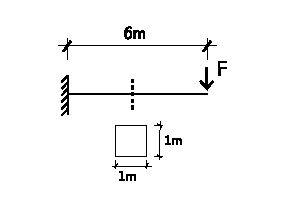
\includegraphics[width=7cm]{../Figure-files/cantilever_6.pdf}
  \caption{Problem description for cantilever beams}
  \label{fig Problem description for cantilever beam theory}
\end{figure}


The basic idea to calculate the shear deformation of a beam is 

\begin{equation}
  \delta=\frac{FL}{GA_v}
\end{equation}

where $A_v$ is the not the gross cross sectional area of the beam. $A_v$ should be the shear area. Thus,

\begin{equation}
  \kappa = \frac{A}{A_v}
\end{equation}

where $\kappa$ is the form factor, shear correction factor or shear deformation coefficient, $A$ is the gross sectional area and $A_v$ is the shear area of the section. 

The history of $\kappa$ value is long. 
\begin{enumerate}
  \item Timoshenko (1940) \footnote{Strength of materials, Timoshenko, Krieger Pub Co, 1940} define the form factor for rectangular section is 1.5. 
  \item Cowper (1970) \footnote{Cowper, G. R. "The shear coefficient in Timoshenko’s beam theory." Journal of applied mechanics 33.2 (1966): 335-340.} gave the formula for the form factor:
    \begin{equation}
      \kappa=\frac{12+11\nu}{10(1+\nu)}
    \end{equation}
  \item Renton (1991) \footnote{Renton, J. D. "Generalized beam theory applied to shear stiffness." International Journal of Solids and Structures 27.15 (1991): 1955-1967.}  provided a closed form solution for shear area of rectangular sections. For a rectangular section of depth $2a$ and breadth $2b$.
    \begin{equation}
      \kappa=\frac{6}{5}+ (\frac{\nu}{1+\nu})^2 \sum_{m=0}^{\infty}\sum_{n=1}^{\infty} \frac{144(b/a)^4}{\pi^6 (2m+1)^2 n^2 [(2m+1)^2(b/2a)^2+n^2]}
    \end{equation}
\end{enumerate}





For square cross section, $b=a$, therefore, 
\begin{equation}
  \kappa= \frac{6}{5}+ (\frac{\nu}{1+\nu})^2 \sum_{m=0}^{\infty}\sum_{n=1}^{\infty} \frac{144}{\pi^6 (2m+1)^2 n^2 [(2m+1)^2(1/2)^2+n^2]}
\end{equation}

The summation of the series are very hard. $Matlab$ and $Mathematica$ cannot solve it directly. According to the Renton (1991), the intermediate values are given by
\begin{equation}
  \kappa=\frac{6}{5}+ C_1 (\frac{\nu}{1+\nu})^2 (\frac{b}{a})^4
\end{equation}

When $b=a$, the equation becomes
\begin{equation}
  \kappa=\frac{6}{5}+ 0.1392 (\frac{\nu}{1+\nu})^2 
\end{equation}






\newpage



\section{Verification of 8NodeBrick elements}
\vskip 24pt

\subsection{Verification of 8NodeBrick cantilever beams}




Problem description: Length=6m, Width=1m, Height=1m, Force=100N, E=1E8Pa, $\nu=0.0$. Use the shear deformation coefficient $\kappa=1.2$. The force direction was shown in Figure (\ref{fig Problem description for cantilever beams}). 

\begin{figure}[H]
  \centering
  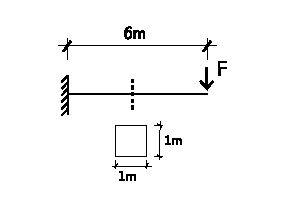
\includegraphics[width=7cm]{../Figure-files/cantilever_6.pdf}
  \caption{Problem description for cantilever beams}
  \label{fig Problem description for cantilever beams}
\end{figure}


Theoretical displacement (bending and shear deformation):
\begin{equation}
  \begin{aligned}
  d &=\frac{FL^3}{3EI}+\frac{FL}{GA_v} \\
  &= \frac{FL^3}{3E\frac{bh^3}{12}}+\frac{FL}{\frac{E}{2(1+\nu)} \frac{bh}{\kappa}} \\ 
    &= \frac{100 N \times 6^3 m^3}{3\times 10^8 N/m^2 \times \frac{1}{12} m^4}+ 
    \frac{100 N\times 6 m}{\frac{10}{2} \times 10^7 N/m^2\times 1 m^2 \times \frac{5}{6}} \\ 
    &=8.64\times 10^{-4} m + 0.144 \times 10^{-4} m   \\
   & =8.784\times 10^{-4} \ m
   \end{aligned}
\end{equation}



Numerical model:



The 8NodeBrick elements were shown in Figure (\ref{fig 8NodeBrick elements for cantilever beams}).

\begin{figure}[H]
  \centering
  \begin{subfigure}{0.5\textwidth}
    \centering
    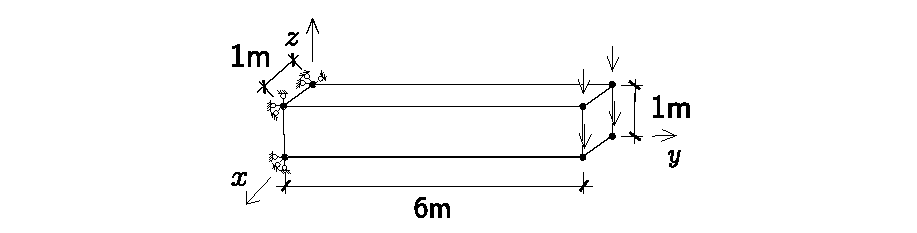
\includegraphics[width=9cm]{../Figure-files/beam_8brick_1div.pdf}
    \caption{One 8NodeBrick element}
  \end{subfigure}
  \vskip 8pt
  \begin{subfigure}{0.5\textwidth}
    \centering
    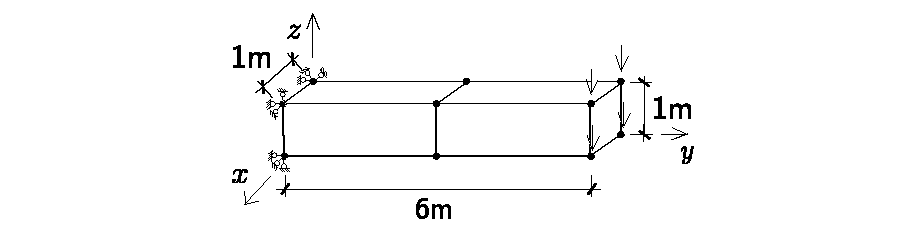
\includegraphics[width=9cm]{../Figure-files/beam_8brick_2div.pdf}
    \caption{Two 8NodeBrick elements}
  \end{subfigure}
  \vskip 8pt
  \begin{subfigure}{0.5\textwidth}
    \centering
    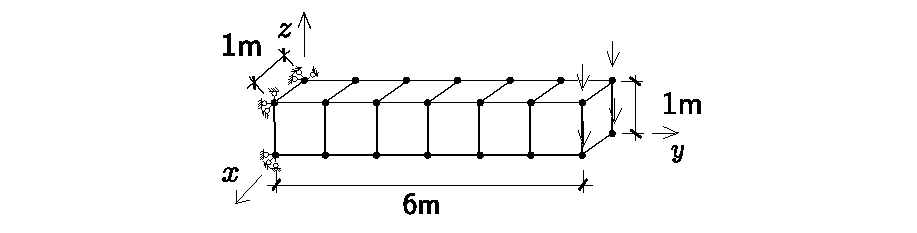
\includegraphics[width=9cm]{../Figure-files/beam_8brick_6div.pdf}
    \caption{Six 8NodeBrick elements}
  \end{subfigure}
  \captionsetup{justification=centering,margin=3cm}
  \caption{8NodeBrick elements for cantilever beams}
  \label{fig 8NodeBrick elements for cantilever beams}
\end{figure}


% \begin{figure}[H]
%   \centering
%   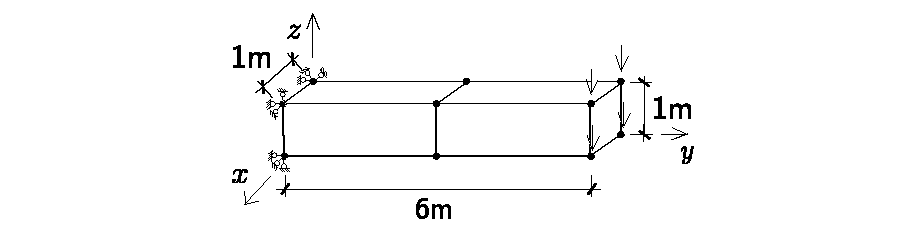
\includegraphics[width=9cm]{../Figure-files/beam_8brick_2div.pdf}
%   % \caption{}
%   % \label{}
% \end{figure}

% \begin{figure}[H]
%   \centering
%   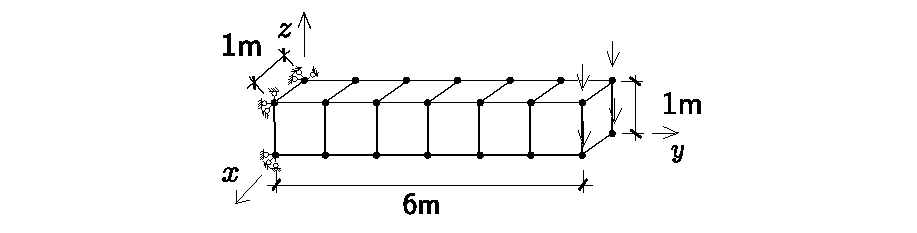
\includegraphics[width=9cm]{../Figure-files/beam_8brick_6div.pdf}
%   % \caption{}
%   % \label{}
% \end{figure}



An example ESSI script is shown below.




All the ESSI results were listed in Table (\ref{table 8NodeBrick cantilever beams results for different element number}). 
The theoretical solution is 8.784E-04 $m$.
\begin{table}[H]
  \centering
    \caption{Results for 8NodeBrick cantilever beams of different element numbers}
    \begin{tabular}{|c|c|c|c|}
      \hline
      Element number & 1        & 2        & 6         \\  \hline
      8NodeBrick     & 4.61E-05 $m$ & 1.59E-04 $m$ & 5.84E-04 $m$     \\ \hline
      Error           & 94.75\%  & 81.87\%  & 33.52\%           \\ 
      \hline 
    \end{tabular}
    \label{table 8NodeBrick cantilever beams results for different element number}
\end{table}

The errors were plotted in Figure (\ref{fig error 8NodeBrick cantilever beam for different element number}).
\begin{figure}[H]
  % \centering
  % \begin{subfigure}{0.5\textwidth}
    \centering
    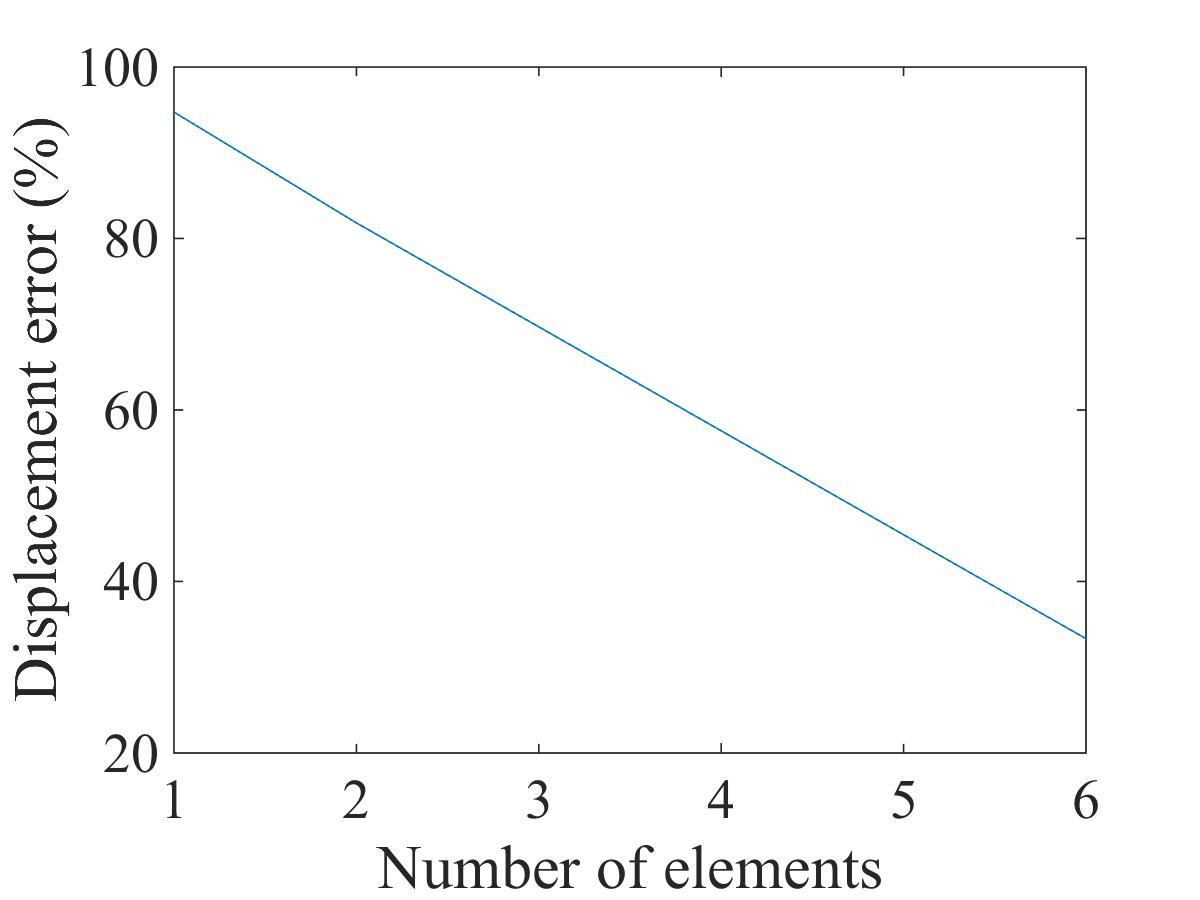
\includegraphics[width=6cm]{../Figure-files/error8brick_beam_different_element_number.jpeg}
  % \end{subfigure}
  % \begin{subfigure}{0.5\textwidth}
    % \centering
    % 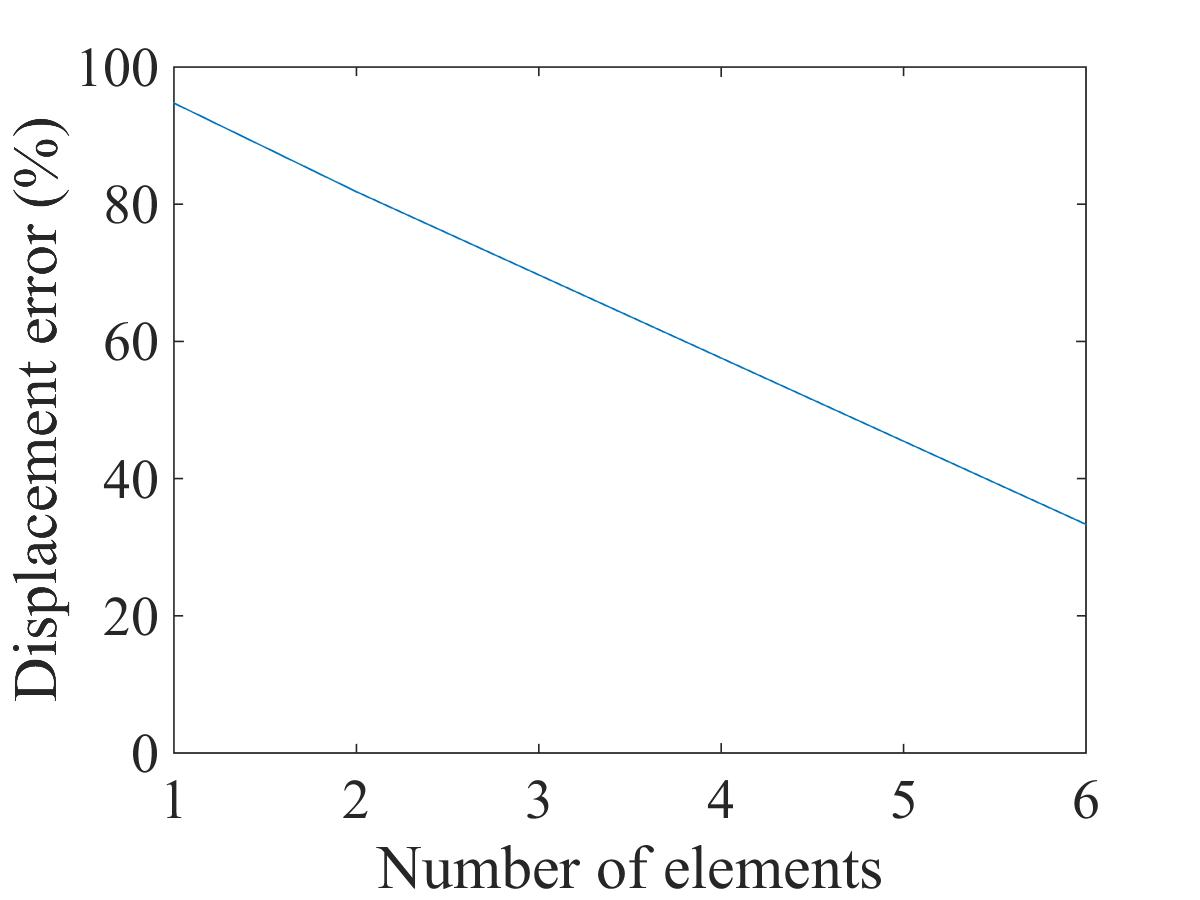
\includegraphics[width=7cm]{../Figure-files/error8brick_beam_different_element_number100.jpeg}
  % \end{subfigure}
  \captionsetup{justification=centering,margin=3cm}
  \caption{8NodeBrick cantilever beam for different element number\\
    Displacement error   versus   Number of elements}
  \label{fig error 8NodeBrick cantilever beam for different element number}
\end{figure}







The ESSI model fei files for the table above are \href{https://github.com/yuan-energy/ESSI_Verification/blob/master/8NodeBrick/cantilever_different_element_number/cantilever_different_element_number.tar.gz?raw=true}{here}






% \newpage
% \begin{itemize}
%   \item \textbf{\emph{Cantilever: different geometry}}
% \end{itemize}

% In the figures above, only the model with geometry $6m\times 1m \times 1m$ was drawed. In the ESSI models, the geometry $10m\times 1m \times 1m$ and the geometry $20m\times 1m \times 1m$ were also calculated. In three different geometry models, all the element sizes were $1m\times 1m \times 1m$. Therefore, the number of elements used in each model were $6,\ 10\ and\ 20$ respectively.

% The ESSI results for different geometry were listed in Table (\ref{table Results for 8NodeBrick cantilever beams of different geometry}). 

% \begin{table}[H]
%   \centering
%   \caption{Results for 8NodeBrick cantilever beams of different geometry}
%   \label{table Results for 8NodeBrick cantilever beams of different geometry}
%   \begin{tabular}{|c|c|c|c|c|c|}
%   \hline
%   Geometry & 8NodeBrick & Theoretical(bending) & Theoretical(shear) & Theoretical(all) & Error   \\ \hline
%   1:6      & 5.84E-04 $m$ & 8.64E-04      $m$       & 1.20E-05    $m$       & 8.76E-04  $m$       & 33.33\% \\ \hline
%   1:10     & 2.68E-03 $m$ & 4.00E-03      $m$       & 2.00E-05    $m$       & 4.02E-03  $m$       & 33.33\% \\ \hline
%   1:20     & 2.14E-02 $m$ & 3.20E-02      $m$       & 4.00E-05    $m$       & 3.20E-02  $m$       & 33.33\% \\
%   \hline
%   \end{tabular}
% \end{table}

% The ESSI model fei files for the table above are \href{https://github.com/yuan-energy/ESSI_Verification/blob/master/8NodeBrick/cantilever_different_geometry/cantilever_different_geometry.tar.gz?raw=true}{here}






\newpage
\subsection{Verification of 8NodeBrick cantilever beam for different Poisson's ratio}




Problem description: Length=6m, Width=1m, Height=1m, Force=100N, E=1E8Pa, $\nu=0.0-0.49$. The force direction was shown in Figure (\ref{fig Problem description for cantilever beams of different Poisson's ratios}). 

\begin{figure}[H]
  \centering
  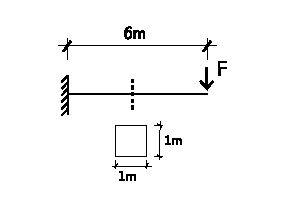
\includegraphics[width=7cm]{../Figure-files/cantilever_6.pdf}
  \caption{Problem description for cantilever beams of different Poisson's ratios}
  \label{fig Problem description for cantilever beams of different Poisson's ratios}
\end{figure}

The theoretical solution for $\nu=0.0$ was calculated below, while the solution for other Poisson's ratio were calculated by the similar process. 

Theoretical displacement (bending and shear deformation):
\begin{equation}
  \begin{aligned}
  d &=\frac{FL^3}{3EI}+\frac{FL}{GA_v} \\
  &= \frac{FL^3}{3E\frac{bh^3}{12}}+\frac{FL}{\frac{E}{2(1+\nu)} \frac{bh}{\kappa}} \\ 
    &= \frac{100 N \times 6^3 m^3}{3\times 10^8 N/m^2 \times \frac{1}{12} m^4}+ 
    \frac{100 N\times 6 m}{\frac{10}{2} \times 10^7 N/m^2\times 1 m^2 \times \frac{5}{6}} \\ 
    &=8.64\times 10^{-4} m + 0.144 \times 10^{-4} m   \\
   & =8.784\times 10^{-4} \ m
   \end{aligned}
\end{equation}

The rotation angle at the end:
\begin{equation}
  \theta =\frac{FL^2}{2EI} 
   =\frac{100 N \times 6^2 m^2} {2\times 10^8 N/m^2 \times \frac{1}{12} m^4} 
 =2.16 \times 10^{-4} \ rad = 0.0124 \degree 
\end{equation}

The 8NodeBrick elements for cantilever beams of different Poisson's ratios were shown in Figure (\ref{fig 8NodeBrick elements for cantilever beams of different Poisson's ratios}):
\begin{figure}[H]
  \centering
  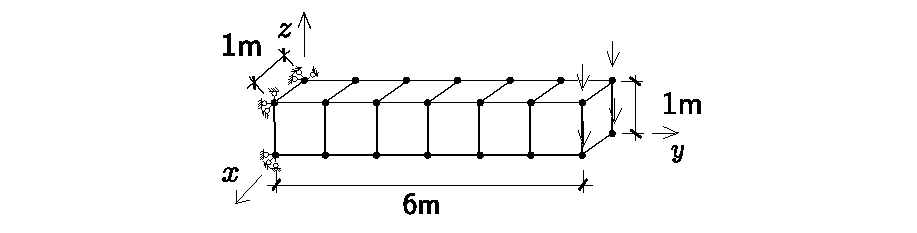
\includegraphics[width=9cm]{../Figure-files/beam_8brick_6div.pdf}
  \caption{8NodeBrick elements for cantilever beams of different Poisson's ratios}
  \label{fig 8NodeBrick elements for cantilever beams of different Poisson's ratios}
\end{figure}


All the displacement results were listed in Table (\ref{table Displacement results for 8NodeBrick cantilever beams of different Poisson ratios}) - (\ref{table Displacement results for 8NodeBrick cantilever beams of different Poisson ratios div4}). 

\begin{table}[H]
  \centering
  \captionsetup{justification=centering,margin=3cm}
  \caption{\emph{\textbf{Displacement}} results for 8NodeBrick cantilever beams with \textcolor{red}{element side length 1 m}}
  \label{table Displacement results for 8NodeBrick cantilever beams of different Poisson ratios}
  \begin{tabular}{|c|c|c|c|c|c|}
    \hline 
\tabincell{c}{Poisson's \\ ratio}    & \tabincell{c}{8NodeBrick\\displacement} & \tabincell{c}{Theory displacement\\(bending)} & \tabincell{c}{Theory displacement\\(shear)} & \tabincell{c}{Theory\\displacement(all)}   & Error \\ \hline
0.00 & 5.840E-04 $m$ & 8.640E-04 $m$ & 1.440E-05 $m$  & 8.784E-04 $m$  & 33.52\%   \\ \hline
0.05 & 5.924E-04 $m$ & 8.640E-04 $m$ & 1.512E-05 $m$  & 8.791E-04 $m$  & 32.62\%   \\ \hline
0.10 & 5.969E-04 $m$ & 8.640E-04 $m$ & 1.586E-05 $m$  & 8.799E-04 $m$  & 32.16\%   \\ \hline
0.15 & 5.971E-04 $m$ & 8.640E-04 $m$ & 1.659E-05 $m$  & 8.806E-04 $m$  & 32.20\%   \\ \hline
0.20 & 5.922E-04 $m$ & 8.640E-04 $m$ & 1.734E-05 $m$  & 8.813E-04 $m$  & 32.81\%   \\ \hline
0.25 & 5.814E-04 $m$ & 8.640E-04 $m$ & 1.808E-05 $m$  & 8.821E-04 $m$  & 34.09\%   \\ \hline
0.30 & 5.634E-04 $m$ & 8.640E-04 $m$ & 1.884E-05 $m$  & 8.828E-04 $m$  & 36.19\%   \\ \hline
0.35 & 5.364E-04 $m$ & 8.640E-04 $m$ & 1.959E-05 $m$  & 8.836E-04 $m$  & 39.29\%   \\ \hline
0.40 & 4.970E-04 $m$ & 8.640E-04 $m$ & 2.035E-05 $m$  & 8.844E-04 $m$  & 43.80\%   \\ \hline
0.45 & 4.353E-04 $m$ & 8.640E-04 $m$ & 2.111E-05 $m$  & 8.851E-04 $m$  & 50.82\%   \\ \hline
0.49 & 3.142E-04 $m$ & 8.640E-04 $m$ & 2.173E-05 $m$  & 8.857E-04 $m$  & 64.52\%   \\ \hline
  \end{tabular}
  % \caption{}
\end{table}



Then, in the same geometry, the element side length was cut into 0.5m. 

\begin{table}[H]
  \centering
  \captionsetup{justification=centering,margin=3cm}
  \caption{\emph{\textbf{Displacement}} results for 8NodeBrick cantilever beams with \textcolor{red}{element side length 0.5 m}}
  \label{table Displacement results for 8NodeBrick cantilever beams of different Poisson ratios div2}
  \begin{tabular}{|c|c|c|c|c|c|}
    \hline 
\tabincell{c}{Poisson's \\ ratio}    & \tabincell{c}{8NodeBrick\\displacement} & \tabincell{c}{Theory displacement\\(bending)} & \tabincell{c}{Theory displacement\\(shear)} & \tabincell{c}{Theory\\displacement(all)}   & Error \\ \hline
0.00 & 7.787E-04 $m$ & 8.640E-04 $m$ & 1.440E-05 $m$  & 8.784E-04 $m$ & 11.35\%    \\ \hline
0.05 & 7.824E-04 $m$ & 8.640E-04 $m$ & 1.512E-05 $m$  & 8.791E-04 $m$ & 11.00\%    \\ \hline
0.10 & 7.839E-04 $m$ & 8.640E-04 $m$ & 1.586E-05 $m$  & 8.799E-04 $m$ & 10.91\%    \\ \hline
0.15 & 7.829E-04 $m$ & 8.640E-04 $m$ & 1.659E-05 $m$  & 8.806E-04 $m$ & 11.09\%    \\ \hline
0.20 & 7.790E-04 $m$ & 8.640E-04 $m$ & 1.734E-05 $m$  & 8.813E-04 $m$ & 11.61\%    \\ \hline
0.25 & 7.717E-04 $m$ & 8.640E-04 $m$ & 1.808E-05 $m$  & 8.821E-04 $m$ & 12.51\%    \\ \hline
0.30 & 7.597E-04 $m$ & 8.640E-04 $m$ & 1.884E-05 $m$  & 8.828E-04 $m$ & 13.95\%    \\ \hline
0.35 & 7.406E-04 $m$ & 8.640E-04 $m$ & 1.959E-05 $m$  & 8.836E-04 $m$ & 16.18\%    \\ \hline
0.40 & 7.089E-04 $m$ & 8.640E-04 $m$ & 2.035E-05 $m$  & 8.844E-04 $m$ & 19.84\%    \\ \hline
0.45 & 6.466E-04 $m$ & 8.640E-04 $m$ & 2.111E-05 $m$  & 8.851E-04 $m$ & 26.95\%    \\ \hline
0.49 & 4.990E-04 $m$ & 8.640E-04 $m$ & 2.173E-05 $m$  & 8.857E-04 $m$ & 43.66\%    \\ \hline
  \end{tabular}
  % \caption{}
\end{table}

Finally, in the same geometry, the element side length was cut into 0.25m. 

\begin{table}[H]
  \centering
  \captionsetup{justification=centering,margin=3cm}
  \caption{\emph{\textbf{Displacement}} results for 8NodeBrick cantilever beams with \textcolor{red}{element side length 0.25 m}}
  \label{table Displacement results for 8NodeBrick cantilever beams of different Poisson ratios div4}
  \begin{tabular}{|c|c|c|c|c|c|}
    \hline 
\tabincell{c}{Poisson's \\ ratio}    & \tabincell{c}{8NodeBrick\\displacement} & \tabincell{c}{Theory displacement\\(bending)} & \tabincell{c}{Theory displacement\\(shear)} & \tabincell{c}{Theory\\displacement(all)}   & Error \\ \hline
0.00 & 8.511E-04 $m$ & 8.640E-04 $m$ & 1.440E-05 $m$  & 8.784E-04 $m$  & 3.11\%     \\ \hline
0.05 & 8.525E-04 $m$ & 8.640E-04 $m$ & 1.512E-05 $m$  & 8.791E-04 $m$  & 3.03\%     \\ \hline
0.10 & 8.527E-04 $m$ & 8.640E-04 $m$ & 1.586E-05 $m$  & 8.799E-04 $m$  & 3.09\%     \\ \hline
0.15 & 8.518E-04 $m$ & 8.640E-04 $m$ & 1.659E-05 $m$  & 8.806E-04 $m$  & 3.27\%     \\ \hline
0.20 & 8.494E-04 $m$ & 8.640E-04 $m$ & 1.734E-05 $m$  & 8.813E-04 $m$  & 3.62\%     \\ \hline
0.25 & 8.455E-04 $m$ & 8.640E-04 $m$ & 1.808E-05 $m$  & 8.821E-04 $m$  & 4.15\%     \\ \hline
0.30 & 8.393E-04 $m$ & 8.640E-04 $m$ & 1.884E-05 $m$  & 8.828E-04 $m$  & 4.93\%     \\ \hline
0.35 & 8.299E-04 $m$ & 8.640E-04 $m$ & 1.959E-05 $m$  & 8.836E-04 $m$  & 6.08\%     \\ \hline
0.40 & 8.141E-04 $m$ & 8.640E-04 $m$ & 2.035E-05 $m$  & 8.844E-04 $m$  & 7.94\%     \\ \hline
0.45 & 7.801E-04 $m$ & 8.640E-04 $m$ & 2.111E-05 $m$  & 8.851E-04 $m$  & 11.86\%    \\ \hline
0.49 & 6.603E-04 $m$ & 8.640E-04 $m$ & 2.173E-05 $m$  & 8.857E-04 $m$  & 25.45\%    \\ \hline
  \end{tabular}
  % \caption{}
\end{table}





% \begin{table}[H]
%   \centering
%   \caption{\emph{\textbf{Displacement}} results for 8NodeBrick cantilever beams of different Poisson's ratios}
%   \label{table Displacement results for 8NodeBrick cantilever beams of different Poisson ratios}
%   \begin{tabular}{|c|c|c|c|c|c|}
%     \hline 
% \tabincell{c}{Poisson's \\ ratio}    & \tabincell{c}{8NodeBrick\\displacement} & \tabincell{c}{Theory displacement\\(bending)} & \tabincell{c}{Theory displacement\\(shear)} & \tabincell{c}{Theory\\displacement(all)}   & Error \\ \hline
% 0.00 & 5.840E-04 $m$ & 8.640E-04 $m$ & 1.200E-05  $m$  & 8.740E-04 $m$  & 33.33\%    \\ \hline
% 0.05 & 5.924E-04 $m$ & 8.640E-04 $m$ & 1.260E-05  $m$  & 8.745E-04 $m$  & 32.42\%    \\ \hline
% 0.10 & 5.969E-04 $m$ & 8.640E-04 $m$ & 1.320E-05  $m$  & 8.750E-04 $m$  & 31.95\%    \\ \hline
% 0.15 & 5.971E-04 $m$ & 8.640E-04 $m$ & 1.380E-05  $m$  & 8.755E-04 $m$  & 31.98\%    \\ \hline
% 0.20 & 5.922E-04 $m$ & 8.640E-04 $m$ & 1.440E-05  $m$  & 8.760E-04 $m$  & 32.58\%    \\ \hline
% 0.25 & 5.814E-04 $m$ & 8.640E-04 $m$ & 1.500E-05  $m$  & 8.765E-04 $m$  & 33.86\%    \\ \hline
% 0.30 & 5.634E-04 $m$ & 8.640E-04 $m$ & 1.560E-05  $m$  & 8.770E-04 $m$  & 35.95\%    \\ \hline
% 0.35 & 5.364E-04 $m$ & 8.640E-04 $m$ & 1.620E-05  $m$  & 8.775E-04 $m$  & 39.06\%    \\ \hline
% 0.40 & 4.970E-04 $m$ & 8.640E-04 $m$ & 1.680E-05  $m$  & 8.780E-04 $m$  & 43.57\%    \\ \hline
% 0.45 & 4.353E-04 $m$ & 8.640E-04 $m$ & 1.740E-05  $m$  & 8.785E-04 $m$  & 50.61\%    \\ \hline
% 0.49 & 3.142E-04 $m$ & 8.640E-04 $m$ & 1.788E-05  $m$  & 8.789E-04 $m$  & 64.37\%    \\ \hline
%   \end{tabular}
%   % \caption{}
% \end{table}



The errors were plotted in Figure (\ref{fig error 8NodeBrick cantilever beam for different Poisson's ratio}).
\begin{figure}[H]
  % \centering
  \begin{subfigure}{0.5\textwidth}
    \centering
    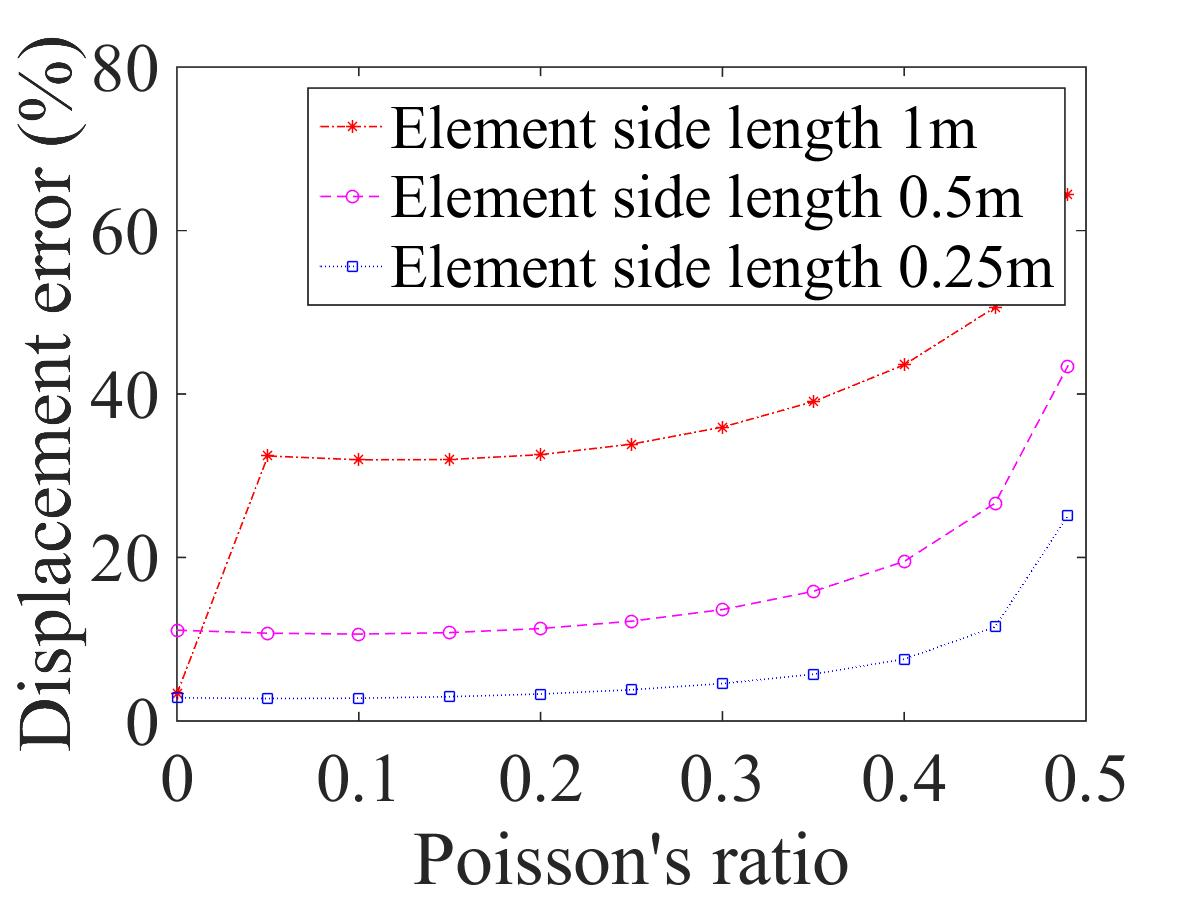
\includegraphics[width=6cm]{../Figure-files/error8brick_beam_different_poisson_ratio_disp_div.jpeg}
    \caption{Error scale 0\% - 80\%}
  \end{subfigure}
  \begin{subfigure}{0.5\textwidth}
    \centering
    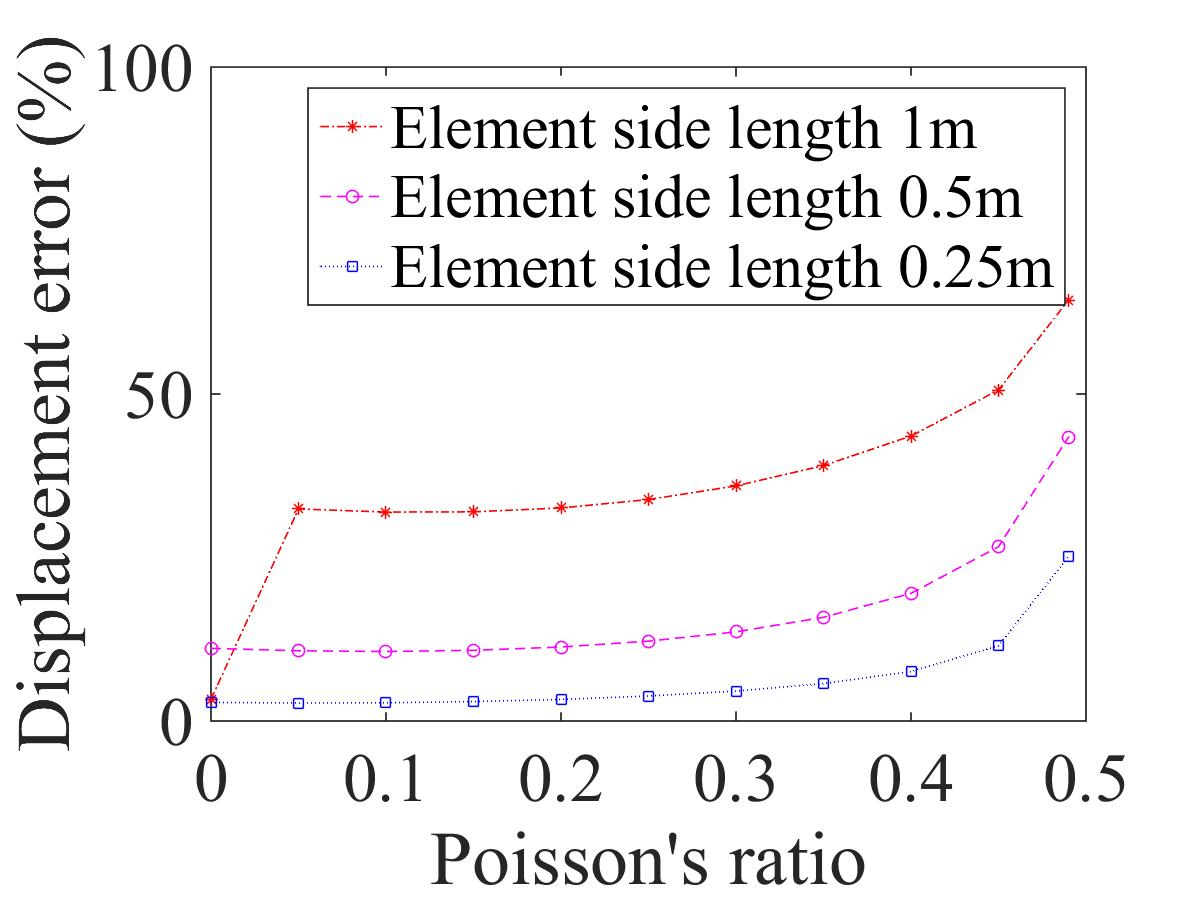
\includegraphics[width=6cm]{../Figure-files/error8brick_beam_different_poisson_ratio_disp_div100.jpeg}
    \caption{Error scale 0\% - 100\%}
  \end{subfigure}
  \captionsetup{justification=centering,margin=3cm}
  \caption{8NodeBrick cantilever beam for different Poisson's ratio\\
      \emph{\textbf{Displacement error}}   versus   Poisson's ratio}
  \label{fig error 8NodeBrick cantilever beam for different Poisson's ratio}
\end{figure}


The angle results were listed in Table (\ref{table angle results for 8NodeBrick cantilever beams of different Poissons ratios}).
\begin{table}[H]
  \centering
  \captionsetup{justification=centering,margin=3cm}
  \caption{\emph{\textbf{Rotation angle}} results for 8NodeBrick cantilever beams with \textcolor{red}{element side length 1 m}}
  \label{table angle results for 8NodeBrick cantilever beams of different Poissons ratios}
\begin{tabular}{|c|c|c|c|}
\hline
\tabincell{c}{Poisson's \\ ratio} & \tabincell{c}{8NodeBrick \\ angle (unit:\degree)}  & \tabincell{c}{Theory angle\\(unit:\degree)}  & Error   \\ \hline
0.00            & 8.25E-03   & 1.24E-02     & 33.46\% \\ \hline
0.05            & 8.36E-03   & 1.24E-02     & 32.55\% \\ \hline
0.10            & 8.42E-03   & 1.24E-02     & 32.08\% \\ \hline
0.15            & 8.42E-03   & 1.24E-02     & 32.10\% \\ \hline
0.20            & 8.35E-03   & 1.24E-02     & 32.67\% \\ \hline
0.25            & 8.20E-03   & 1.24E-02     & 33.90\% \\ \hline
0.30            & 7.95E-03   & 1.24E-02     & 35.89\% \\ \hline
0.35            & 7.59E-03   & 1.24E-02     & 38.83\% \\ \hline
0.40            & 7.07E-03   & 1.24E-02     & 43.00\% \\ \hline
0.45            & 6.30E-03   & 1.24E-02     & 49.21\% \\ \hline
0.49            & 4.93E-03   & 1.24E-02     & 60.20\% \\
\hline
\end{tabular}
  % \caption{}
\end{table}



Then, in the same geometry, element side length was cut into 0.5m. The angle results were listed in Table (\ref{table angle results for 8NodeBrick cantilever beams of different Poissons ratios div2}).
\begin{table}[H]
  \centering
  \captionsetup{justification=centering,margin=3cm}
  \caption{\emph{\textbf{Rotation angle}} results for 8NodeBrick cantilever beams with with \textcolor{red}{element side length 0.5 m}}
  \label{table angle results for 8NodeBrick cantilever beams of different Poissons ratios div2}
\begin{tabular}{|c|c|c|c|}
\hline
\tabincell{c}{Poisson's \\ ratio} & \tabincell{c}{8NodeBrick \\ angle (unit:\degree)}  & \tabincell{c}{Theory angle\\(unit:\degree)}  & Error   \\ \hline
0.00            & 1.10E-02 & 1.24E-02 & 11.28\% \\ \hline
0.05            & 1.10E-02 & 1.24E-02 & 10.91\% \\ \hline
0.10            & 1.11E-02 & 1.24E-02 & 10.78\% \\ \hline
0.15            & 1.10E-02 & 1.24E-02 & 10.90\% \\ \hline
0.20            & 1.10E-02 & 1.24E-02 & 11.32\% \\ \hline
0.25            & 1.09E-02 & 1.24E-02 & 12.09\% \\ \hline
0.30            & 1.07E-02 & 1.24E-02 & 13.33\% \\ \hline
0.35            & 1.05E-02 & 1.24E-02 & 15.29\% \\ \hline
0.40            & 1.01E-02 & 1.24E-02 & 18.53\% \\ \hline
0.45            & 9.32E-03 & 1.24E-02 & 24.87\% \\ \hline
0.49            & 7.52E-03 & 1.24E-02 & 39.35\% \\
\hline
\end{tabular}
  % \caption{}
\end{table}





Finally, in the same geometry, element side length was cut into 0.25m. The angle results were listed in Table (\ref{table angle results for 8NodeBrick cantilever beams of different Poissons ratios div4}).
\begin{table}[H]
  \centering
  \captionsetup{justification=centering,margin=3cm}
  \caption{\emph{\textbf{Rotation angle}} results for 8NodeBrick cantilever beams with with \textcolor{red}{element side length 0.25 m}}
  \label{table angle results for 8NodeBrick cantilever beams of different Poissons ratios div4}
\begin{tabular}{|c|c|c|c|}
\hline
\tabincell{c}{Poisson's \\ ratio} & \tabincell{c}{8NodeBrick \\ angle (unit:\degree)}  & \tabincell{c}{Theory angle\\(unit:\degree)}  & Error   \\ \hline
0.00            & 1.20E-02 & 1.24E-02 & 3.06\%  \\ \hline
0.05            & 1.20E-02 & 1.24E-02 & 2.97\%  \\ \hline
0.10            & 1.20E-02 & 1.24E-02 & 2.99\%  \\ \hline
0.15            & 1.20E-02 & 1.24E-02 & 3.12\%  \\ \hline
0.20            & 1.20E-02 & 1.24E-02 & 3.38\%  \\ \hline
0.25            & 1.19E-02 & 1.24E-02 & 3.79\%  \\ \hline
0.30            & 1.19E-02 & 1.24E-02 & 4.40\%  \\ \hline
0.35            & 1.17E-02 & 1.24E-02 & 5.33\%  \\ \hline
0.40            & 1.15E-02 & 1.24E-02 & 6.87\%  \\ \hline
0.45            & 1.11E-02 & 1.24E-02 & 10.22\% \\ \hline
0.49            & 9.64E-03 & 1.24E-02 & 22.23\% \\
\hline
\end{tabular}
  % \caption{}
\end{table}












The errors were plotted in Figure (\ref{table angle error 8NodeBrick cantilever beam for different Poisson ratio}).

\begin{figure}[H]
  % \centering
  \begin{subfigure}{0.5\textwidth}
    \centering
    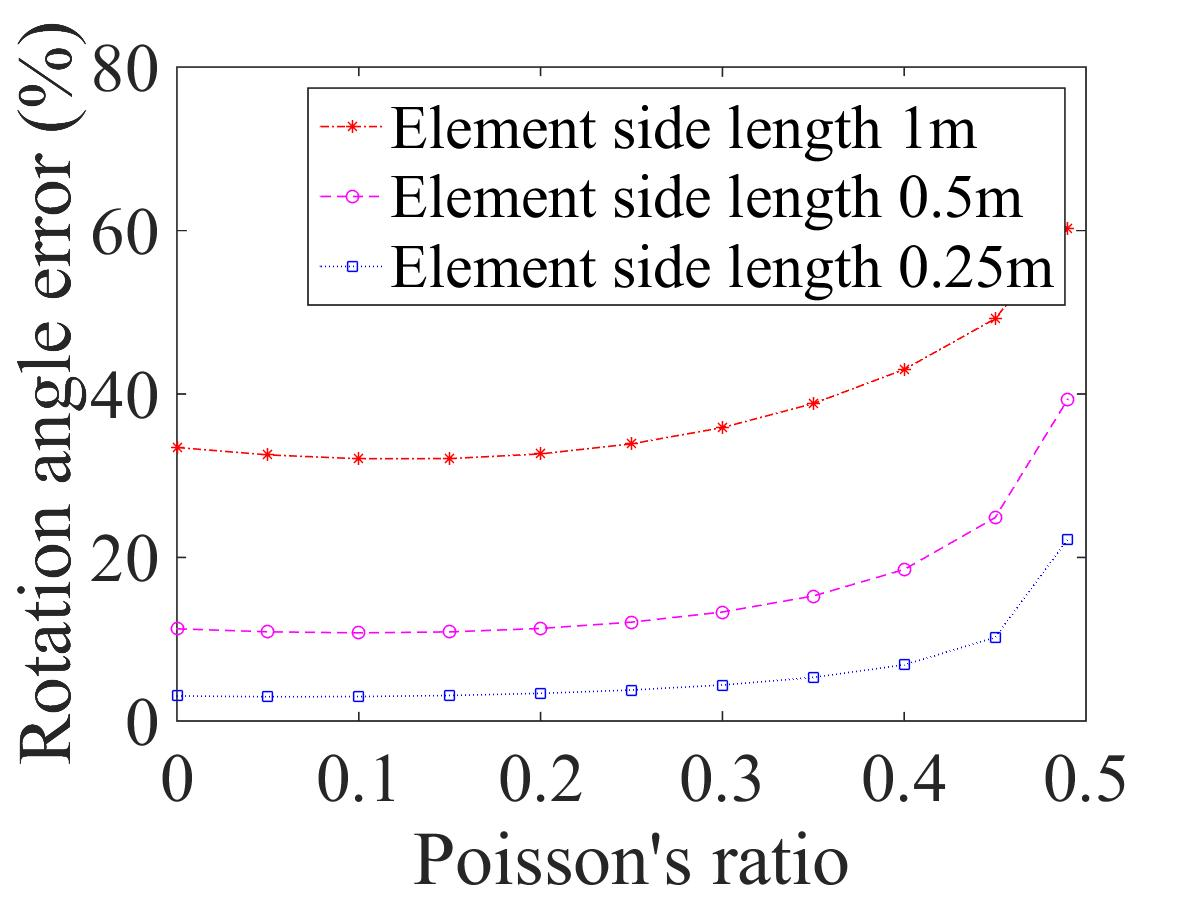
\includegraphics[width=6cm]{../Figure-files/error8brick_beam_different_poisson_ratio_angle_div.jpeg}
    \caption{Error scale 30\% - 70\%}
  \end{subfigure}
  \begin{subfigure}{0.5\textwidth}
    \centering
    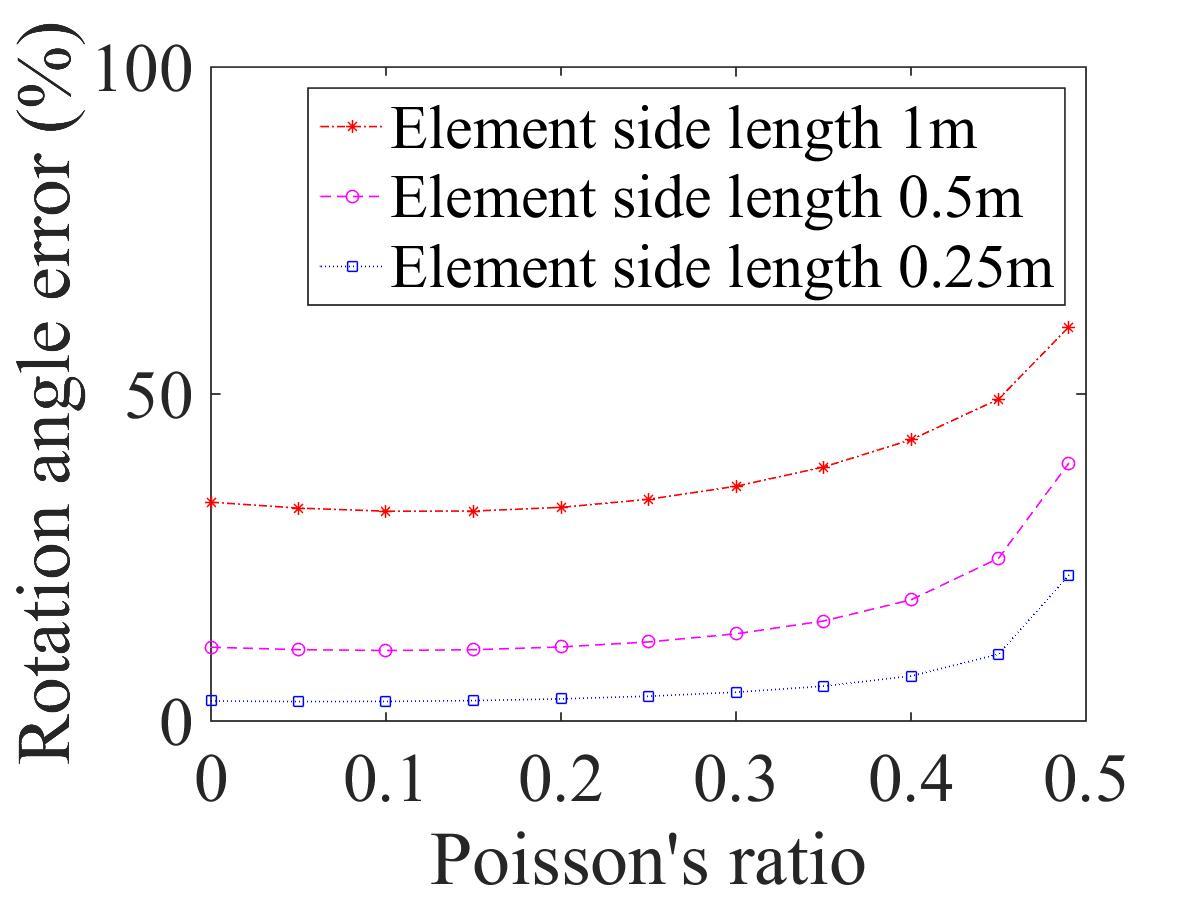
\includegraphics[width=6cm]{../Figure-files/error8brick_beam_different_poisson_ratio_angle_div100.jpeg}
    \caption{Error scale 0\% - 100\%}
  \end{subfigure}
  \captionsetup{justification=centering,margin=3cm}
  \caption{8NodeBrick cantilever beam for different Poisson's ratio\\
      \emph{\textbf{Rotation angle error}}   versus   Poisson's ratio}
  \label{table angle error 8NodeBrick cantilever beam for different Poisson ratio}
\end{figure}



The ESSI model fei files for the table above are \href{https://github.com/yuan-energy/ESSI_Verification/blob/master/8NodeBrick/cantilever_different_Poisson/cantilever_different_Poisson.tar.gz?raw=true}{here}




\newpage
\subsection{Test of irregular shaped 8NodeBrick cantilever beams}

Cantilever model was used as an example. 
Three different shapes were tested. 


In the first test, the upper two nodes of each element were moved one half element size along the $y-axis$, while the lower two nodes were kept at the same location. The element shape was shown in Figure (\ref{fig irregular shape 1 8NodeBrick cantilever beams }).

\begin{figure}[H]
  \centering
  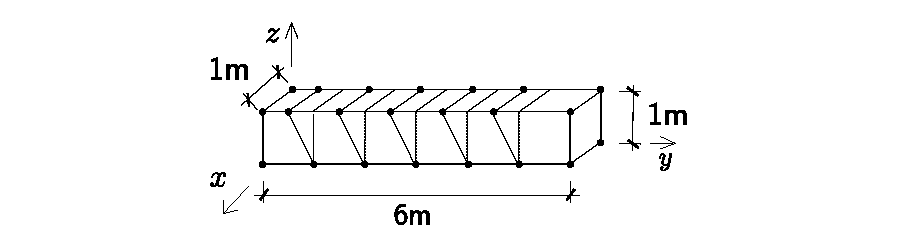
\includegraphics[width=9cm]{../Figure-files/beam_brick_shape1.pdf}
  \caption{8NodeBrick cantilever beams for irregular \textbf{\emph{Shape 1}} }
  \label{fig irregular shape 1 8NodeBrick cantilever beams }
\end{figure}


In the second test, the upper two nodes of each element were moved 90\% element size along the $y-axis$, while the lower two nodes were moved 90\% element size in the other direction along the $y-axis$. The element shape was shown in Figure (\ref{fig irregular shape 2 8NodeBrick cantilever beams }).

\begin{figure}[H]
  \centering
  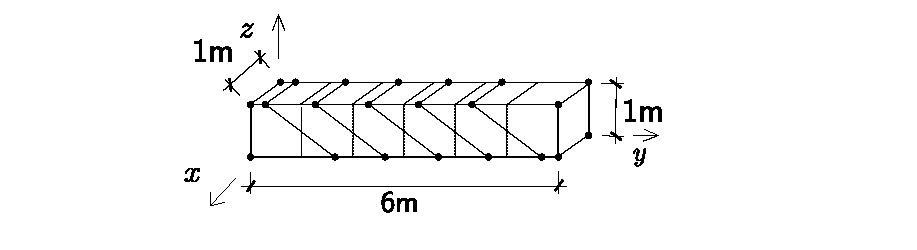
\includegraphics[width=9cm]{../Figure-files/beam_brick_shape2.pdf}
  \caption{8NodeBrick cantilever beams for irregular \textbf{\emph{Shape 2}} }
  \label{fig irregular shape 2 8NodeBrick cantilever beams }
\end{figure}



In the third test, the upper two nodes of each element were moved one half element size with different directions along the $y-axis$, while the lower two nodes were kept at the same location. The element shape was shown in Figure (\ref{fig irregular shape 3 8NodeBrick cantilever beams }).

\begin{figure}[H]
  \centering
  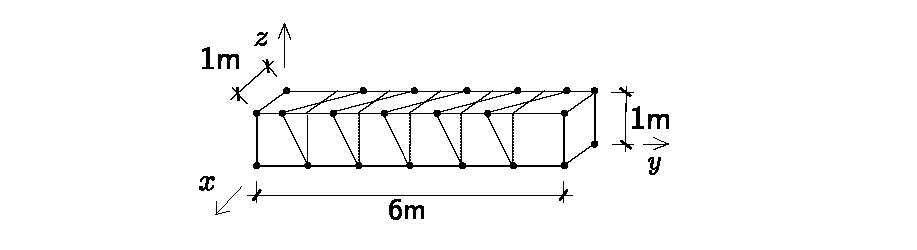
\includegraphics[width=9cm]{../Figure-files/beam_brick_shape3.pdf}
  \caption{8NodeBrick cantilever beams for irregular \textbf{\emph{Shape 3}} }
  \label{fig irregular shape 3 8NodeBrick cantilever beams }
\end{figure}

The boundary conditions were shown in Figure (\ref{fig 8NodeBrick cantilever beam boundary conditions shape 1}), (\ref{fig 8NodeBrick cantilever beam boundary conditions shape 2}) and (\ref{fig 8NodeBrick cantilever beam boundary conditions shape 3}) .

\begin{figure}[H]
  \centering
    \begin{subfigure}{0.5\textwidth}
      \centering
      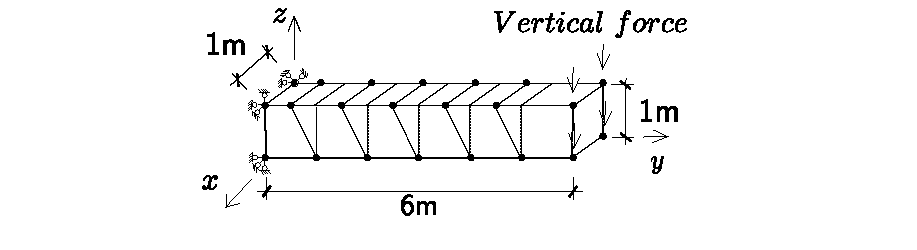
\includegraphics[width=9cm]{../Figure-files/beam_brick_shape1_vertical.pdf}
      \caption{Veritical force}
    \end{subfigure}
    \begin{subfigure}{0.5\textwidth}
      \centering
      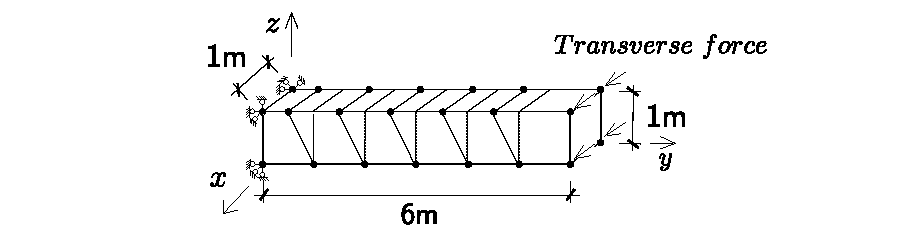
\includegraphics[width=9cm]{../Figure-files/beam_brick_shape1_horizontal.pdf}
      \caption{Horizontal force}
    \end{subfigure}
  \caption{8NodeBrick cantilever beam boundary conditions for irregular \textbf{\emph{Shape 1}} }
  \label{fig 8NodeBrick cantilever beam boundary conditions shape 1}
\end{figure}


\begin{figure}[H]
  \centering
    \begin{subfigure}{0.5\textwidth}
      \centering
      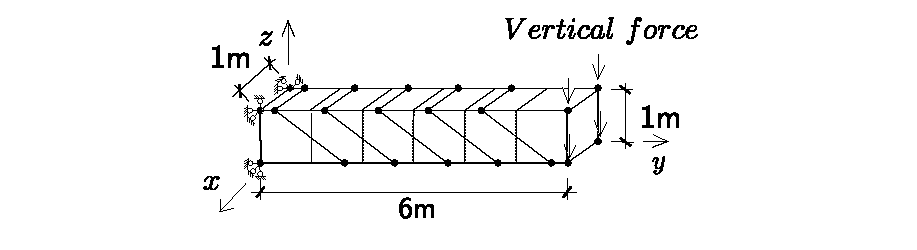
\includegraphics[width=9cm]{../Figure-files/beam_brick_shape2_vertical.pdf}
      \caption{Veritical force}
    \end{subfigure}
    \begin{subfigure}{0.5\textwidth}
      \centering
      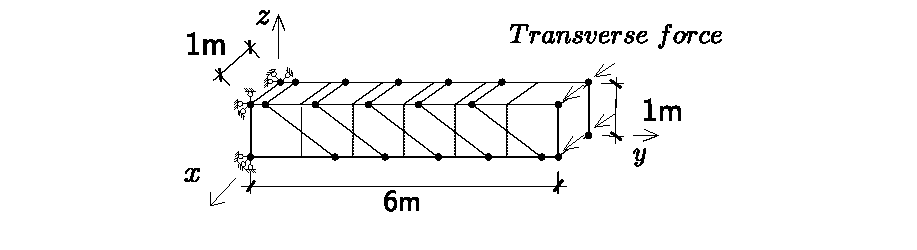
\includegraphics[width=9cm]{../Figure-files/beam_brick_shape2_horizontal.pdf}
      \caption{Horizontal force}
    \end{subfigure}
  \caption{8NodeBrick cantilever beam boundary conditions for irregular \textbf{\emph{Shape 2}} }
  \label{fig 8NodeBrick cantilever beam boundary conditions shape 2}
\end{figure}


\begin{figure}[H]
  \centering
    \begin{subfigure}{0.5\textwidth}
      \centering
      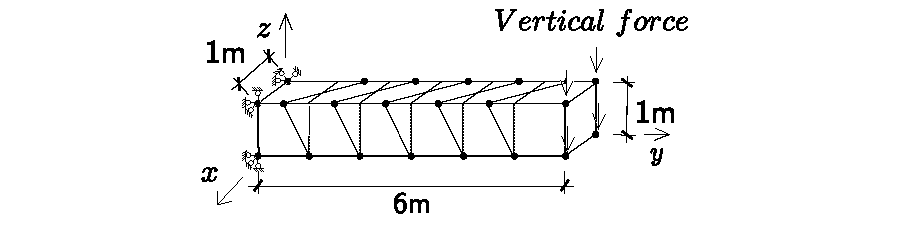
\includegraphics[width=9cm]{../Figure-files/beam_brick_shape3_vertical.pdf}
      \caption{Veritical force}
    \end{subfigure}
    \begin{subfigure}{0.5\textwidth}
      \centering
      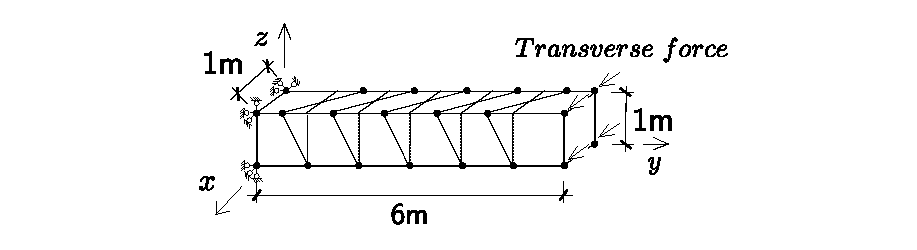
\includegraphics[width=9cm]{../Figure-files/beam_brick_shape3_horizontal.pdf}
      \caption{Horizontal force}
    \end{subfigure}
  \caption{8NodeBrick cantilever beam boundary conditions for irregular \textbf{\emph{Shape 3}} }
  \label{fig 8NodeBrick cantilever beam boundary conditions shape 3}
\end{figure}


The ESSI results were listed in Table (\ref{table Results for 8NodeBrick cantilever beams of irregular shapes}). 
\begin{table}[H]
  \centering
  \caption{Results for 8NodeBrick cantilever beams of irregular shapes}
  \label{table Results for 8NodeBrick cantilever beams of irregular shapes}
  \begin{tabular}{|c|c|c|c|c|c|}
    \hline 
    Element Type   & Force direction & Normal shape & Shape 1 & Shape 2 & Shape 3  \\ \hline 
    8NodeBrick     & Vertical ($z$)     & 5.840E-04 $m$  & 5.751E-04 $m$ & 2.959E-04 $m$ & 3.883E-04 $m$   \\ \hline
    8NodeBrick     & Transverse ($y$)      & 5.840E-04 $m$  & 4.529E-04 $m$ & 1.390E-04 $m$ & 4.744E-04 $m$   \\ \hline
    Theoretical    &      -              & 8.784E-04 $m$  & 8.784E-04 $m$ & 8.784E-04 $m$ & 8.784E-04 $m$ \\ \hline
  \end{tabular}
\end{table}

The errors were listed in Table (\ref{table Errors for irregular shaped 8NodeBrick compared to theoretical solution}) and (\ref{talbe Errors for irregular shaped 8NodeBrick compared to normal shape}).


\begin{table}[H]
  \centering
  \caption{Errors for irregular shaped 8NodeBrick compared to theoretical solution}
  \label{table Errors for irregular shaped 8NodeBrick compared to theoretical solution}
  \begin{tabular}{|c|c|c|c|c|c|}
    \hline 
    Element Type   & Force direction & Normal shape & Shape 1 & Shape 2 & Shape 3  \\ \hline 
    8NodeBrick     & Vertical ($z$)     & 33.52\% & 34.53\% & 66.31\% & 55.79\%  \\ \hline
    8NodeBrick     & Transverse ($y$)   & 33.52\% & 48.44\% & 84.18\% & 45.99\%  \\ \hline
  \end{tabular}
  % \caption{}
\end{table}

\begin{table}[H]
  \centering
  \caption{Errors for irregular shaped 8NodeBrick compared to normal shape}
  \label{talbe Errors for irregular shaped 8NodeBrick compared to normal shape}
  \begin{tabular}{|c|c|c|c|c|c|}
    \hline 
    Element Type   & Force direction & Normal shape & Shape 1 & Shape 2 & Shape 3  \\ \hline 
    8NodeBrick     & Vertical ($z$)     & 0.00\% & 1.52\%  & 49.33\% & 33.51\%       \\ \hline
    8NodeBrick     & Transverse ($y$)   & 0.00\% & 22.45\% & 76.20\% & 18.77\%       \\ \hline
  \end{tabular}
  % \caption{}
\end{table}

The ESSI model fei files for the table above are \href{https://github.com/yuan-energy/ESSI_Verification/blob/master/8NodeBrick/cantilever_irregular_element/cantilever_irregular_element.tar.gz?raw=true}{here}



% The errors were listed below, compared to the theoretical solution.
% \begin{table}[H]
%   \centering
%   \begin{tabular}{|c|c|c|c|c|}
%     \hline 
%     \multicolumn{5}{|c|}{Test for brick shape displacement errors}   \\ \hline
%     Element Type  & Normal shape & Shape 1 & Shape 2 & Shape 3  \\ \hline 
%     8NodeBrick     &     &    &   & \\ \hline
%     27NodeBrick    &     &    &   &  \\ \hline
%   \end{tabular}
%   % \caption{}
% \end{table}

\newpage
Then, the irregular beam was divided into small elements. 


Problem description: Length=12m, Width=2m, Height=2m, q=400N/m, E=1E8Pa, $\nu=0.0$. Use the shear deformation coefficient $\kappa=1.2$. The force direction was shown in Figure (\ref{fig Problem description for cantilever beams under uniform pressure}). 

\begin{figure}[H]
  \centering
  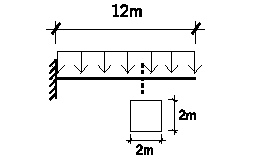
\includegraphics[width=7cm]{../Figure-files/cantilever_12_uniform_load.pdf}
  \caption{Problem description for cantilever beams under uniform load  }
  \label{fig Problem description for cantilever beams under uniform pressure}
\end{figure}


Theoretical displacement (bending and shear deformation):
\begin{equation}
  \begin{aligned}
  d &=\frac{qL^4}{8EI} + \frac{q \frac{L^2}{2}}{GA_v} \\ 
    &=\frac{qL^4}{8E\frac{bh^3}{12} }+\frac{q \frac{L^2}{2}}{\frac{E}{2(1+\nu)}\frac{bh}{\kappa}} \\
    &= \frac{400 N/m \times 12^4 m^4}{8\times 10^8 N/m^2 \times \frac{2^4}{12} m^4} 
       + \frac{400 N/m \times \frac{12^2}{2} m^2} {\frac{10^8}{2} N/m^2 \times 2m\times 2m\times \frac{5}{6}} \\ 
    &=7.776\times 10^{-3} m  +1.728\times 10^{-4} m \\
    &=7.9488\times 10^{-3} m
   \end{aligned}
\end{equation}







The ESSI displacement results were listed in Table (\ref{table Results for 8NodeBrick cantilever beams of irregular shapes with more elements}).
\begin{table}[H]
  \centering
  \caption{Results for 8NodeBrick cantilever beams of irregular shapes with more elements}
  \label{table Results for 8NodeBrick cantilever beams of irregular shapes with more elements}
\begin{tabular}{|c|c|c|c|c|c|}
\hline
\multirow{2}{*}{Element Type} & \multirow{2}{*}{Shape}  & \multirow{2}{*}{Force direction}  & \multicolumn{3}{|c|}{Number of division} \\  \cline{4-6}
                        &        &                  &  1 &  2 &  4  \\ \hline
8NodeBrick              & shape1 & Vertical ($z$)   & 5.37E-03 $m$  & 7.08E-03 $m$  & 7.71E-03  $m$ \\ \hline
8NodeBrick              & shape1 & Transverse ($y$) & 4.60E-03 $m$  & 6.66E-03 $m$  & 7.58E-03  $m$ \\ \hline
8NodeBrick              & shape2 & Vertical ($z$)   & 2.74E-03 $m$& 4.75E-03 $m$& 6.43E-03  $m$ \\ \hline
8NodeBrick              & shape2 & Transverse ($y$) & 1.46E-03 $m$& 2.72E-03 $m$& 4.63E-03  $m$ \\ \hline
8NodeBrick              & shape3 & Vertical ($z$)   & 9.21E-04 $m$  & 6.60E-03 $m$  & 7.56E-03  $m$ \\ \hline
8NodeBrick              & shape3 & Transverse ($y$) & 1.09E-03 $m$  & 6.09E-03 $m$  & 7.37E-03  $m$ \\ \hline
 \multicolumn{3}{|c|}{Theoretical solution}      & 7.95E-03 $m$  & 7.95E-03 $m$  & 7.95E-03  $m$ \\
\hline
\end{tabular}
\end{table}

The error were listed in Table (\ref{table Errors for 8NodeBrick cantilever beams of irregular shapes with more elements}). 

\begin{table}[H]
  \centering
  \caption{Errors for 8NodeBrick cantilever beams of irregular shapes with more elements}
  \label{table Errors for 8NodeBrick cantilever beams of irregular shapes with more elements}
\begin{tabular}{|c|c|c|c|c|c|}
\hline
\multirow{2}{*}{Element Type} & \multirow{2}{*}{Shape}  & \multirow{2}{*}{Force direction}  & \multicolumn{3}{|c|}{Number of division} \\  \cline{4-6}
                        &        &                  &  1 &  2 &  4  \\ \hline
8NodeBrick   & shape1      & Vertical ($z$)   & 32.42\% & 10.95\% & 3.01\%     \\ \hline
8NodeBrick   & shape1      & Transverse ($y$) & 42.16\% & 16.17\% & 4.69\%     \\ \hline
8NodeBrick   & shape2      & Vertical ($z$)   & 65.59\% & 40.22\% & 19.05\%    \\ \hline
8NodeBrick   & shape2      & Transverse ($y$) & 81.57\% & 65.76\% & 41.81\%    \\ \hline
8NodeBrick   & shape3      & Vertical ($z$)   & 88.42\% & 16.97\% & 4.89\%     \\ \hline
8NodeBrick   & shape3      & Transverse ($y$) & 86.24\% & 23.36\% & 7.28\%     \\
\hline
\end{tabular}
\end{table}



% \begin{figure}[H]
%   % \centering
%   \begin{subfigure}{0.5\textwidth}
%     \centering
%     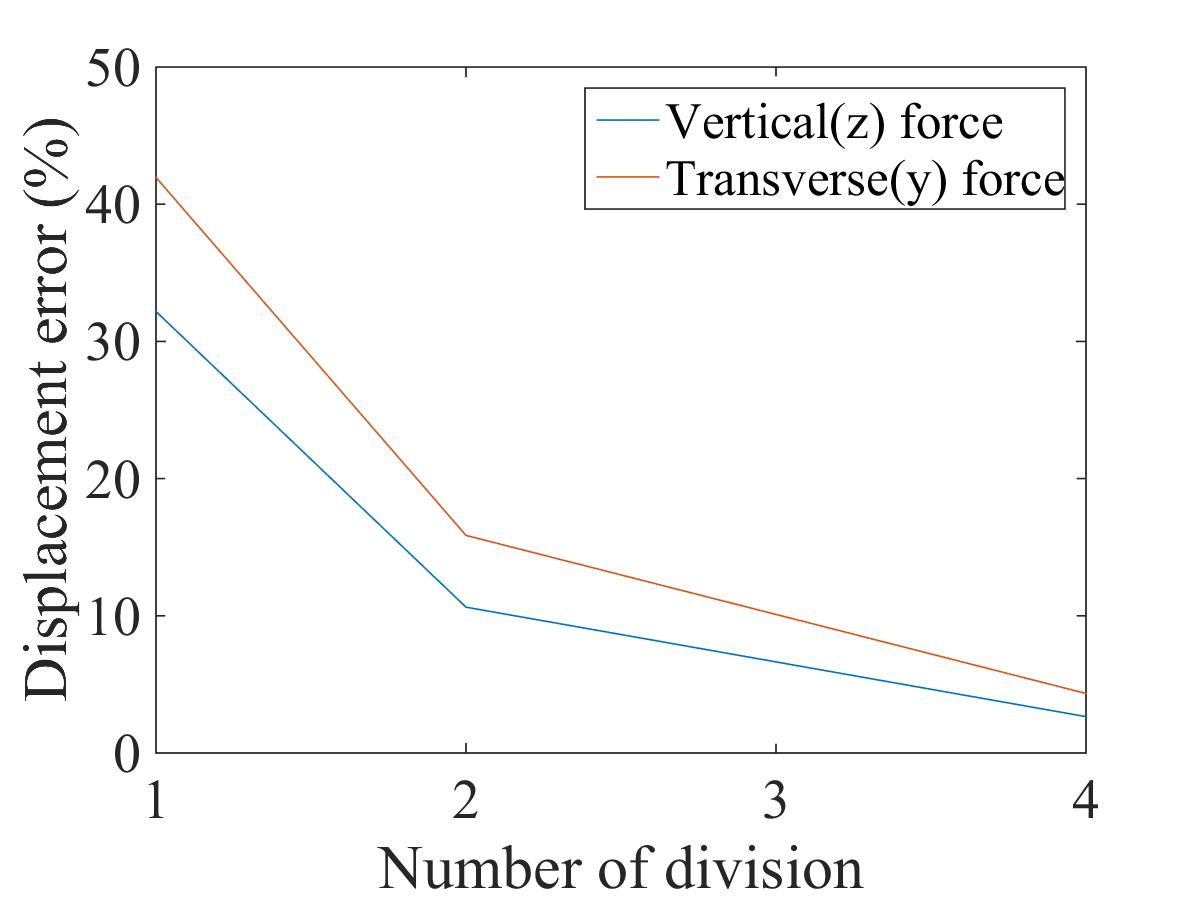
\includegraphics[width=6cm]{../Figure-files/error8brick_beam_irregular_shape1.jpeg}
%     \caption{Error scale 0\% - 50\%}
%   \end{subfigure}
%   \begin{subfigure}{0.5\textwidth}
%     \centering
%     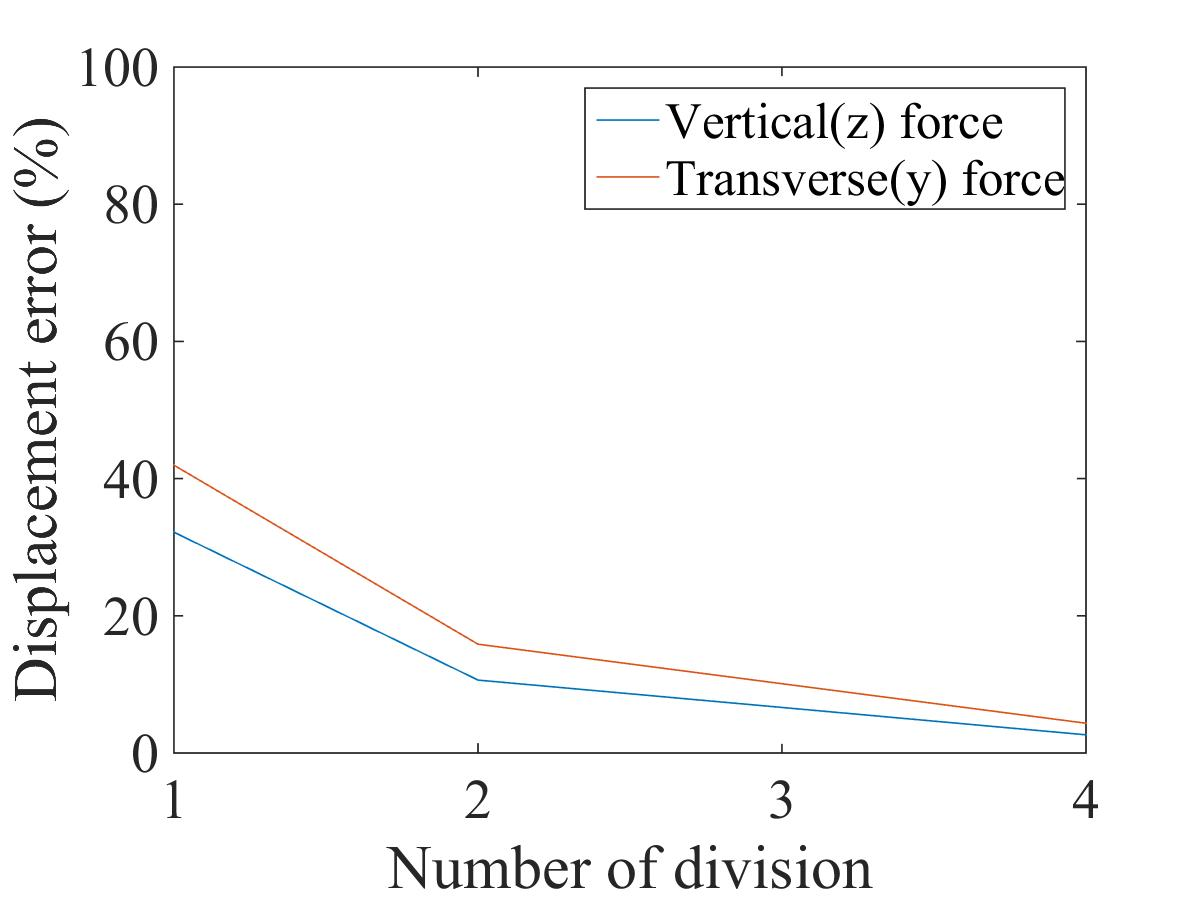
\includegraphics[width=6cm]{../Figure-files/error8brick_beam_irregular_shape1100.jpeg}
%     \caption{Error scale 0\% - 100\%}
%   \end{subfigure}
%   \captionsetup{justification=centering,margin=3cm}
%   \caption{8NodeBrick cantilever beam for irregular Shape 1\\
%       Displacement error   versus   Number of division}
%   % \caption{}
%   % \label{}
% \end{figure}

The errors were shown in Figure (\ref{fig shape 1 8NodeBrick cantilever beam for irregular more elements}), (\ref{fig shape 2 8NodeBrick cantilever beam for irregular more elements}) and (\ref{fig shape 3 8NodeBrick cantilever beam for irregular more elements}). 
\begin{figure}[H]
  % \centering
    \centering
    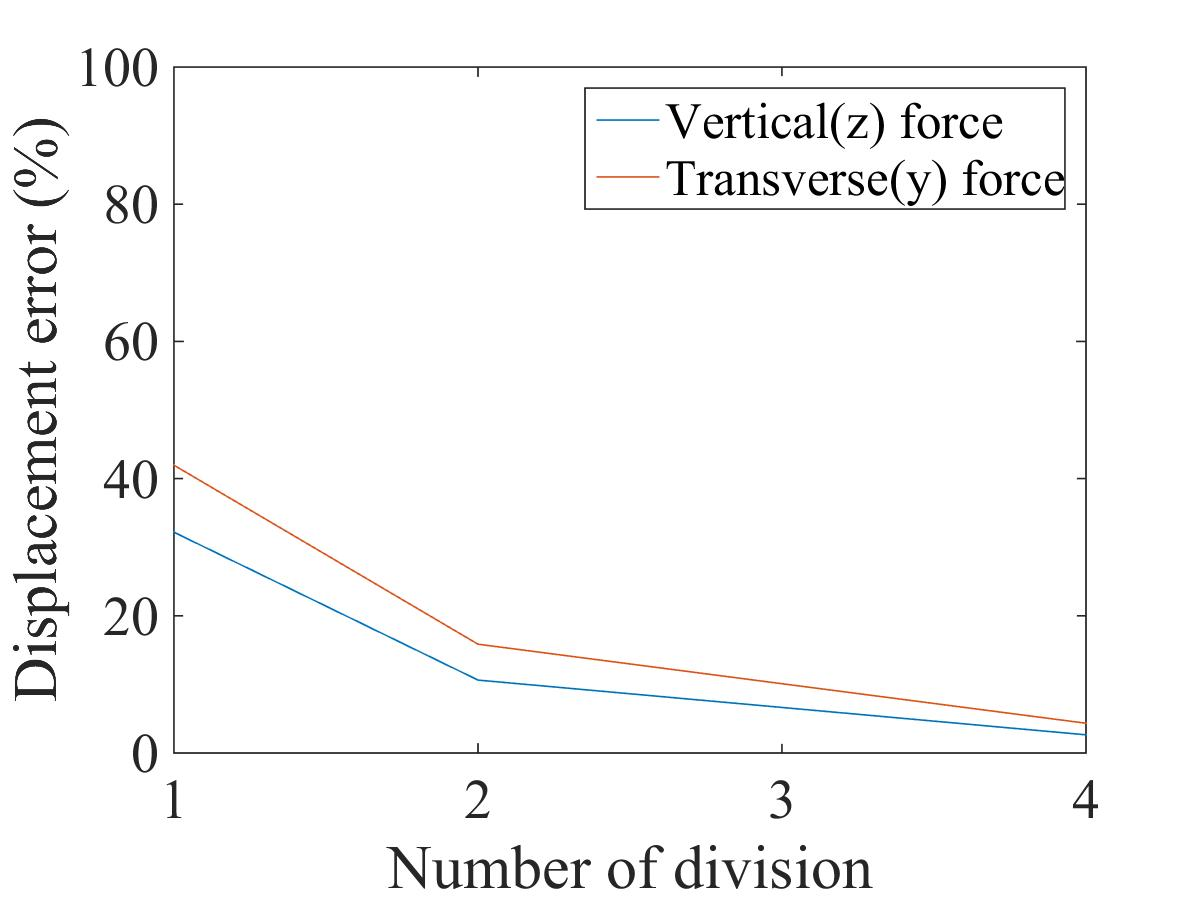
\includegraphics[width=6cm]{../Figure-files/error8brick_beam_irregular_shape1100.jpeg}
  \captionsetup{justification=centering,margin=3cm}
  \caption{8NodeBrick cantilever beam for irregular \emph{\textbf{Shape 1}}\\
      Displacement error   versus   Number of division}
  % \caption{}
  \label{fig shape 1 8NodeBrick cantilever beam for irregular more elements}
\end{figure}


% \begin{figure}[H]
%   % \centering
%   \begin{subfigure}{0.5\textwidth}
%     \centering
%     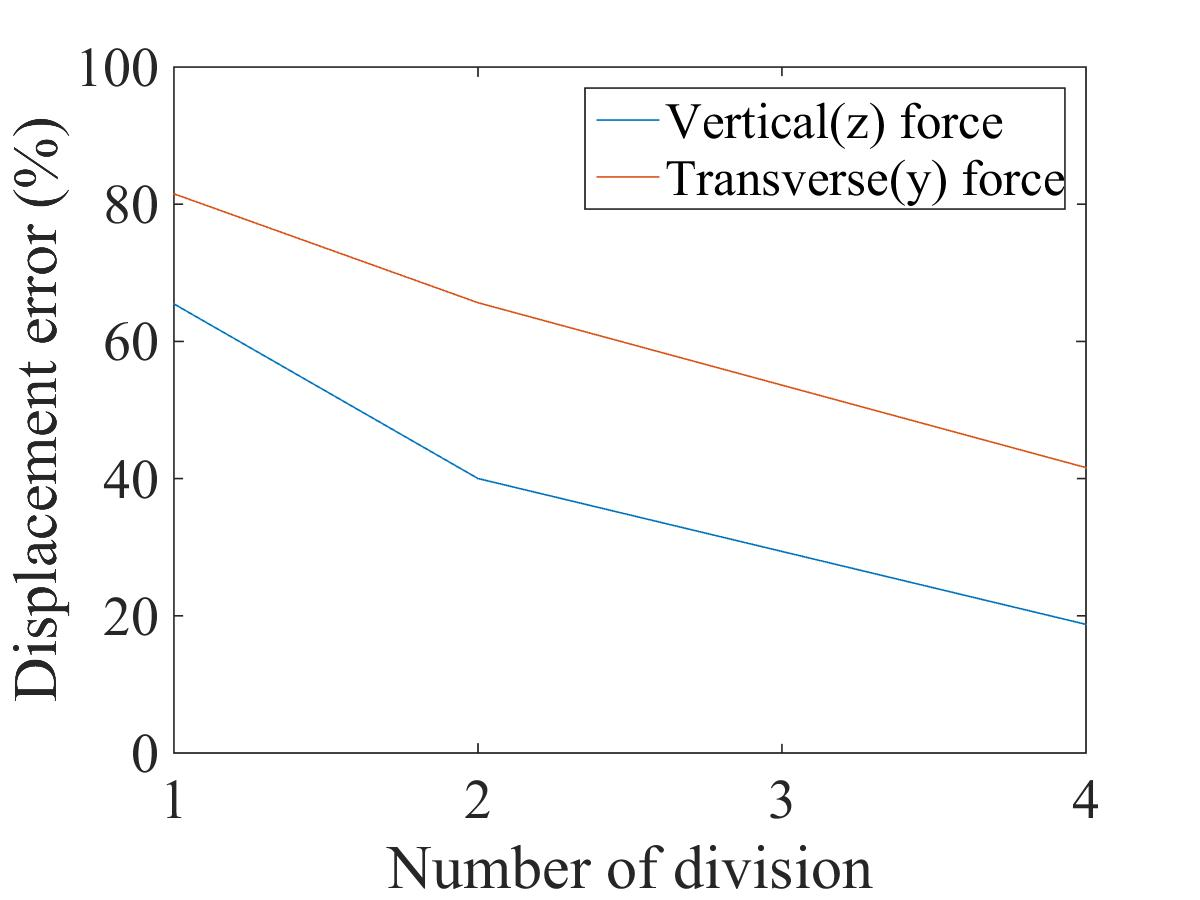
\includegraphics[width=6cm]{../Figure-files/error8brick_beam_irregular_shape2.jpeg}
%     \caption{Error scale 0\% - 80\%}
%   \end{subfigure}
%   \begin{subfigure}{0.5\textwidth}
%     \centering
%     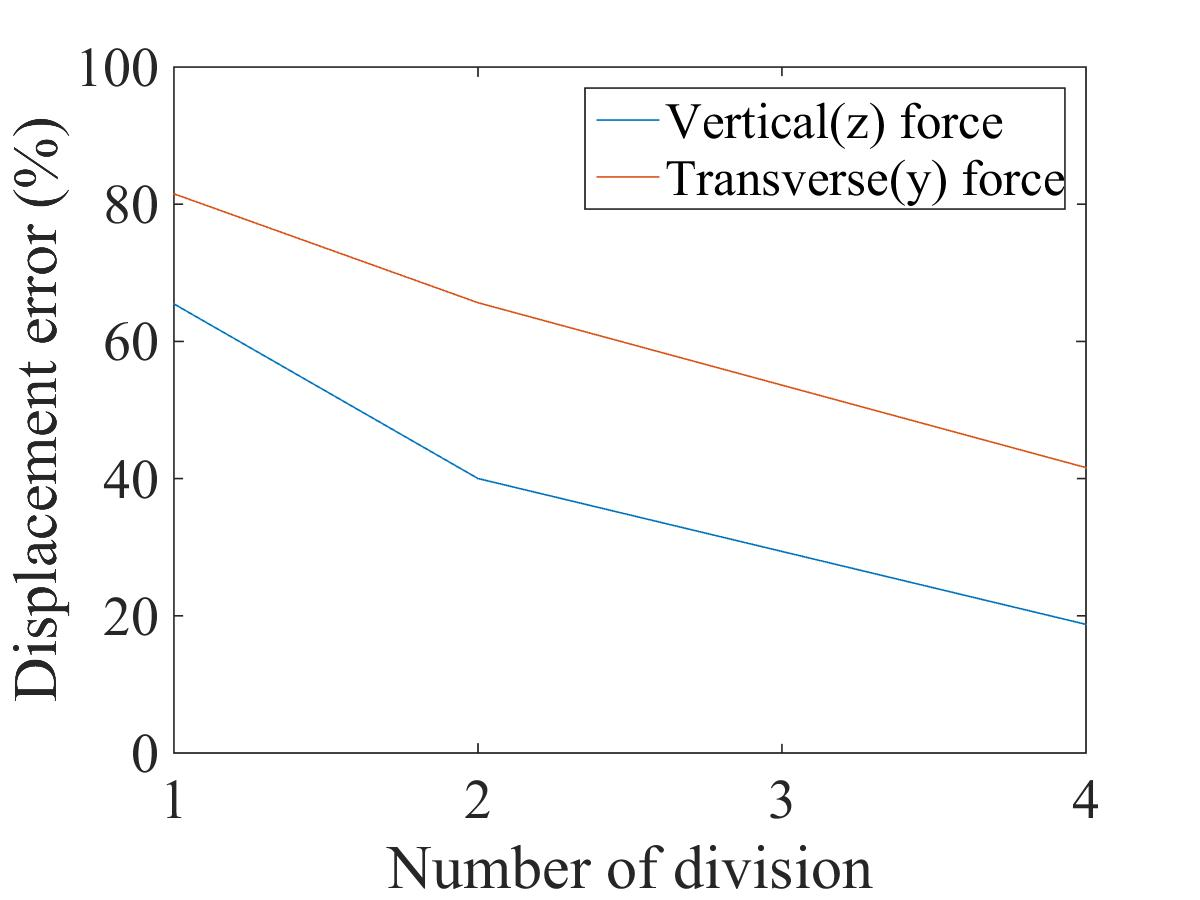
\includegraphics[width=6cm]{../Figure-files/error8brick_beam_irregular_shape2100.jpeg}
%     \caption{Error scale 0\% - 100\%}
%   \end{subfigure}
%   \captionsetup{justification=centering,margin=3cm}
%   \caption{Two sub}
%   % \caption{}
%   % \label{}
% \end{figure}

\begin{figure}[H]
  % \centering
    \centering
    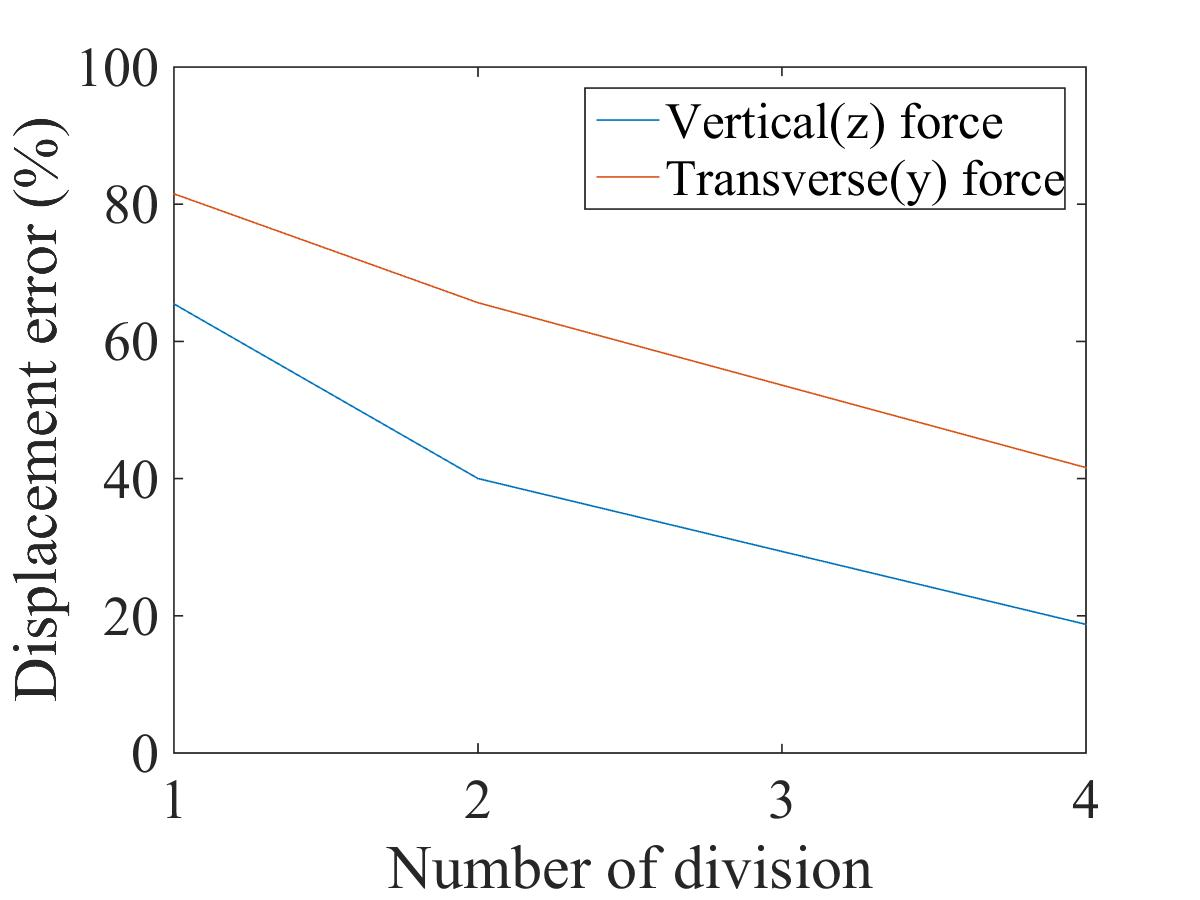
\includegraphics[width=6cm]{../Figure-files/error8brick_beam_irregular_shape2.jpeg}
  \captionsetup{justification=centering,margin=3cm}
  \caption{8NodeBrick cantilever beam for irregular \emph{\textbf{Shape 2}} \\
      Displacement error   versus   Number of division}
  % \caption{}
  \label{fig shape 2 8NodeBrick cantilever beam for irregular more elements}
\end{figure}



% \begin{figure}[H]
%   % \centering
%   \begin{subfigure}{0.5\textwidth}
%     \centering
%     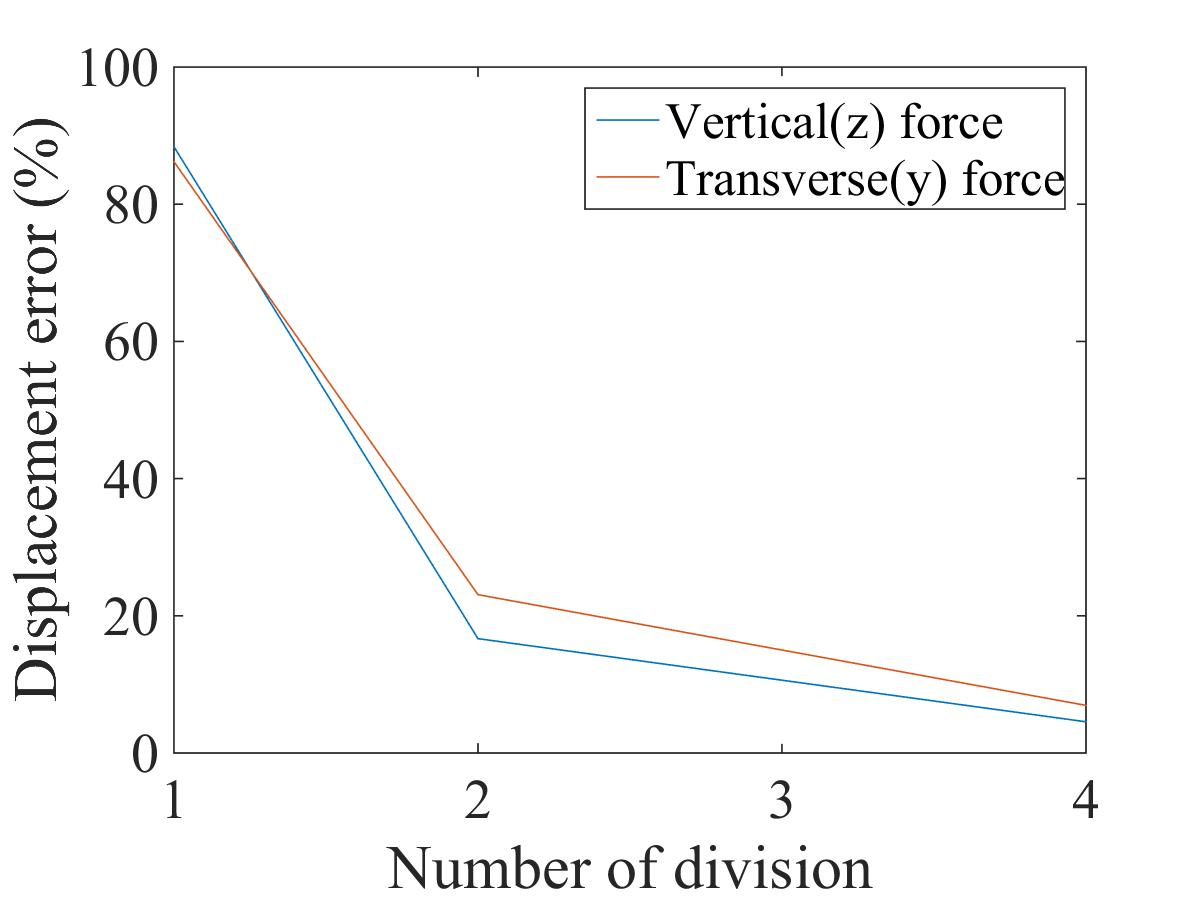
\includegraphics[width=6cm]{../Figure-files/error8brick_beam_irregular_shape3.jpeg}
%     \caption{Error scale 0\% - 80\%}
%   \end{subfigure}
%   \begin{subfigure}{0.5\textwidth}
%     \centering
%     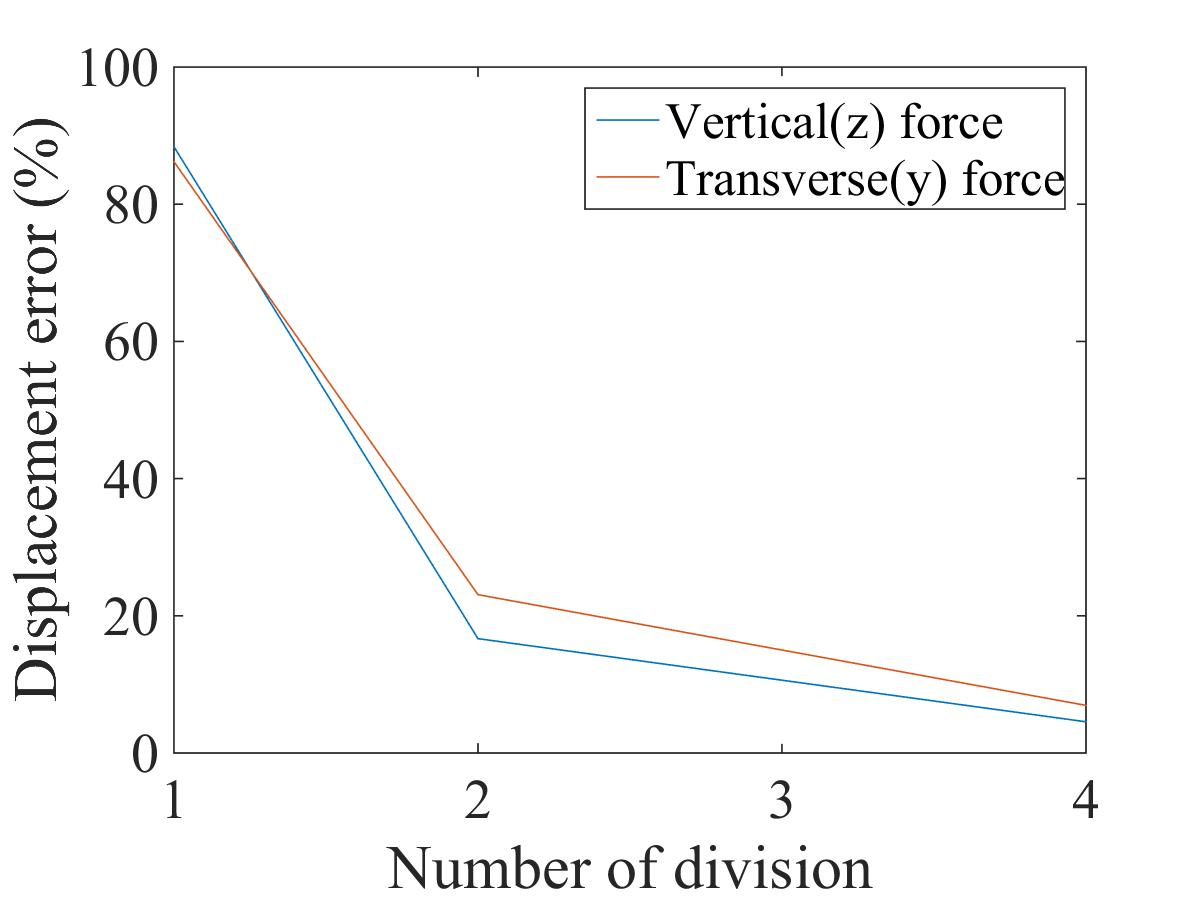
\includegraphics[width=6cm]{../Figure-files/error8brick_beam_irregular_shape3100.jpeg}
%     \caption{Error scale 0\% - 100\%}
%   \end{subfigure}
%   \captionsetup{justification=centering,margin=3cm}
%   \caption{Two sub}
%   % \caption{}
%   % \label{}
% \end{figure}

\begin{figure}[H]
  % \centering
    \centering
    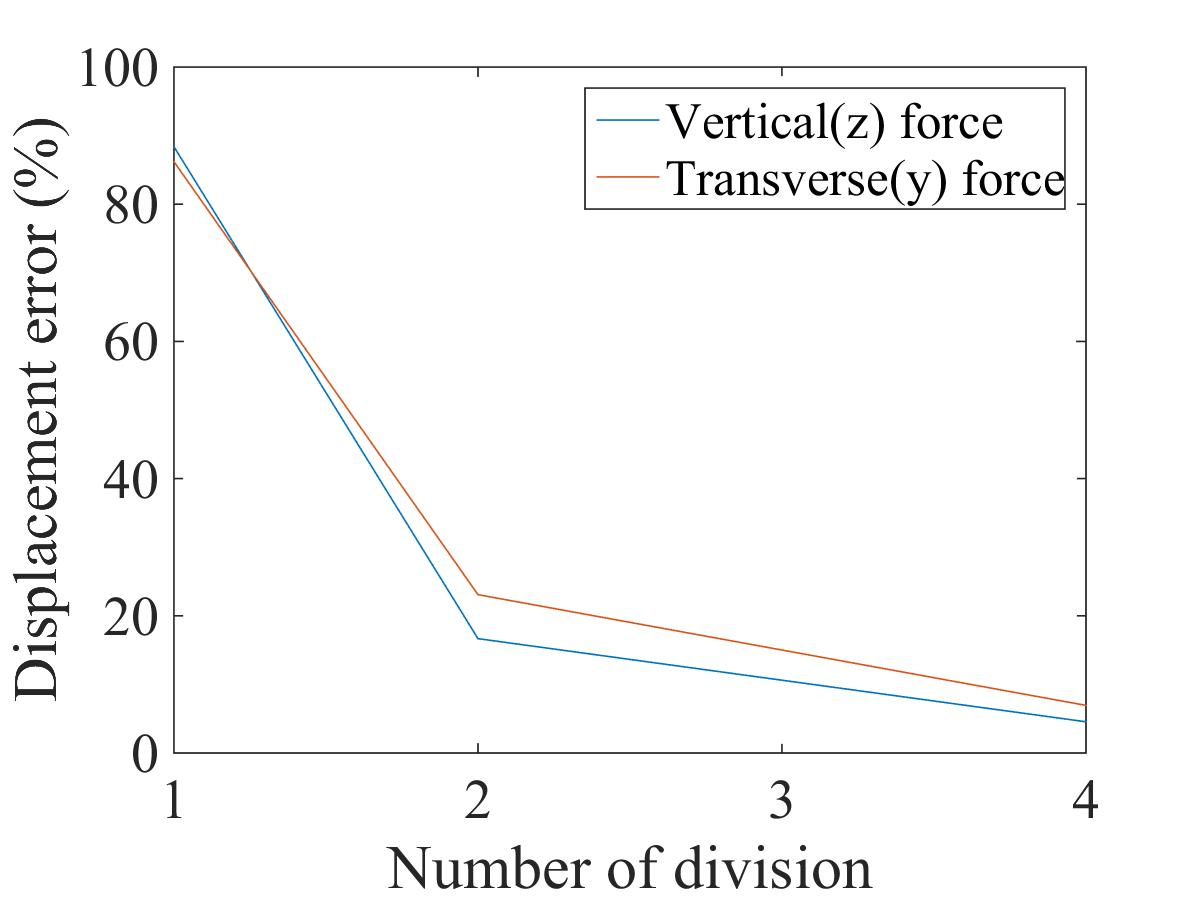
\includegraphics[width=6cm]{../Figure-files/error8brick_beam_irregular_shape3.jpeg}
  \captionsetup{justification=centering,margin=3cm}
  \caption{8NodeBrick cantilever beam for irregular \emph{\textbf{Shape 3}}\\
      Displacement error   versus   Number of division}
  % \caption{}
  \label{fig shape 3 8NodeBrick cantilever beam for irregular more elements}
\end{figure}



The ESSI model fei files for the table above are \href{https://github.com/yuan-energy/ESSI_Verification/blob/master/8NodeBrick/cantilever_irregular_element_cut/cantilever_irregular_element_cut.tar.gz?raw=true}{here}











% \newpage
% \subsection{Verification of 8NodeBrick edge clamped beams }

% Problem description: Length=6m, Width=1m, Height=1m, Force=100N, E=1E8Pa, $\nu=0.0$. Use the shear deformation coefficient $\kappa=1.2$. The force direction was shown in Figure (\ref{fig Problem description for clamped beams}). 

% \begin{figure}[H]
%   \centering
%   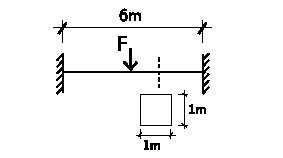
\includegraphics[width=7cm]{../Figure-files/clamped_beam.pdf}
%   \caption{Problem description for clamped beams}
%   \label{fig Problem description for clamped beams}
% \end{figure}

% % \subsection{Verification of edge clamped beams - one line elements}



% The elment types and element sizes were same to the cantilever model. Only the boundary conditions and external force locations were changed. 

% Numerical model:

% The 8NodeBrick elements were shown in Figure (\ref{fig 8NodeBrick elements for clamped beams}).

% \begin{figure}[H]
%   \centering
%   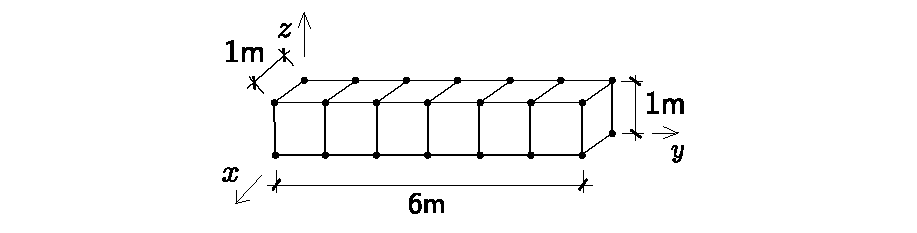
\includegraphics[width=9cm]{../Figure-files/beam_8brick.pdf}
%   \caption{8NodeBrick elements for clamped beams}
%   \label{fig 8NodeBrick elements for clamped beams}
% \end{figure}

% Theoretical displacement (bending and shear deformation):
% \begin{equation}
%   \begin{aligned}
%   d &=\frac{FL^3}{192EI}+\frac{\frac{F}{2}\frac{L}{2}}{GA_v}  \\
%     &=\frac{FL^3}{192E\frac{bh^3}{12}}+\frac{\frac{F}{2}\frac{L}{2}}{\frac{E}{2(1+\nu)}\frac{bh}{\kappa}} \\
%    &= \frac{100 N\times 6 m^3}{192 \times 10^8 N/m^2 \times \frac{1}{12} m^4}+ 
%     \frac{\frac{100}{2} N \times \frac{6}{2} m}{\frac{10}{2}\times 10^7 N/m^2\times 1 m^2\times \frac{5}{6}}   \\
%   &=1.35\times 10^{-5} m + 0.36\times 10^{-5} m  \\
%   &=1.71\times 10^{-5} \ m 
%     \end{aligned}
% \end{equation}

% The theoretical solution for $L=6\ m$ was calculated above, while the solutions for other length were calculated by the similar process. 

% In the figures above, only the model with geometry $6m\times 1m \times 1m$ was drawed. In the ESSI models, the geometry $10m\times 1m \times 1m$ and the geometry $20m\times 1m \times 1m$ were also calculated. In three different geometry models, all the element sizes were $1m\times 1m \times 1m$. Therefore, the number of elements used in each model were $6,\ 10\ and\ 20$ respectively.

% The results were listed in Table (\ref{table Results for 8NodeBrick clamped beams of different geometry}).

% \begin{table}[H]
%   \centering
%     \caption{Results for 8NodeBrick clamped beams of different geometry}
%     \label{table Results for 8NodeBrick clamped beams of different geometry}
%     \begin{tabular}{|c|c|c|c|c|c|}
%     \hline
%     Geometry & 8NodeBrick & Theory(bending) & Theory(shear) & Theory(all) & Error   \\  \hline
%     1:6      & 1.100E-05 $m$ & 1.35E-05  $m$     & 2.50E-06  $m$   & 1.60E-05 $m$        & 33.33\% \\ \hline
%     1:10     & 4.500E-05 $m$ & 6.25E-05  $m$     & 5.00E-06  $m$   & 6.75E-05 $m$        & 33.33\% \\ \hline
%     1:20     & 3.400E-04 $m$ & 5.00E-04  $m$     & 1.00E-05  $m$   & 5.10E-04 $m$        & 33.33\% \\
%     \hline
%     \end{tabular}
% \end{table}

% The ESSI model fei files for the table above are \href{https://github.com/yuan-energy/ESSI_Verification/blob/master/8NodeBrick/clamped_beam_different_geometry/clamped_beam_different_geometry.tar.gz?raw=true}{here}





% 
% old table : may be useful.....
% \begin{table}[H]
%   \centering
%   \begin{tabular}{|c|c|c|c|c|}
%     \hline 
%     \multicolumn{5}{|c|}{The edge clamped beam displacement errors}   \\ \hline
%     Element Type  & Force direction  &1:6 & 1:10 & 1:20  \\ \hline 
%     4NodeANDES & in-plane       &    &   & \\ \hline
%     4NodeANDES & out-of-plane        &    &   &  \\ \hline
%     \multicolumn{2}{|c|}{8NodeBrick} &    &   &  \\ \hline
%     \multicolumn{2}{|c|}{27NodeBrick} &   &   &  \\ \hline
%   \end{tabular}
%   % \caption{}
% \end{table}




\newpage
In this section, the beam was cut into smaller elements with element side length 0.5m and 0.25m respectively. And the element side length of the original models is 1.0m. The numerical models were shown in Figure (\ref{fig 8NodeBrick clamped beams with element side length 1.0m}), (\ref{fig 8NodeBrick clamped beams with element side length 0.5m}) and (\ref{fig 8NodeBrick clamped beams with element side length 0.25m}). 

Number of division 1:

\begin{figure}[H]
  \centering
  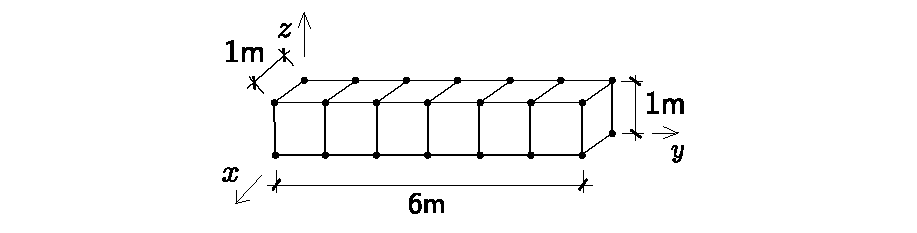
\includegraphics[width=9cm]{../Figure-files/beam_8brick.pdf}
  \caption{8NodeBrick clamped beams with element side length 1.0m}
  \label{fig 8NodeBrick clamped beams with element side length 1.0m}
\end{figure}

Number of division 2:

\begin{figure}[H]
  \centering
  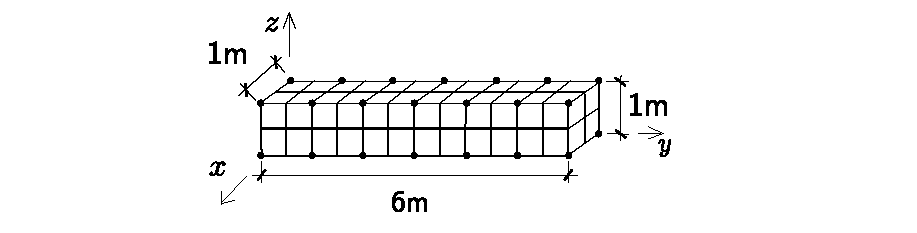
\includegraphics[width=9cm]{../Figure-files/beam_8brick_more_2.pdf}
  \caption{8NodeBrick clamped beams with element side length 0.5m}
  \label{fig 8NodeBrick clamped beams with element side length 0.5m}
\end{figure}

Number of division 4:

\begin{figure}[H]
  \centering
  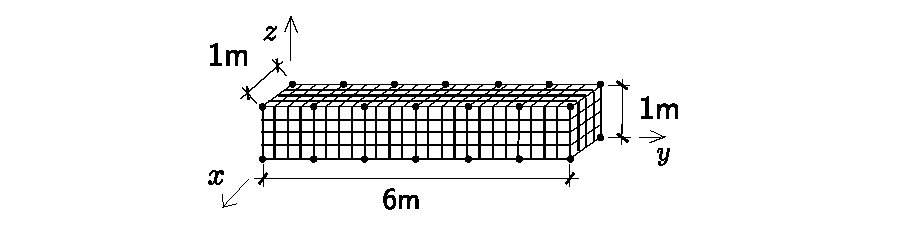
\includegraphics[width=9cm]{../Figure-files/beam_8brick_more.pdf}
  \caption{8NodeBrick clamped beams with element side length 0.25m}
  \label{fig 8NodeBrick clamped beams with element side length 0.25m}
\end{figure}


The ESSI results were listed in Table (\ref{table Results for 8NodeBrick clamped beams with more elements}). 
The theoretical solution is 1.60E-5 $m$. 

\begin{table}[H]
  \centering
  \caption{Results for 8NodeBrick clamped beams with more elements}
  \label{table Results for 8NodeBrick clamped beams with more elements}
  \begin{tabular}{|c|c|c|c|c|}
    \hline 
    \multirow{2}{*}{Element Type} 
       & \multicolumn{3}{|c|}{Element side length} \\ \cline{2-4}
       & 1 $m$ & 0.5 $m$ & 0.25 $m$ \\                              \hline
8NodeBrick & 1.10E-05 $m$ & 1.47E-05 $m$ & 1.64E-05 $m$ \\ \hline
Error      & 33.33\%  & 11.09\%  & 0.73\%   \\ \hline
  \end{tabular}
  % \caption{}
\end{table}

The errors were plotted in Figure (\ref{fig error 8NodeBrick clamped beam for different element number}).

\begin{figure}[H]
  % \centering
  \begin{subfigure}{0.5\textwidth}
    \centering
    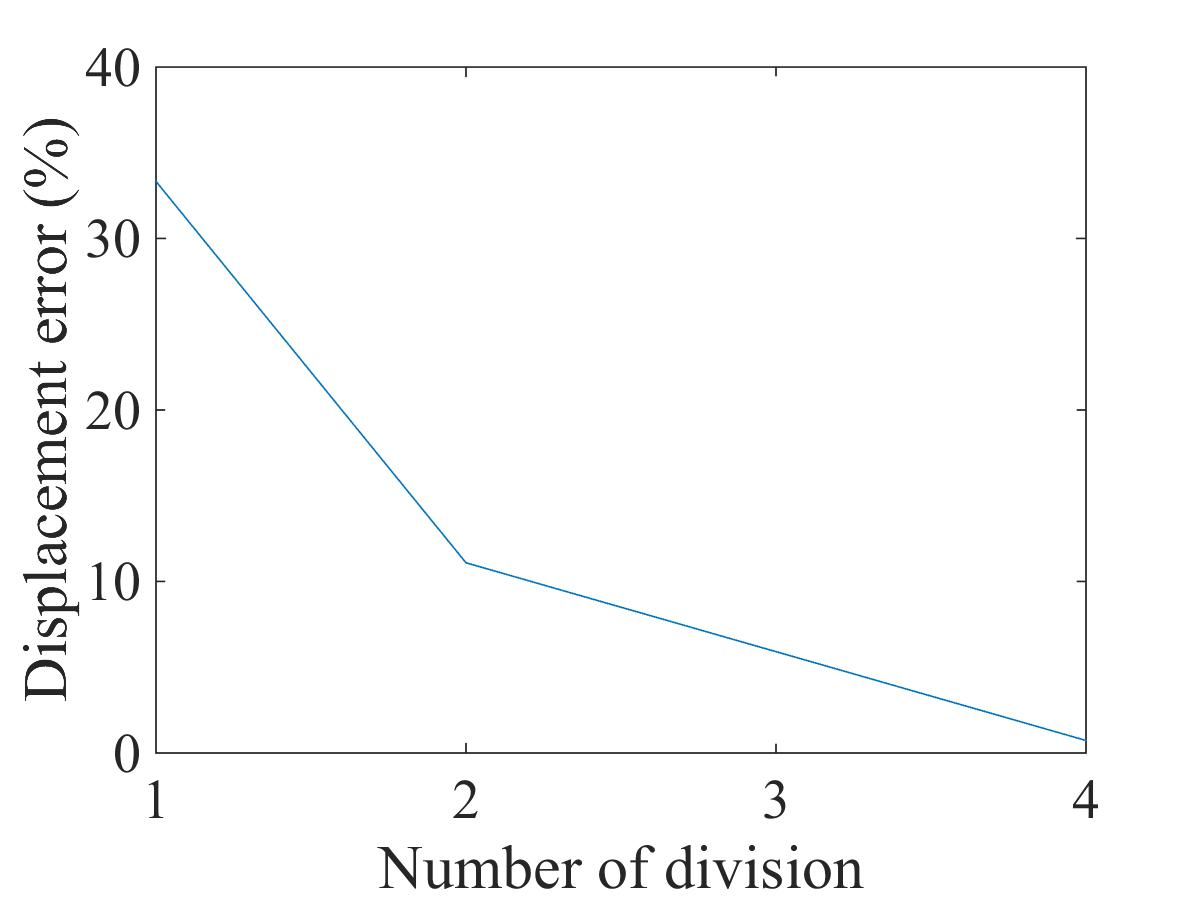
\includegraphics[width=6cm]{../Figure-files/error8brick_clamped_beam_diff_element.jpeg}
    \caption{Error scale 0\% - 40\%}
  \end{subfigure}
  \begin{subfigure}{0.5\textwidth}
    \centering
    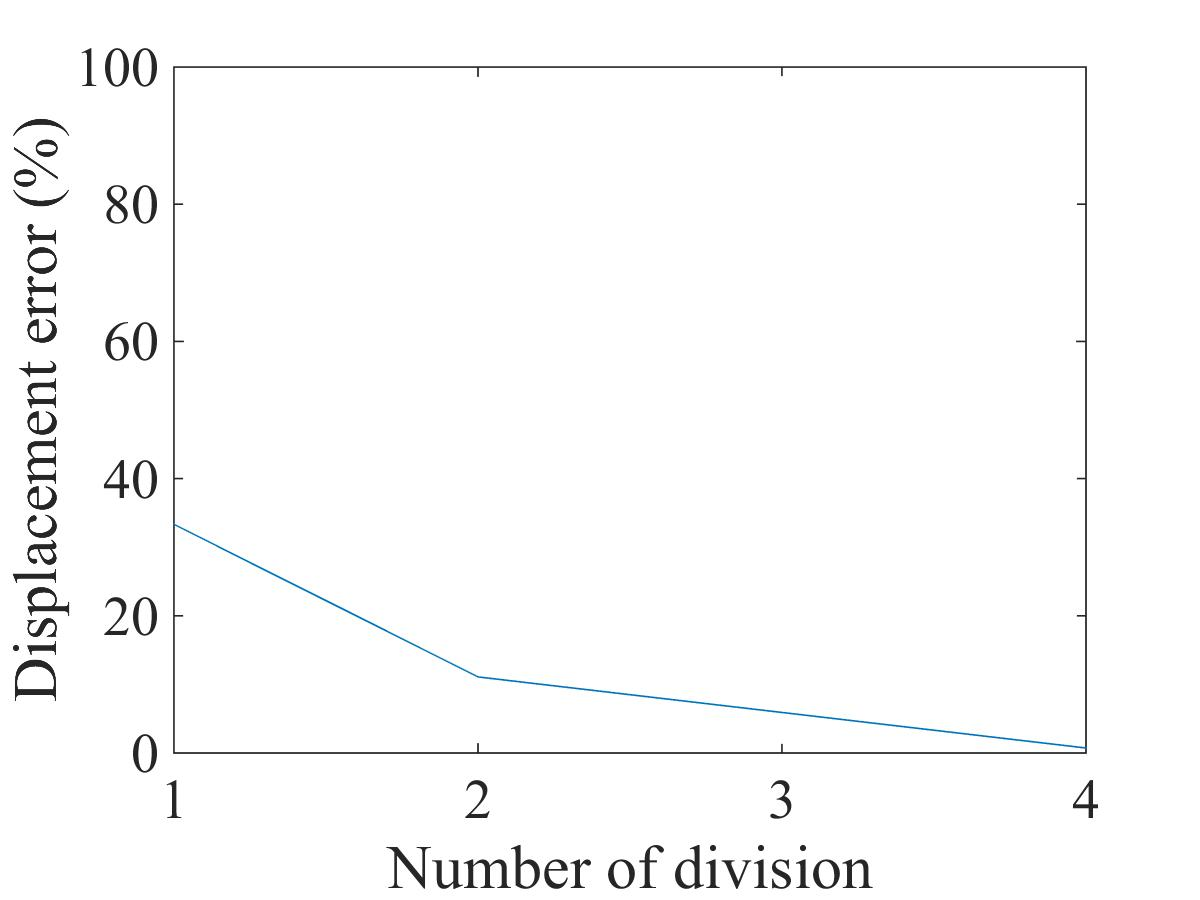
\includegraphics[width=6cm]{../Figure-files/error8brick_clamped_beam_diff_element100.jpeg}
    \caption{Error scale 0\% - 100\%}
  \end{subfigure}
  \captionsetup{justification=centering,margin=3cm}
  \caption{8NodeBrick clamped beam for different element number\\
      Displacement error   versus   Number of division}
  \label{fig error 8NodeBrick clamped beam for different element number}
\end{figure}


The ESSI model fei files for the table above are \href{https://github.com/yuan-energy/ESSI_Verification/blob/master/8NodeBrick/clamped_beam_cut/clamped_beam_cut.tar.gz?raw=true}{here}








\newpage
\subsection{Verification of 8NodeBrick stress in cantilever beams}





Problem description: Length=6m, Width=1m, Height=1m, Force=100N, E=1E8Pa, $\nu=0.0$. Use the shear deformation coefficient $\kappa=1.2$. The force direction was shown in Figure (\ref{fig Problem description for cantilever beams of stress verification}). 

\begin{figure}[H]
  \centering
  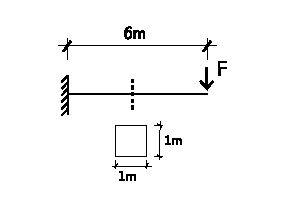
\includegraphics[width=7cm]{../Figure-files/cantilever_6.pdf}
  \caption{Problem description for cantilever beams of stress verification}
  \label{fig Problem description for cantilever beams of stress verification}
\end{figure}

The theoretical solution for the stress was calculated below. 

The 8NodeBrick elements were shown in Figure (\ref{fig 8NodeBrick for cantilever beams of stress verification}).
\begin{figure}[H]
  \centering
  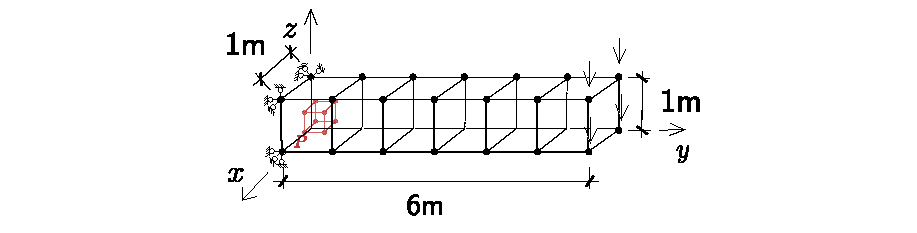
\includegraphics[width=9cm]{../Figure-files/beam_8brick_6div_gp.pdf}
  \caption{8NodeBrick for cantilever beams of stress verification}
  \label{fig 8NodeBrick for cantilever beams of stress verification}
\end{figure}

The bending moment at the Gassian Point is 
\begin{equation}
  M=F(L-P_y)=100 N \times (6-0.2113) m = 578.87 N\cdot m
\end{equation}

The bending modulus is 
\begin{equation}
  I= \frac{bh^3}{12}=\frac{1}{12} m^4
\end{equation}

Therefore, the theoretical stress is 
\begin{equation}
  \sigma= \frac{M\cdot z}{I}= \frac{578.87 N\cdot m \times (0.5-0.2113) m }{\frac{1}{12} m^4}= 2005 Pa
\end{equation}



To get a better result, the same geometry beam was also cut into small elements. When more elements were used, the theoretical stress was calculated again with the new coordinates. The calculation process is similar to the process above. 

The numerical models were shown in Figure (\ref{fig 8NodeBrick stress with element side length 1.0m}), (\ref{fig 8NodeBrick stress with element side length 0.5m}) and (\ref{fig 8NodeBrick stress with element side length 0.25m}). 


Number of division 1:

\begin{figure}[H]
  \centering
  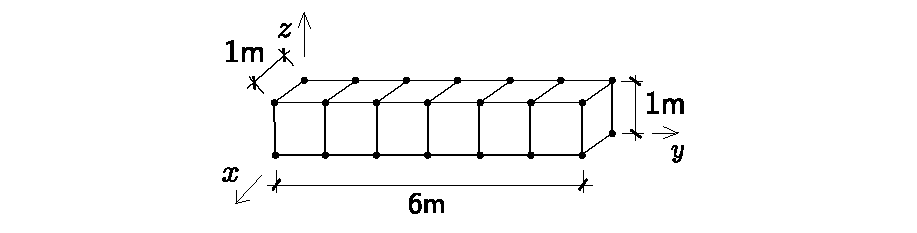
\includegraphics[width=9cm]{../Figure-files/beam_8brick.pdf}
  \caption{8NodeBrick stress with element side length 1.0m}
  \label{fig 8NodeBrick stress with element side length 1.0m}
\end{figure}

Number of division 2:

\begin{figure}[H]
  \centering
  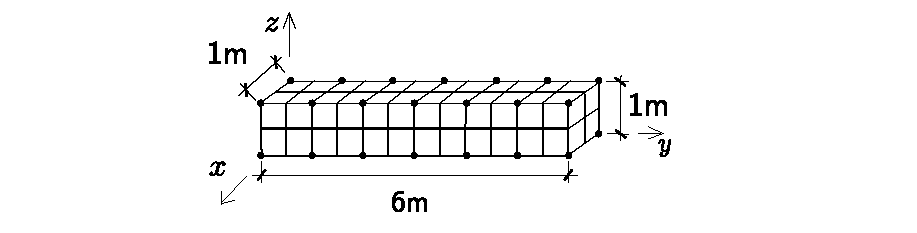
\includegraphics[width=9cm]{../Figure-files/beam_8brick_more_2.pdf}
  \caption{8NodeBrick stress with element side length 0.5m}
  \label{fig 8NodeBrick stress with element side length 0.5m}
\end{figure}

Number of division 4:

\begin{figure}[H]
  \centering
  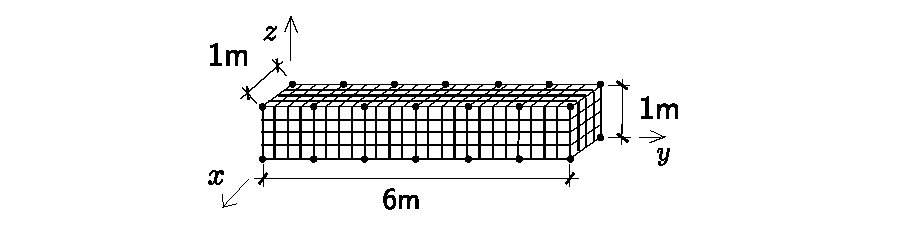
\includegraphics[width=9cm]{../Figure-files/beam_8brick_more.pdf}
  \caption{8NodeBrick stress with element side length 0.25m}
  \label{fig 8NodeBrick stress with element side length 0.25m}
\end{figure}


All the stress results were listed in Table (\ref{table Results for 8NodeBrick stress with more elements}). 


\begin{table}[H]
  \centering
  \caption{Results for 8NodeBrick stress with more elements}
  \label{table Results for 8NodeBrick stress with more elements}
  \begin{tabular}{|c|c|c|c|c|}
    \hline 
    \multirow{2}{*}{Element Type} 
       & \multicolumn{3}{|c|}{Element side length} \\ \cline{2-4}
       & 1 $m$ & 0.5 $m$ & 0.25 $m$ \\                              \hline
8NodeBrick & 1270.17 $Pa$ & 2418.60 $Pa$ & 3085.48 $Pa$ \\ \hline
Theoretical & 2005.26 $Pa$ & 2789.23 $Pa$ & 3191.27 $Pa$ \\ \hline
Error      & 36.66\% & 13.29\% & 3.31\%  \\ \hline
  \end{tabular}
  % \caption{}
\end{table}

The errors were plotted in Figure (\ref{fig 8NodeBrick cantilever beams for stress verification}).
\begin{figure}[H]
  % \centering
  \begin{subfigure}{0.5\textwidth}
    \centering
    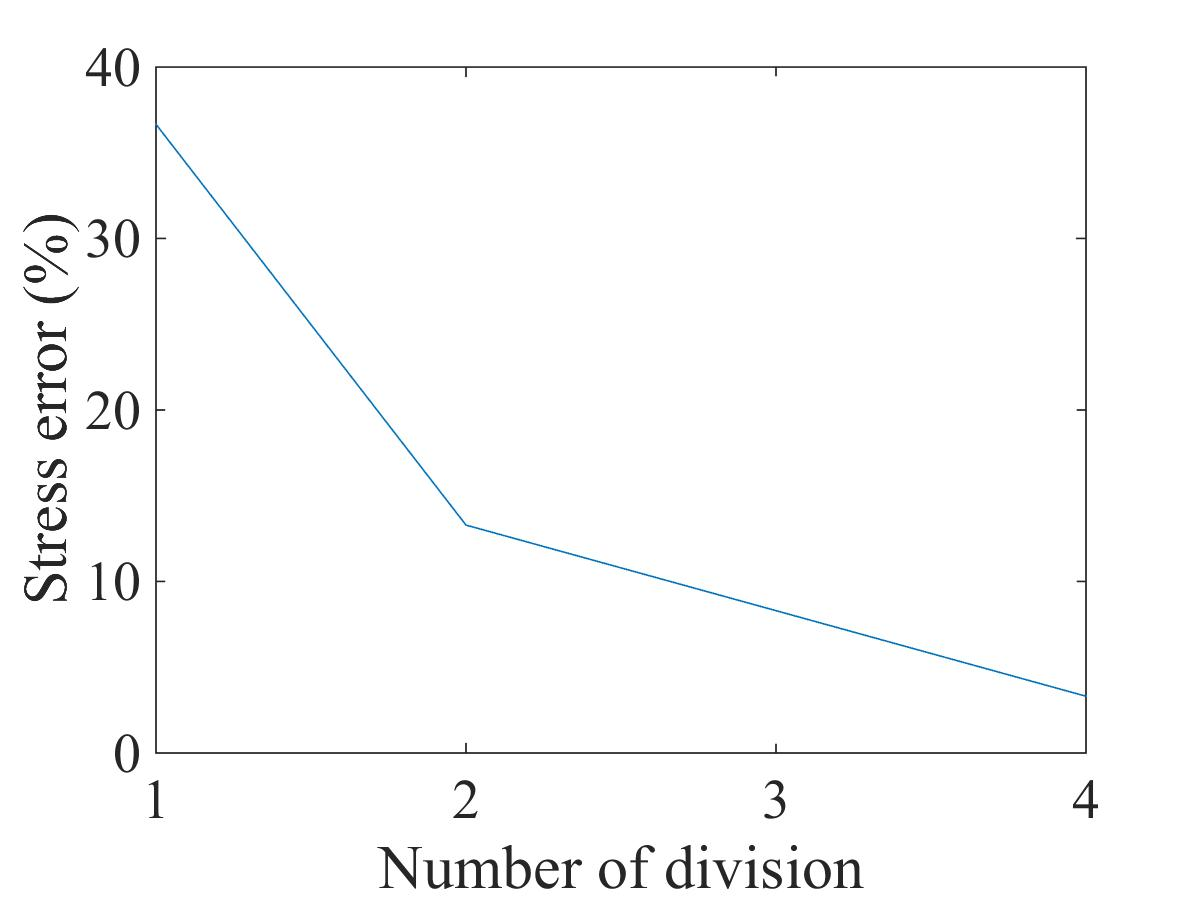
\includegraphics[width=6cm]{../Figure-files/error8brick_beam_stress.jpeg}
    \caption{Error scale 0\% - 40\%}
  \end{subfigure}
  \begin{subfigure}{0.5\textwidth}
    \centering
    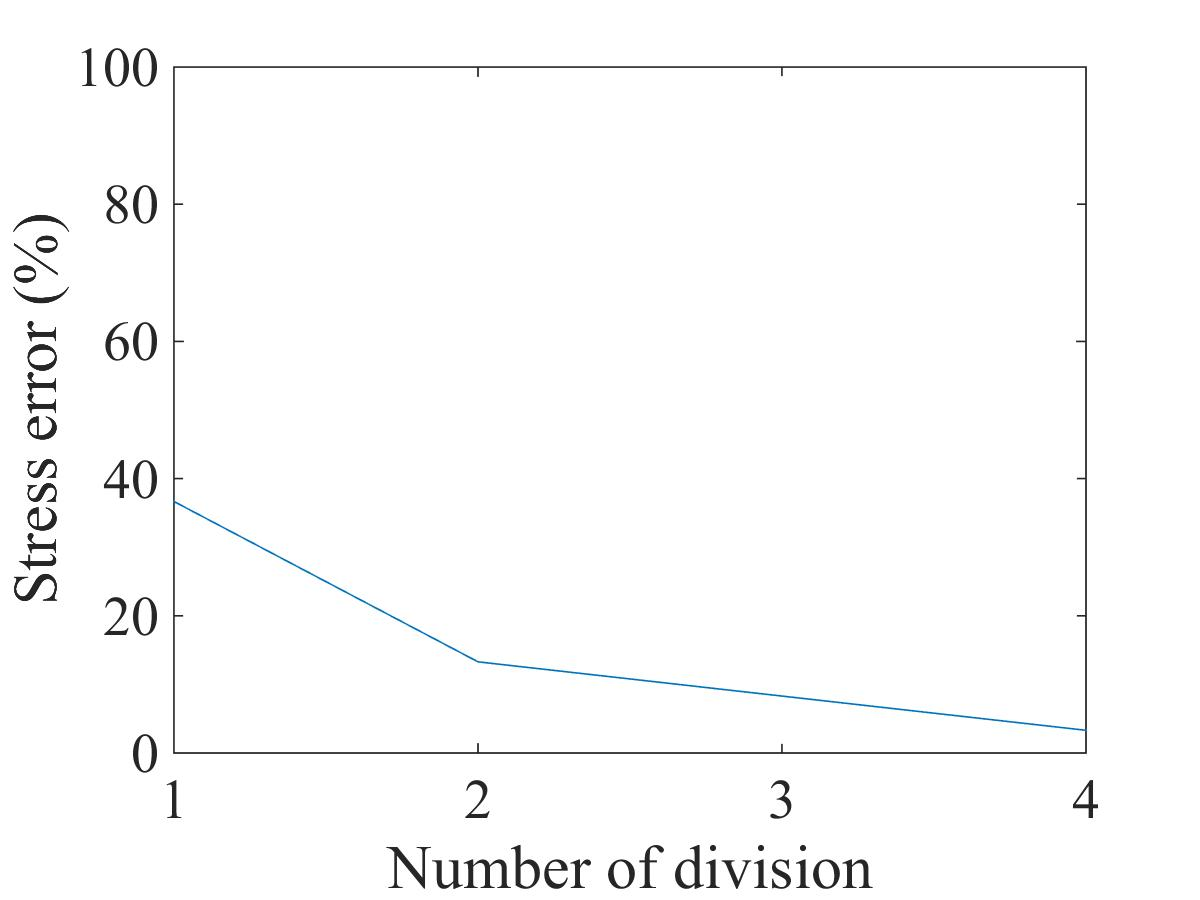
\includegraphics[width=6cm]{../Figure-files/error8brick_beam_stress100.jpeg}
    \caption{Error scale 0\% - 100\%}
  \end{subfigure}
  \captionsetup{justification=centering,margin=3cm}
  \caption{8NodeBrick cantilever beams for stress verification\\
      Stress error   versus   Number of division}
  \label{fig 8NodeBrick cantilever beams for stress verification}
\end{figure}


The ESSI model fei files for the table above are \href{https://github.com/yuan-energy/ESSI_Verification/blob/master/8NodeBrick/cantilever_stress/cantilever_stress.tar.gz?raw=true}{here}




\newpage
\subsection{Verification of 8NodeBrick square plate with four edges clamped}

Problem description: Length=20m, Width=20m, Height=1m, Force=100N, E=1E8Pa, $\nu=0.3$. 

The four edges are clamped. 

The load is the uniform normal pressure on the whole plate. 


The plate flexural rigidity is 
\begin{equation}
  D=\frac{Eh^3}{12(1-\nu^2)}=\frac{10^8 N/m^2 \times 1^3 m^3 }{12 \times (1-0.3^2) }= 9.1575 \times 10^6 \ N\cdot m
\end{equation}
The theoretical solution is 
\begin{equation}
  d=\alpha_c \frac{q a^4}{D}=0.00406\times \frac{100 N/m^2 \times 20^4 m^4}{9.1575 \times 10^6 \ N\cdot m}=2.2015\times 10^{-3} m
\end{equation}

where $\alpha_c$ is a coefficient, which depends on the ratio of plate length to width. In this problem, the coefficient\footnote{Stephen Timoshenko, Theory of plates and shells (2nd edition). MrGRAW-Hill Inc, page120, 1959.} $\alpha_c$ is 0.00406.


The 8NodeBrick were shown in Figure (\ref{fig 8NodeBrick edges clamped square plate with element side length 10m }) - (\ref{fig 8NodeBrick edges clamped square plate with element side length 0.25m }). 


\begin{figure}[H]
  \centering
  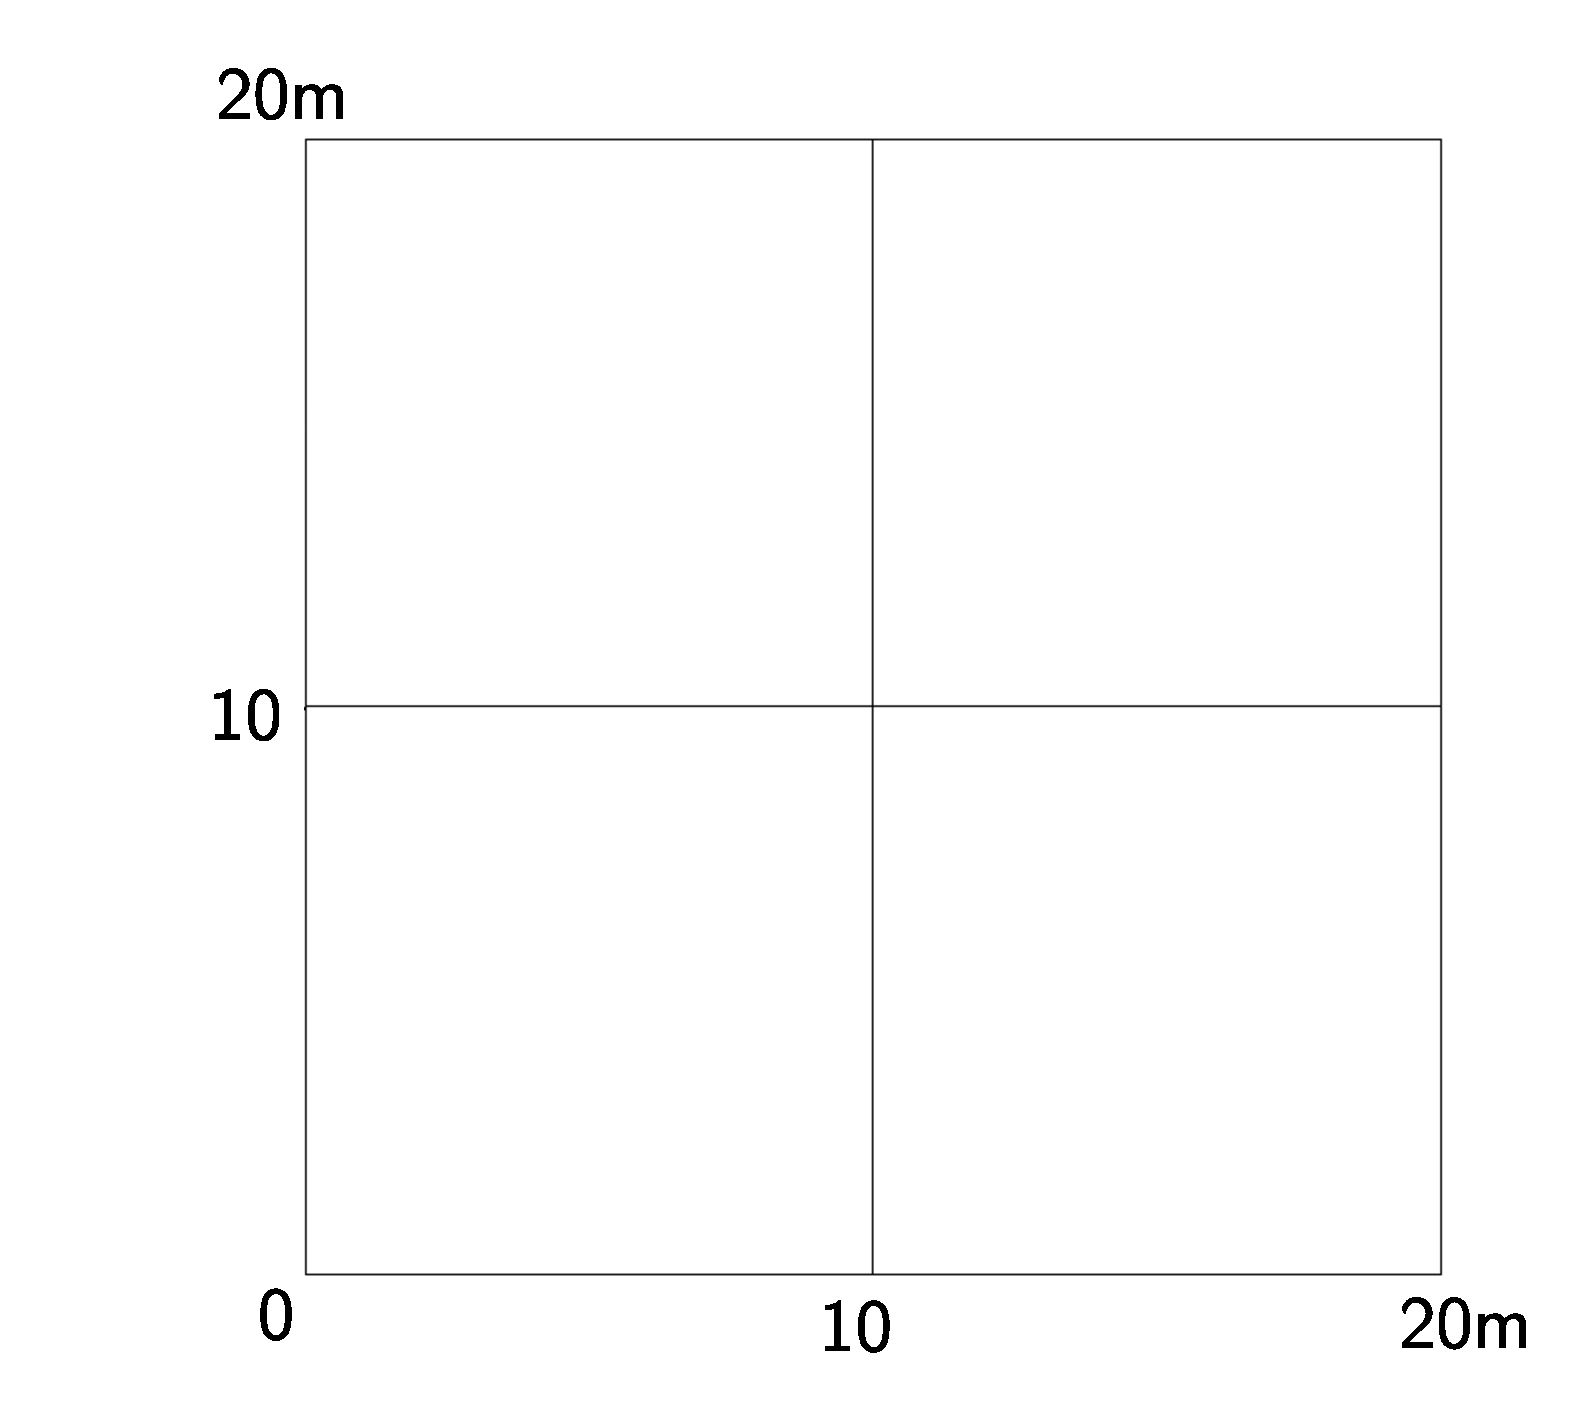
\includegraphics[width=11cm]{../Figure-files/square_plate1.pdf}
  \caption{8NodeBrick edge clamped square plate with element side length 10m }
  \label{fig 8NodeBrick edges clamped square plate with element side length 10m }
\end{figure}

\newpage

\begin{figure}[H]
  \centering
  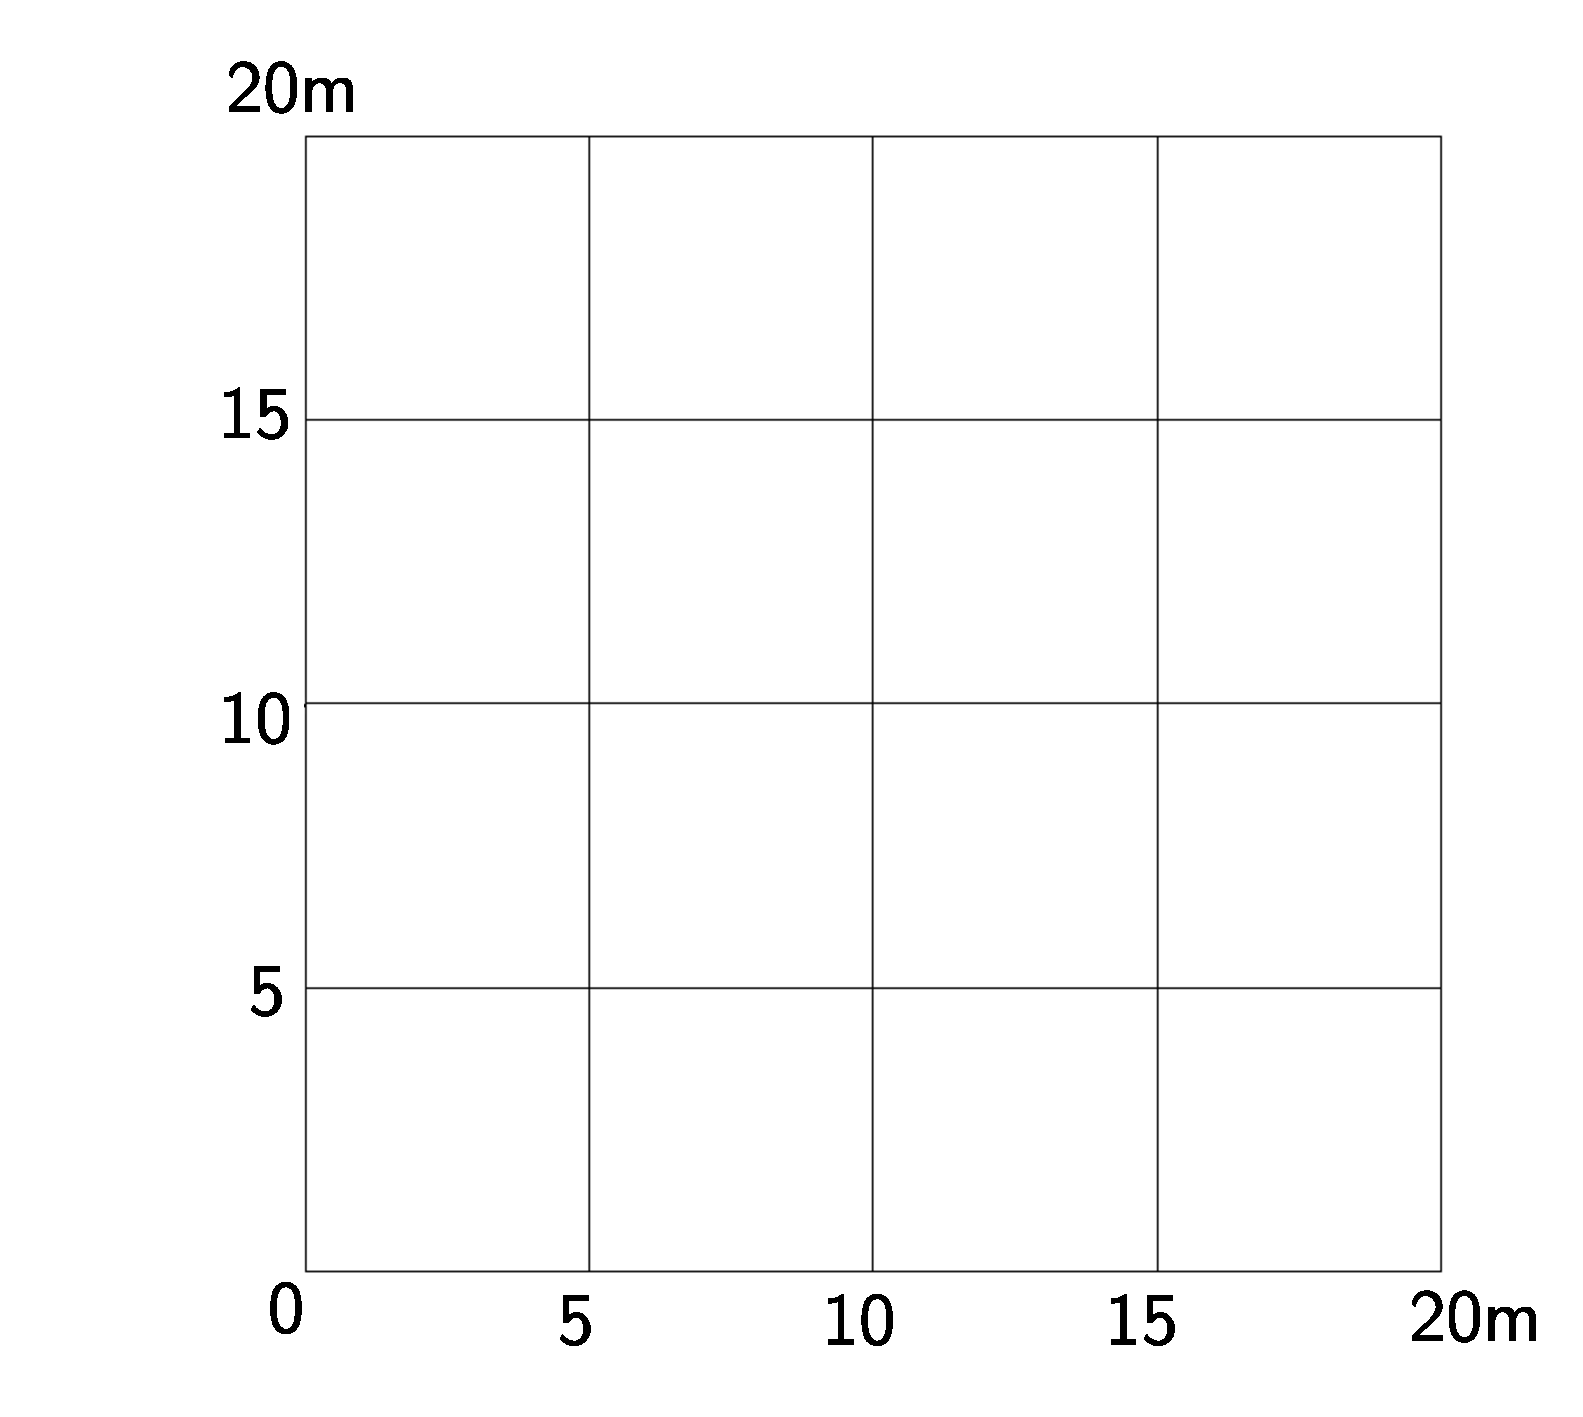
\includegraphics[width=11cm]{../Figure-files/square_plate2.pdf}
  \caption{8NodeBrick edge clamped square plate with element side length 5m }
  \label{fig 8NodeBrick edges clamped square plate with element side length 5m }
\end{figure}


\begin{figure}[H]
  \centering
  \includegraphics[width=11cm]{../Figure-files/square_plate3.pdf}
  \caption{8NodeBrick edge clamped square plate with element side length 2m }
  \label{fig 8NodeBrick edges clamped square plate with element side length 2m }
\end{figure}

\newpage

\begin{figure}[H]
  \centering
  \includegraphics[width=11cm]{../Figure-files/square_plate4.pdf}
  \caption{8NodeBrick edge clamped square plate with element side length 1m }
  \label{fig 8NodeBrick edges clamped square plate with element side length 1m }
\end{figure}


\begin{figure}[H]
  \centering
  \includegraphics[width=11cm]{../Figure-files/square_plate5.pdf}
  \caption{8NodeBrick edge clamped square plate with element side length 0.5m }
  \label{fig 8NodeBrick edges clamped square plate with element side length 0.5m }
\end{figure}

\newpage

\begin{figure}[H]
  \centering
  \includegraphics[width=11cm]{../Figure-files/square_plate6.pdf}
  \caption{8NodeBrick edge clamped square plate with element side length 0.25m }
  \label{fig 8NodeBrick edges clamped square plate with element side length 0.25m }
\end{figure}



The results were listed in Table (\ref{table Results for 8NodeBrick square plate with four edges clamped}).

\begin{table}[H]
  \centering
  \caption{Results for 8NodeBrick square plate with four edges clamped}
  \label{table Results for 8NodeBrick square plate with four edges clamped}
\begin{tabular}{|c|c|c|c|c|}
\hline
Element type     & 8NodeBrick     & 8NodeBrick     & 8NodeBrick     &  \multirow{3}{*}{\tabincell{c}{Theoretical \\ displacement}} \\ \cline{1-4}
Number of layers & 1layer         & 2layers         & 4layers         &          \\ \cline{1-4}
Element side length & Height:1.00$m$ & Height:0.50$m$ & Height:0.25$m$ &          \\ \hline
10$m$            & 9.75E-05  $m$  & 9.75E-05  $m$  & 9.75E-05 $m$  & 2.20E-03 $m$ \\ \hline
5$m$             & 3.28E-04  $m$  & 3.32E-04  $m$  & 3.32E-04 $m$  & 2.20E-03 $m$ \\ \hline
2$m$             & 1.04E-03  $m$  & 1.10E-03  $m$  & 1.12E-03 $m$  & 2.20E-03 $m$ \\ \hline
1$m$             & 1.56E-03  $m$  & 1.74E-03  $m$  & 1.79E-03 $m$  & 2.20E-03 $m$ \\ \hline
0.5$m$           & 1.80E-03  $m$  & 2.30E-03  $m$  & 2.12E-03 $m$  & 2.20E-03 $m$ \\ \hline
0.25$m$          & 1.87E-03  $m$  & 2.14E-03  $m$  & 2.23E-03 $m$  & 2.20E-03 $m$ \\
\hline
\end{tabular}
\end{table}


The errors were listed in Table (\ref{table Errors for 8NodeBrick square plate with four edges clamped}).

\begin{table}[H]
  \centering
  \caption{Errors for 8NodeBrick square plate with four edges clamped}
  \label{table Errors for 8NodeBrick square plate with four edges clamped}
\begin{tabular}{|c|c|c|c|c|}
\hline
Element type     & 8NodeBrick     & 8NodeBrick     & 8NodeBrick      \\ \hline
Number of layers & 1layer         & 2layers         & 4layers          \\ \hline
Element side length & Height:1.00$m$ & Height:0.50$m$ & Height:0.25$m$  \\ \hline
10$m$            & 95.57\%        & 95.57\%        & 95.57\%        \\ \hline
5$m$             & 85.09\%        & 84.94\%        & 84.91\%        \\ \hline
2$m$             & 52.98\%        & 50.09\%        & 49.25\%        \\ \hline
1$m$             & 28.93\%        & 21.17\%        & 18.72\%        \\ \hline
0.5$m$           & 18.26\%        & 4.58\%         & 3.56\%         \\ \hline
0.25$m$          & 15.05\%        & 2.70\%         & 1.37\%         \\
\hline
\end{tabular}
\end{table}



% \begin{figure}[H]
%   % \centering
%   \begin{subfigure}{0.5\textwidth}
%     \centering
%     \includegraphics[width=6cm]{../Figure-files/error8brick_square_plate_clamped.jpeg}
%     \caption{Error scale 0\% - 80\%}
%   \end{subfigure}
%   \begin{subfigure}{0.5\textwidth}
%     \centering
%     \includegraphics[width=6cm]{../Figure-files/error8brick_square_plate_clamped100.jpeg}
%     \caption{Error scale 0\% - 100\%}
%   \end{subfigure}
%   \captionsetup{justification=centering,margin=3cm}
%   \caption{Two sub}
%   % \caption{}
%   % \label{}
% \end{figure}


The errors were plotted in Figure (\ref{fig 8NodeBrick square plate with edge clamped}).
\begin{figure}[H]
  % \centering
    \centering
    \includegraphics[width=6cm]{../Figure-files/error8brick_square_plate_clamped.jpeg}
  \captionsetup{justification=centering,margin=3cm}
  \caption{8NodeBrick square plate with edge clamped\\
      Displacement error   versus   Number of side division}
  \label{fig 8NodeBrick square plate with edge clamped}
\end{figure}



The ESSI model fei files for the table above are \href{https://github.com/yuan-energy/ESSI_Verification/blob/master/8NodeBrick/square_plate_clamped/square_plate_clamped.tar.gz?raw=true}{here}




% \newpage
% \begin{itemize}
%   \item \textbf{\emph{Square plate with edges clamped: $100m \times 100m \times 1m$}}
% \end{itemize}

% The same verification procedures above were did for the square plate of $100m \times 100m \times 1m$. 

% The 








% \newpage
% \begin{itemize}
%   \item \textbf{\emph{Square plate with edges clamped: different geometry}}
% \end{itemize}

% In the figures above, only the model with geometry $20m\times 20m \times 1m$ was drawed. In the ESSI models, the geometry $6m\times 6m \times 1m$ and the geometry $10m\times 10m \times 1m$ were also calculated. In three different geometry models, all the element sizes were $1m\times 1m \times 1m$.


% The ESSI displacement results were listed below.

% \begin{table}[H]
%   \centering
%   \begin{tabular}{|c|c|c|c|c|c|}
%     \hline 
%     \multirow{2}{*}{Element Type}  & \multirow{2}{*}{Number of layers}   
%        &  \multicolumn{3}{|c|}{Model geometry} \\       \cline{3-5}
%        & & 1:6 & 1:10 & 1:20 \\                              \hline
% 8NodeBrick &  2layers   &2.13E-04 $m$ & 1.54E-03 $m$ & 2.41E-02 $m$  \\ \hline
% 8NodeBrick &  4layers   &2.37E-04 $m$ & 1.71E-03 $m$ & 2.66E-02 $m$  \\ \hline
% \multicolumn{2}{|c|}{Theoretical}    &1.78E-05 $m$ & 1.38E-04 $m$ & 2.20E-03 $m$      \\ \hline
%   \end{tabular}
%   % \caption{}
% \end{table}



% The errors were listed below.

% \begin{table}[H]
%   \centering
%   \begin{tabular}{|c|c|c|c|c|c|}
%     \hline 
%     \multirow{2}{*}{Element Type}  & \multirow{2}{*}{Number of layers}   
%        &  \multicolumn{3}{|c|}{Model geometry} \\       \cline{3-5}
%        & & 1:6 & 1:10 & 1:20 \\                              \hline
% 8NodeBrick &  2layers   &3.58\% & 9.47\% & 11.77\%  \\ \hline
% 8NodeBrick &  4layers   &7.27\% & 0.19\% & 2.66\%   \\ \hline
%   \end{tabular}
%   % \caption{}
% \end{table}












\newpage
\subsection{Verification of 8NodeBrick square plate with four edges simply supported}

Problem description: Length=20m, Width=20m, Height=1m, Force=100N, E=1E8Pa, $\nu=0.3$. 

The four edges are simply supported. 

The load is the uniform normal pressure on the whole plate. 

The plate flexural rigidity is 
\begin{equation}
  D=\frac{Eh^3}{12(1-\nu^2)}=\frac{10^8 N/m^2 \times 1^3 m^3 }{12 \times (1-0.3^2) }= 9.1575 \times 10^6 \ N\cdot m
\end{equation}
The theoretical solution is 
\begin{equation}
  d=\alpha_s \frac{q a^4}{D}=0.00126\times \frac{100 N/m^2 \times 20^4 m^4}{9.1575 \times 10^6 \ N\cdot m}=7.0936\times 10^{-3} m
\end{equation}

where $\alpha_s$ is a coefficient, which depends on the ratio of plate length to width. In this problem, the coefficient\footnote{Stephen Timoshenko, Theory of plates and shells (2nd edition). MrGRAW-Hill Inc, page202, 1959.} $\alpha_s$ is 0.00126.


The 8NodeBrick were shown in Figure (\ref{fig 8NodeBrick edges simply supported square plate with element side length 10m }) - (\ref{fig 8NodeBrick edges simply supported square plate with element side length 0.25m }). 



\begin{figure}[H]
  \centering
  \includegraphics[width=11cm]{../Figure-files/square_plate1.pdf}
  \caption{8NodeBrick edge simply supported square plate with element side length 10m }
  \label{fig 8NodeBrick edges simply supported square plate with element side length 10m }
\end{figure}

\newpage

\begin{figure}[H]
  \centering
  \includegraphics[width=11cm]{../Figure-files/square_plate2.pdf}
  \caption{8NodeBrick edge simply supported square plate with element side length 5m }
  \label{fig 8NodeBrick edges simply supported square plate with element side length 5m }
\end{figure}


\begin{figure}[H]
  \centering
  \includegraphics[width=11cm]{../Figure-files/square_plate3.pdf}
  \caption{8NodeBrick edge simply supported square plate with element side length 2m }
  \label{fig 8NodeBrick edges simply supported square plate with element side length 2m }
\end{figure}

\newpage

\begin{figure}[H]
  \centering
  \includegraphics[width=11cm]{../Figure-files/square_plate4.pdf}
  \caption{8NodeBrick edge simply supported square plate with element side length 1m }
  \label{fig 8NodeBrick edges simply supported square plate with element side length 1m }
\end{figure}


\begin{figure}[H]
  \centering
  \includegraphics[width=11cm]{../Figure-files/square_plate5.pdf}
  \caption{8NodeBrick edge simply supported square plate with element side length 0.5m }
  \label{fig 8NodeBrick edges simply supported square plate with element side length 0.5m }
\end{figure}

\newpage

\begin{figure}[H]
  \centering
  \includegraphics[width=11cm]{../Figure-files/square_plate6.pdf}
  \caption{8NodeBrick edge simply supported square plate with element side length 0.25m }
  \label{fig 8NodeBrick edges simply supported square plate with element side length 0.25m }
\end{figure}


The results were listed in Table (\ref{table Results for 8NodeBrick square plate with four edges simply supported}).

\begin{table}[H]
  \centering
  \caption{Results for 8NodeBrick square plate with four edges simply supported}
  \label{table Results for 8NodeBrick square plate with four edges simply supported}
\begin{tabular}{|c|c|c|c|c|}
\hline
Element type         & 8NodeBrick     & 8NodeBrick     &  \multirow{3}{*}{\tabincell{c}{Theoretical \\ displacement}}    \\ \cline{1-3}
Number of layers          & 2layers         & 4layers         &          \\ \cline{1-3}
Element side length  & Height:0.50$m$ & Height:0.25$m$ &          \\ \hline
10$m$                & 3.75E-004 $m$ & 3.76E-004 $m$ & 7.09E-03 $m$ \\ \hline
5$m$                 & 1.34E-003 $m$ & 1.35E-003 $m$ & 7.09E-03 $m$ \\ \hline
2$m$                 & 4.16E-003 $m$ & 4.27E-003 $m$ & 7.09E-03 $m$ \\ \hline
1$m$                 & 5.98E-003 $m$ & 6.22E-003 $m$ & 7.09E-03 $m$ \\ \hline
0.5$m$               & 6.75E-003 $m$ & 7.04E-003 $m$ & 7.09E-03 $m$ \\ \hline
0.25$m$              & 8.07E-003 $m$ & 7.30E-003 $m$ & 7.09E-03 $m$ \\
\hline
\end{tabular}
\end{table}


The errors were listed in Table (\ref{table Errors for 8NodeBrick square plate with four edges simply supported}).

\begin{table}[H]
  \centering
  \caption{Errors for 8NodeBrick square plate with four edges simply supported}
  \label{table Errors for 8NodeBrick square plate with four edges simply supported}
\begin{tabular}{|c|c|c|c|c|}
\hline
Element type        & 8NodeBrick     & 8NodeBrick      \\ \hline
Number of layers         & 2layers         & 4layers          \\ \hline
Element side length  & Height:0.50$m$ & Height:0.25$m$  \\ \hline
10$m$                & 94.72\% & 94.71\%        \\ \hline
5$m$                 & 81.05\% & 80.91\%        \\ \hline
2$m$                 & 41.31\% & 39.79\%        \\ \hline
1$m$                 & 15.64\% & 12.38\%        \\ \hline
0.5$m$               & 4.88\%  & 0.70\%         \\ \hline
0.25$m$              & 13.74\% & 2.86\%         \\
\hline
\end{tabular}
\end{table}

% \begin{figure}[H]
%   % \centering
%   \begin{subfigure}{0.5\textwidth}
%     \centering
%     \includegraphics[width=6cm]{../Figure-files/error8brick_square_plate_simply_supported.jpeg}
%     \caption{Error scale 0\% - 80\%}
%   \end{subfigure}
%   \begin{subfigure}{0.5\textwidth}
%     \centering
%     \includegraphics[width=6cm]{../Figure-files/error8brick_square_plate_simply_supported100.jpeg}
%     \caption{Error scale 0\% - 100\%}
%   \end{subfigure}
%   \captionsetup{justification=centering,margin=3cm}
%   \caption{Two sub}
%   % \caption{}
%   % \label{}
% \end{figure}

The errors were plotted in Figure (\ref{fig 8NodeBrick square plate with four edge simply supported}).
\begin{figure}[H]
  % \centering
    \centering
    \includegraphics[width=6cm]{../Figure-files/error8brick_square_plate_simply_supported.jpeg}
  \captionsetup{justification=centering,margin=3cm}
  \caption{8NodeBrick square plate with four edges simply supported\\
      Displacement error   versus   Number of side division}
  \label{fig 8NodeBrick square plate with four edge simply supported}
\end{figure}


The ESSI model fei files for the table above are \href{https://github.com/yuan-energy/ESSI_Verification/blob/master/8NodeBrick/square_plate_simply_support/square_plate_simply_support.tar.gz?raw=true}{here}

























\newpage
\subsection{Verification of 8NodeBrick circular plate with all edges clamped}

Problem description: Diameter=20m, Height=1m, Force=100N, E=1E8Pa, $\nu=0.3$. 

The four edges are clamped. 

The load is the uniform normal pressure on the whole plate. 


The plate flexural rigidity is 

\begin{equation}
  D=\frac{Eh^3}{12(1-\nu^2)}=\frac{10^8 N/m^2 \times 1^3 m^3 }{12 \times (1-0.3^2) }= 9.1575 \times 10^6 \ N\cdot m
\end{equation}

The theoretical solution\footnote{Stephen Timoshenko, Theory of plates and shells (2nd edition). MrGRAW-Hill Inc, page55, 1959.} is 

\begin{equation}
  d= \frac{q a^4}{64D}=\frac{100 N/m^2 \times 10^4 m^4}{64 \times 9.1575 \times 10^6 \ N\cdot m}=1.7106\times 10^{-3} m
\end{equation}



The 8NodeBrick were shown in Figure (\ref{fig 8NodeBrick edges clamped circular plate with element side length 10m }) - (\ref{fig 8NodeBrick edges clamped circular plate with element side length 0.25m }). 




\begin{figure}[H]
  \centering
  \includegraphics[width=9cm]{../Figure-files/circular_plate1.pdf}
  \caption{8NodeBrick edge clamped circular plate with element side length 10m }
  \label{fig 8NodeBrick edges clamped circular plate with element side length 10m }
\end{figure}

\newpage

\begin{figure}[H]
  \centering
  \includegraphics[width=9cm]{../Figure-files/circular_plate2.pdf}
  \caption{8NodeBrick edge clamped circular plate with element side length 5m }
  \label{fig 8NodeBrick edges clamped circular plate with element side length 5m }
\end{figure}


\begin{figure}[H]
  \centering
  \includegraphics[width=9cm]{../Figure-files/circular_plate3.pdf}
  \caption{8NodeBrick edge clamped circular plate with element side length 2m }
  \label{fig 8NodeBrick edges clamped circular plate with element side length 2m }
\end{figure}

\newpage

\begin{figure}[H]
  \centering
  \includegraphics[width=9cm]{../Figure-files/circular_plate4.pdf}
  \caption{8NodeBrick edge clamped circular plate with element side length 1m }
  \label{fig 8NodeBrick edges clamped circular plate with element side length 1m }
\end{figure}


\begin{figure}[H]
  \centering
  \includegraphics[width=9cm]{../Figure-files/circular_plate5.pdf}
  \caption{8NodeBrick edge clamped circular plate with element side length 0.5m }
  \label{fig 8NodeBrick edges clamped circular plate with element side length 0.5m }
\end{figure}

\newpage

\begin{figure}[H]
  \centering
  \includegraphics[width=9cm]{../Figure-files/circular_plate6.pdf}
  \caption{8NodeBrick edge clamped circular plate with element side length 0.25m }
  \label{fig 8NodeBrick edges clamped circular plate with element side length 0.25m }
\end{figure}

The results were listed in Table (\ref{table Results for 8NodeBrick circular plate with four edges clamped}).

\begin{table}[H]
  \centering
    \caption{Results for 8NodeBrick circular plate with four edges clamped}
  \label{table Results for 8NodeBrick circular plate with four edges clamped}
\begin{tabular}{|c|c|c|c|c|}
\hline
Element type     & 8NodeBrick     & 8NodeBrick     & 8NodeBrick     &  \multirow{3}{*}{\tabincell{c}{Theoretical \\ displacement}} \\ \cline{1-4}
Number of layers & 1layer         & 2layers         & 4layers         &          \\ \cline{1-4}
Number of diameter divisions & Height:1.00$m$ & Height:0.50$m$ & Height:0.25$m$ &          \\ \hline
4           & 1.97E-04 $m$ & 1.99E-04 $m$ & 2.00E-04 $m$ & 1.71E-03 $m$ \\ \hline
12          & 7.95E-04 $m$ & 8.47E-04 $m$ & 8.62E-04 $m$ & 1.71E-03 $m$ \\ \hline
20          & 1.13E-03 $m$ & 1.25E-03 $m$ & 1.28E-03 $m$ & 1.71E-03 $m$ \\ \hline
40          & 1.36E-03 $m$ & 1.54E-03 $m$ & 1.60E-03 $m$ & 1.71E-03 $m$ \\ \hline
60          & 1.41E-03 $m$ & 1.62E-03 $m$ & 1.68E-03 $m$ & 1.71E-03 $m$ \\ \hline
80          & 1.43E-03 $m$ & 1.64E-03 $m$ & 1.71E-03 $m$ & 1.71E-03 $m$ \\
\hline
\end{tabular}
\end{table}


The errors were listed in Table (\ref{table errors for 8NodeBrick circular plate with four edges clamped}).

\begin{table}[H]
  \centering
      \caption{Errors for 8NodeBrick circular plate with four edges clamped}
  \label{table errors for 8NodeBrick circular plate with four edges clamped}
\begin{tabular}{|c|c|c|c|c|}
\hline
Element type     & 8NodeBrick     & 8NodeBrick     & 8NodeBrick      \\ \hline
Number of layers & 1layer         & 2layers         & 4layers          \\ \hline
Number of diameter divisions & Height:1.00$m$ & Height:0.50$m$ & Height:0.25$m$  \\ \hline
4           & 88.43\% & 88.32\% & 88.30\%       \\ \hline
12          & 53.43\% & 50.35\% & 49.47\%       \\ \hline
20          & 33.79\% & 27.00\% & 24.93\%       \\ \hline
40          & 20.14\% & 9.47\%  & 6.03\%        \\ \hline
60          & 17.11\% & 5.34\%  & 1.51\%        \\ \hline
80          & 16.01\% & 3.80\%  & 0.19\%        \\
\hline
\end{tabular}
\end{table}


% \begin{figure}[H]
%   % \centering
%   \begin{subfigure}{0.5\textwidth}
%     \centering
%     \includegraphics[width=6cm]{../Figure-files/error8brick_circular_plate_clamped.jpeg}
%     \caption{Error scale 0\% - 80\%}
%   \end{subfigure}
%   \begin{subfigure}{0.5\textwidth}
%     \centering
%     \includegraphics[width=6cm]{../Figure-files/error8brick_circular_plate_clamped100.jpeg}
%     \caption{Error scale 0\% - 100\%}
%   \end{subfigure}
%   \captionsetup{justification=centering,margin=3cm}
%   \caption{Two sub}
%   % \caption{}
%   % \label{}
% \end{figure}

The errors were shown in Figure (\ref{fig 8NodeBrick circular plate with edge clamped}).
\begin{figure}[H]
  % \centering
    \centering
    \includegraphics[width=6cm]{../Figure-files/error8brick_circular_plate_clamped.jpeg}
  \captionsetup{justification=centering,margin=3cm}
  \caption{8NodeBrick circular plate with edge clamped\\
      Displacement error   versus   Number of side division}
  \label{fig 8NodeBrick circular plate with edge clamped}
\end{figure}



The ESSI model fei files for the table above are \href{https://github.com/yuan-energy/ESSI_Verification/blob/master/8NodeBrick/circular_plate_clamped/circular_plate_clamped.tar.gz?raw=true}{here}






\newpage
\subsection{Verification of 8NodeBrick circular plate with all edges simply supported}


Problem description: Diameter=20m, Height=1m, Force=100N, E=1E8Pa, $\nu=0.3$. 

The four edges are simply supported. 

The load is the uniform normal pressure on the whole plate. 


The plate flexural rigidity is 

\begin{equation}
  D=\frac{Eh^3}{12(1-\nu^2)}=\frac{10^8 N/m^2 \times 1^3 m^3 }{12 \times (1-0.3^2) }= 9.1575 \times 10^6 \ N\cdot m
\end{equation}

The theoretical solution\footnote{Stephen Timoshenko, Theory of plates and shells (2nd edition). MrGRAW-Hill Inc, page55, 1959.} is 

\begin{equation}
  d= \frac{(5+\nu)  q a^4}{64(1+\nu) D}=\frac{(5+0.3)\times 100 N/m^2 \times 10^4 m^4}{64\times(1+0.3) \times 9.1575 \times 10^6 \ N\cdot m}=6.956\times 10^{-3} m
\end{equation}




The 8NodeBrick were shown in Figure (\ref{fig 8NodeBrick edges simply supported circular plate with element side length 10m }) - (\ref{fig 8NodeBrick edges simply supported circular plate with element side length 0.25m }). 



\begin{figure}[H]
  \centering
  \includegraphics[width=11cm]{../Figure-files/circular_plate1.pdf}
  \caption{8NodeBrick edge simply supported circular plate with element side length 10m }
  \label{fig 8NodeBrick edges simply supported circular plate with element side length 10m }
\end{figure}

\newpage

\begin{figure}[H]
  \centering
  \includegraphics[width=11cm]{../Figure-files/circular_plate2.pdf}
  \caption{8NodeBrick edge simply supported circular plate with element side length 5m }
  \label{fig 8NodeBrick edges simply supported circular plate with element side length 5m }
\end{figure}


\begin{figure}[H]
  \centering
  \includegraphics[width=11cm]{../Figure-files/circular_plate3.pdf}
  \caption{8NodeBrick edge simply supported circular plate with element side length 2m }
  \label{fig 8NodeBrick edges simply supported circular plate with element side length 2m }
\end{figure}

\newpage

\begin{figure}[H]
  \centering
  \includegraphics[width=11cm]{../Figure-files/circular_plate4.pdf}
  \caption{8NodeBrick edge simply supported circular plate with element side length 1m }
  \label{fig 8NodeBrick edges simply supported circular plate with element side length 1m }
\end{figure}


\begin{figure}[H]
  \centering
  \includegraphics[width=11cm]{../Figure-files/circular_plate5.pdf}
  \caption{8NodeBrick edge simply supported circular plate with element side length 0.5m }
  \label{fig 8NodeBrick edges simply supported circular plate with element side length 0.5m }
\end{figure}

\newpage

\begin{figure}[H]
  \centering
  \includegraphics[width=11cm]{../Figure-files/circular_plate6.pdf}
  \caption{8NodeBrick edge simply supported circular plate with element side length 0.25m }
  \label{fig 8NodeBrick edges simply supported circular plate with element side length 0.25m }
\end{figure}





The results were listed in Table (\ref{table Results for 8NodeBrick cicular plate with four edges simply supported}).

\begin{table}[H]
  \centering
  \caption{Results for 8NodeBrick cicular plate with four edges simply supported}
  \label{table Results for 8NodeBrick cicular plate with four edges simply supported}
\begin{tabular}{|c|c|c|c|c|}
\hline
Element type        & 8NodeBrick     & 8NodeBrick     &  \multirow{3}{*}{\tabincell{c}{Theoretical \\ displacement}} \\ \cline{1-3}
Number of layers    & 2layers         & 4layers         &          \\ \cline{1-3}
Number of diameter divisions & Height:0.50$m$ & Height:0.25$m$ &          \\ \hline
4            & 6.35E-04 $m$ & 6.39E-04 $m$ & 6.96E-03 $m$ \\ \hline
12           & 3.46E-03 $m$ & 3.57E-03 $m$ & 6.96E-03 $m$ \\ \hline
20           & 4.96E-03 $m$ & 5.18E-03 $m$ & 6.96E-03 $m$ \\ \hline
40           & 6.05E-03 $m$ & 6.37E-03 $m$ & 6.96E-03 $m$ \\ \hline
60           & 6.30E-03 $m$ & 6.65E-03 $m$ & 6.96E-03 $m$ \\ \hline
80           & 6.39E-03 $m$ & 6.76E-03 $m$ & 6.96E-03 $m$ \\
\hline
\end{tabular}
\end{table}


The errors were listed in Table (\ref{table Errors for 8NodeBrick cicular plate with four edges simply supported}).

\begin{table}[H]
  \centering
  \caption{Errors for 8NodeBrick cicular plate with four edges simply supported}
  \label{table Errors for 8NodeBrick cicular plate with four edges simply supported}
\begin{tabular}{|c|c|c|c|c|}
\hline
Element type     & 8NodeBrick     & 8NodeBrick      \\ \hline
Number of layers      & 2layers         & 4layers          \\ \hline
Number of diameter divisions & Height:0.50$m$ & Height:0.25$m$  \\ \hline
4            & 90.87\% & 90.82\%       \\ \hline
12           & 50.19\% & 48.65\%       \\ \hline
20           & 28.64\% & 25.47\%       \\ \hline
40           & 13.09\% & 8.40\%        \\ \hline
60           & 9.45\%  & 4.36\%        \\ \hline
80           & 8.10\%  & 2.85\%        \\
\hline
\end{tabular}
\end{table}




% \begin{figure}[H]
%   % \centering
%   \begin{subfigure}{0.5\textwidth}
%     \centering
%     \includegraphics[width=6cm]{../Figure-files/error8brick_circular_plate_simply_supported.jpeg}
%     \caption{Error scale 0\% - 80\%}
%   \end{subfigure}
%   \begin{subfigure}{0.5\textwidth}
%     \centering
%     \includegraphics[width=6cm]{../Figure-files/error8brick_circular_plate_simply_supported100.jpeg}
%     \caption{Error scale 0\% - 100\%}
%   \end{subfigure}
%   \captionsetup{justification=centering,margin=3cm}
%   \caption{Two sub}
%   % \caption{}
%   % \label{}
% \end{figure}

The errors were plotted in Figure (\ref{fig 8NodeBrick circular plate with four edge simply supported}).

\begin{figure}[H]
  % \centering
    \centering
    \includegraphics[width=6cm]{../Figure-files/error8brick_circular_plate_simply_supported.jpeg}
  \captionsetup{justification=centering,margin=3cm}
  \caption{8NodeBrick circular plate with edge simply supported\\
      Displacement error   versus   Number of side division}
  \label{fig 8NodeBrick circular plate with four edge simply supported}
\end{figure}


The ESSI model fei files for the table above are \href{https://github.com/yuan-energy/ESSI_Verification/blob/master/8NodeBrick/circular_plate_simply_support/circular_plate_simply_support.tar.gz?raw=true}{here}.


































































\newpage
% \begin{center}
%   \Large\textbf{Verification for 27NodeBrick}
% \end{center}
%\title{Scientific computing in geotechnical engineering}
%\maketitle

\section{Verification of 27NodeBrick elements}
\subsection{Verification of 27NodeBrick cantilever beams}

% The model is \href{https://github.com/yuan-energy/test/archive/master.zip}{here}.

% The model is \href{https://github.com/yuan-energy/test/tree/master/example}{here}.

% The model is \href{https://github.com/yuan-energy/test/blob/master/example_2/example3.zip?raw=true}{here}.



Problem description: Length=6m, Width=1m, Height=1m, Force=100N, E=1E8Pa, $\nu=0.0$. Use the shear deformation coefficient $\kappa=1.2$. The force direction was shown in Figure (\ref{fig Problem description for cantilever 27}). 

\begin{figure}[H]
  \centering
  \includegraphics[width=7cm]{../Figure-files/cantilever_6.pdf}
  \caption{Problem description for cantilever beams}
  \label{fig Problem description for cantilever 27}
\end{figure}


Theoretical displacement (bending and shear deformation):
\begin{equation}
  \begin{aligned}
  d &=\frac{FL^3}{3EI}+\frac{FL}{GA_v} \\
  &= \frac{FL^3}{3E\frac{bh^3}{12}}+\frac{FL}{\frac{E}{2(1+\nu)} \frac{bh}{\kappa}} \\ 
    &= \frac{100 N \times 6^3 m^3}{3\times 10^8 N/m^2 \times \frac{1}{12} m^4}+ 
    \frac{100 N\times 6 m}{\frac{10}{2} \times 10^7 N/m^2\times 1 m^2 \times \frac{5}{6}} \\ 
    &=8.64\times 10^{-4} m + 0.144 \times 10^{-4} m   \\
   & =8.784\times 10^{-4} \ m
   \end{aligned}
\end{equation}



Numerical model:

The 27NodeBrick elements were shown in Figure (\ref{fig 27NodeBrick elements for cantilever beams}).

\begin{figure}[H]
  \centering
  \begin{subfigure}{0.5\textwidth}
    \centering
    \includegraphics[width=9cm]{../Figure-files/beam_27brick_1div.pdf}
    \caption{One 27NodeBrick element}
  \end{subfigure}
  \vskip 8pt
  \begin{subfigure}{0.5\textwidth}
    \centering
    \includegraphics[width=9cm]{../Figure-files/beam_27brick_2div.pdf}
    \caption{Two 27NodeBrick elements}
  \end{subfigure}
  \vskip 8pt
  \begin{subfigure}{0.5\textwidth}
    \centering
    \includegraphics[width=9cm]{../Figure-files/beam_27brick_6div.pdf}
    \caption{Six 27NodeBrick elements}
  \end{subfigure}
  \captionsetup{justification=centering,margin=3cm}
  \caption{27NodeBrick elements for cantilever beams}
  \label{fig 27NodeBrick elements for cantilever beams}
\end{figure}



% 27NodeBrick element:
% \begin{figure}[H]
%   \centering
%   \includegraphics[width=9cm]{../Figure-files/beam_27brick_1div.pdf}
%   % \caption{}
%   % \label{}
% \end{figure}


% \begin{figure}[H]
%   \centering
%   \includegraphics[width=9cm]{../Figure-files/beam_27brick_2div.pdf}
%   % \caption{}
%   % \label{}
% \end{figure}

% \begin{figure}[H]
%   \centering
%   \includegraphics[width=9cm]{../Figure-files/beam_27brick_6div.pdf}
%   % \caption{}
%   % \label{}
% \end{figure}




All the ESSI results were listed in Table (\ref{table 27NodeBrick cantilever beams results for different element number}). 
\begin{table}[H]
  \centering
      \caption{Results for 27NodeBrick cantilever beams of different element numbers}
    \label{table 27NodeBrick cantilever beams results for different element number}
    \begin{tabular}{|c|c|c|c|}
      \hline
      Element number & 1        & 2        & 6         \\  \hline
      27NodeBrick     & 7.07E-04 $m$ & 8.50E-04 $m$ & 8.75E-04 $m$     \\ \hline
      Error           & 19.52\% & 3.19\% & 0.34\%    \\ 
      \hline 
    \end{tabular}
\end{table}



% \begin{figure}[H]
%   \centering
%   \includegraphics[width=9cm]{../Figure-files/error27brick_beam_different_element_number.jpeg}
%   % \caption{}
%   % \label{}
% \end{figure}
The errors were plotted in Figure (\ref{fig error 27NodeBrick cantilever beam for different element number}).

\begin{figure}[H]
  % \centering
  \begin{subfigure}{0.5\textwidth}
    \centering
    \includegraphics[width=6cm]{../Figure-files/error27brick_beam_different_element_number.jpeg}
    \caption{Error scale 0\% - 20\%}
  \end{subfigure}
  \begin{subfigure}{0.5\textwidth}
    \centering
    \includegraphics[width=6cm]{../Figure-files/error27brick_beam_different_element_number100.jpeg}
    \caption{Error scale 0\% - 100\%}
  \end{subfigure}
  \captionsetup{justification=centering,margin=2cm}
  \caption{27NodeBrick cantilever beam for different element number\\
    Displacement error   versus   Number of elements}
  \label{fig error 27NodeBrick cantilever beam for different element number}
\end{figure}


The ESSI model fei files for the table above are \href{https://github.com/yuan-energy/ESSI_Verification/blob/master/27NodeBrick/cantilever_different_element_number/cantilever_different_element_number.tar.gz?raw=true}{here}



% \newpage
% \begin{itemize}
%   \item \textbf{\emph{Cantilever: different geometry}}
% \end{itemize}

% In the figures above, only the model with geometry $6m\times 1m \times 1m$ was drawed. In the ESSI models, the geometry $10m\times 1m \times 1m$ and the geometry $20m\times 1m \times 1m$ were also calculated. In three different geometry models, all the element sizes were $1m\times 1m \times 1m$. Therefore, the number of elements used in each model were $6,\ 10\ and\ 20$ respectively.

% The ESSI results for different geometry were listed in Table (\ref{table Results for 27NodeBrick cantilever beams of different geometry}). 

% \begin{table}[H]
%   \centering
%   \caption{Results for 27NodeBrick cantilever beams of different geometry}
%   \label{table Results for 27NodeBrick cantilever beams of different geometry}
%   \begin{tabular}{|c|c|c|c|c|c|}
%   \hline
%   Geometry & 27NodeBrick & Theoretical(bending) & Theoretical(shear) & Theoretical(all) & Error   \\ \hline
%   1:6      & 8.75E-04 $m$ & 8.64E-04 $m$ & 1.20E-05 $m$ & 8.76E-04 $m$ & 0.06\% \\ \hline
%   1:10     & 4.02E-03 $m$ & 4.00E-03 $m$ & 2.00E-05 $m$ & 4.02E-03 $m$ & 0.02\% \\ \hline
%   1:20     & 3.20E-02 $m$ & 3.20E-02 $m$ & 4.00E-05 $m$ & 3.20E-02 $m$ & 0.01\% \\
%   \hline
%   \end{tabular}
% \end{table}

% The ESSI model fei files for the table above are \href{https://github.com/yuan-energy/ESSI_Verification/blob/master/27NodeBrick/cantilever_different_geometry/cantilever_different_geometry.tar.gz?raw=true}{here}








\newpage
\subsection{Verification of 27NodeBrick cantilever beam for different Poisson's ratio}




Problem description: Length=6m, Width=1m, Height=1m, Force=100N, E=1E8Pa, $\nu=0.0-0.49$.
The force direction was shown in Figure (\ref{fig Problem description for cantilever beams of different Poisson's 27}). 

\begin{figure}[H]
  \centering
  \includegraphics[width=7cm]{../Figure-files/cantilever_6.pdf}
  \caption{Problem description for cantilever beams of different Poisson's ratios}
  \label{fig Problem description for cantilever beams of different Poisson's 27}
\end{figure}

The theoretical solution for $\nu=0.0$ was calculated below, while the solution for other Poisson's ratio were calculated by the similar process. 

Theoretical displacement (bending and shear deformation):
\begin{equation}
  \begin{aligned}
  d &=\frac{FL^3}{3EI}+\frac{FL}{GA_v} \\
  &= \frac{FL^3}{3E\frac{bh^3}{12}}+\frac{FL}{\frac{E}{2(1+\nu)} \frac{bh}{\kappa}} \\ 
    &= \frac{100 N \times 6^3 m^3}{3\times 10^8 N/m^2 \times \frac{1}{12} m^4}+ 
    \frac{100 N\times 6 m}{\frac{10}{2} \times 10^7 N/m^2\times 1 m^2 \times \frac{5}{6}} \\ 
    &=8.64\times 10^{-4} m + 0.144 \times 10^{-4} m   \\
   & =8.784\times 10^{-4} \ m
   \end{aligned}
\end{equation}

The rotation angle at the end:
\begin{equation}
  \theta =\frac{FL^2}{2EI} 
   =\frac{100 N \times 6^2 m^2} {2\times 10^8 N/m^2 \times \frac{1}{12} m^4} 
 =2.16 \times 10^{-4} \ rad = 0.0124 \degree 
\end{equation}

The 27NodeBrick elements for cantilever beams of different Poisson's ratios were shown in Figure (\ref{fig 27NodeBrick elements for cantilever beams of different Poisson's ratios}):
\begin{figure}[H]
  \centering
  \includegraphics[width=9cm]{../Figure-files/beam_27brick_6div.pdf}
  \caption{27NodeBrick elements for cantilever beams of different Poisson's ratios}
  \label{fig 27NodeBrick elements for cantilever beams of different Poisson's ratios}
\end{figure}


All the displacement results were listed in Table (\ref{table Displacement results for 27NodeBrick cantilever beams of different Poisson ratios}). 

\begin{table}[H]
  \centering
    \captionsetup{justification=centering,margin=3cm}
    \caption{\emph{\textbf{Displacement}} results for 27NodeBrick cantilever beams with \textcolor{red}{element side length 1 m}}
  \label{table Displacement results for 27NodeBrick cantilever beams of different Poisson ratios}
  \begin{tabular}{|c|c|c|c|c|c|}
    \hline 
\tabincell{c}{Poisson's \\ ratio}    & \tabincell{c}{27NodeBrick\\displacement} & \tabincell{c}{Theory displacement\\(bending)} & \tabincell{c}{Theory displacement\\(shear)} & \tabincell{c}{Theory\\displacement(all)}   & Error \\ \hline
0.00 & 8.755E-04 $m$ & 8.640E-04 $m$ & 1.440E-05 $m$  & 8.784E-04 $m$  & 0.34\%     \\ \hline
0.05 & 8.757E-04 $m$ & 8.640E-04 $m$ & 1.512E-05 $m$  & 8.791E-04 $m$  & 0.39\%     \\ \hline
0.10 & 8.751E-04 $m$ & 8.640E-04 $m$ & 1.586E-05 $m$  & 8.799E-04 $m$  & 0.54\%     \\ \hline
0.15 & 8.735E-04 $m$ & 8.640E-04 $m$ & 1.659E-05 $m$  & 8.806E-04 $m$  & 0.80\%     \\ \hline
0.20 & 8.708E-04 $m$ & 8.640E-04 $m$ & 1.734E-05 $m$  & 8.813E-04 $m$  & 1.19\%     \\ \hline
0.25 & 8.667E-04 $m$ & 8.640E-04 $m$ & 1.808E-05 $m$  & 8.821E-04 $m$  & 1.74\%     \\ \hline
0.30 & 8.608E-04 $m$ & 8.640E-04 $m$ & 1.884E-05 $m$  & 8.828E-04 $m$  & 2.50\%     \\ \hline
0.35 & 8.520E-04 $m$ & 8.640E-04 $m$ & 1.959E-05 $m$  & 8.836E-04 $m$  & 3.57\%     \\ \hline
0.40 & 8.385E-04 $m$ & 8.640E-04 $m$ & 2.035E-05 $m$  & 8.844E-04 $m$  & 5.18\%     \\ \hline
0.45 & 8.147E-04 $m$ & 8.640E-04 $m$ & 2.111E-05 $m$  & 8.851E-04 $m$  & 7.96\%     \\ \hline
0.49 & 7.711E-04 $m$ & 8.640E-04 $m$ & 2.173E-05 $m$  & 8.857E-04 $m$  & 12.94\%    \\ \hline
  \end{tabular}
  % \caption{}
\end{table}



\begin{table}[H]
  \centering
    \captionsetup{justification=centering,margin=3cm}
    \caption{\emph{\textbf{Displacement}} results for 27NodeBrick cantilever beams with \textcolor{red}{element side length 0.5 m}}
  \label{table Displacement results for 27NodeBrick cantilever beams of different Poisson ratios 2}
  \begin{tabular}{|c|c|c|c|c|c|}
    \hline 
\tabincell{c}{Poisson's \\ ratio}    & \tabincell{c}{27NodeBrick\\displacement} & \tabincell{c}{Theory displacement\\(bending)} & \tabincell{c}{Theory displacement\\(shear)} & \tabincell{c}{Theory\\displacement(all)}   & Error \\ \hline
0.00 & 8.804E-04 $m$ & 8.640E-04 $m$ & 1.440E-05 $m$  & 8.784E-04 $m$  & 0.23\%    \\ \hline
0.05 & 8.808E-04 $m$ & 8.640E-04 $m$ & 1.512E-05 $m$  & 8.791E-04 $m$  & 0.19\%    \\ \hline
0.10 & 8.805E-04 $m$ & 8.640E-04 $m$ & 1.586E-05 $m$  & 8.799E-04 $m$  & 0.08\%    \\ \hline
0.15 & 8.796E-04 $m$ & 8.640E-04 $m$ & 1.659E-05 $m$  & 8.806E-04 $m$  & 0.12\%    \\ \hline
0.20 & 8.778E-04 $m$ & 8.640E-04 $m$ & 1.734E-05 $m$  & 8.813E-04 $m$  & 0.40\%    \\ \hline
0.25 & 8.752E-04 $m$ & 8.640E-04 $m$ & 1.808E-05 $m$  & 8.821E-04 $m$  & 0.78\%    \\ \hline
0.30 & 8.715E-04 $m$ & 8.640E-04 $m$ & 1.884E-05 $m$  & 8.828E-04 $m$  & 1.28\%    \\ \hline
0.35 & 8.663E-04 $m$ & 8.640E-04 $m$ & 1.959E-05 $m$  & 8.836E-04 $m$  & 1.95\%    \\ \hline
0.40 & 8.588E-04 $m$ & 8.640E-04 $m$ & 2.035E-05 $m$  & 8.844E-04 $m$  & 2.89\%    \\ \hline
0.45 & 8.465E-04 $m$ & 8.640E-04 $m$ & 2.111E-05 $m$  & 8.851E-04 $m$  & 4.36\%    \\ \hline
0.49 & 8.248E-04 $m$ & 8.640E-04 $m$ & 2.173E-05 $m$  & 8.857E-04 $m$  & 6.88\%    \\ \hline
  \end{tabular}
  % \caption{}
\end{table}



\begin{table}[H]
  \centering
    \captionsetup{justification=centering,margin=3cm}
    \caption{\emph{\textbf{Displacement}} results for 27NodeBrick cantilever beams with \textcolor{red}{element side length 0.25 m}}
  \label{table Displacement results for 27NodeBrick cantilever beams of different Poisson ratios 3}
  \begin{tabular}{|c|c|c|c|c|c|}
    \hline 
\tabincell{c}{Poisson's \\ ratio}    & \tabincell{c}{27NodeBrick\\displacement} & \tabincell{c}{Theory displacement\\(bending)} & \tabincell{c}{Theory displacement\\(shear)} & \tabincell{c}{Theory\\displacement(all)}   & Error \\ \hline
0.00 & 8.797E-04 $m$ & 8.640E-04 $m$ & 1.440E-05 $m$  & 8.784E-04 $m$  & 0.15\%    \\ \hline
0.05 & 8.801E-04 $m$ & 8.640E-04 $m$ & 1.512E-05 $m$  & 8.791E-04 $m$  & 0.11\%    \\ \hline
0.10 & 8.799E-04 $m$ & 8.640E-04 $m$ & 1.586E-05 $m$  & 8.799E-04 $m$  & 0.01\%    \\ \hline
0.15 & 8.792E-04 $m$ & 8.640E-04 $m$ & 1.659E-05 $m$  & 8.806E-04 $m$  & 0.16\%    \\ \hline
0.20 & 8.778E-04 $m$ & 8.640E-04 $m$ & 1.734E-05 $m$  & 8.813E-04 $m$  & 0.40\%    \\ \hline
0.25 & 8.758E-04 $m$ & 8.640E-04 $m$ & 1.808E-05 $m$  & 8.821E-04 $m$  & 0.71\%    \\ \hline
0.30 & 8.730E-04 $m$ & 8.640E-04 $m$ & 1.884E-05 $m$  & 8.828E-04 $m$  & 1.12\%    \\ \hline
0.35 & 8.692E-04 $m$ & 8.640E-04 $m$ & 1.959E-05 $m$  & 8.836E-04 $m$  & 1.63\%    \\ \hline
0.40 & 8.641E-04 $m$ & 8.640E-04 $m$ & 2.035E-05 $m$  & 8.844E-04 $m$  & 2.29\%    \\ \hline
0.45 & 8.567E-04 $m$ & 8.640E-04 $m$ & 2.111E-05 $m$  & 8.851E-04 $m$  & 3.21\%    \\ \hline
0.49 & 8.452E-04 $m$ & 8.640E-04 $m$ & 2.173E-05 $m$  & 8.857E-04 $m$  & 4.58\%    \\ \hline
  \end{tabular}
  % \caption{}
\end{table}



% \begin{figure}[H]
%   \centering
%   \includegraphics[width=9cm]{../Figure-files/error27brick_beam_different_poisson_ratio_disp.jpeg}
%   % \caption{}
%   % \label{}
% \end{figure}

The errors were plotted in Figure (\ref{fig error 27NodeBrick cantilever beam for different Poisson's ratio}).

\begin{figure}[H]
  % \centering
  \begin{subfigure}{0.5\textwidth}
    \centering
    \includegraphics[width=6cm]{../Figure-files/error27brick_beam_different_poisson_ratio_disp_div.jpeg}
    \caption{Error scale 0\% - 15\%}
  \end{subfigure}
  \begin{subfigure}{0.5\textwidth}
    \centering
    \includegraphics[width=6cm]{../Figure-files/error27brick_beam_different_poisson_ratio_disp_div100.jpeg}
    \caption{Error scale 0\% - 100\%}
  \end{subfigure}
  \captionsetup{justification=centering,margin=3cm}
  \caption{27NodeBrick cantilever beam for different Poisson's ratio\\
     \textbf{\emph{ Displacement error }}  versus   Poisson's ratio}
  \label{fig error 27NodeBrick cantilever beam for different Poisson's ratio}
\end{figure}



The angle results were listed in Table (\ref{table angle results for 27NodeBrick cantilever beams of different Poissons ratios}).
\begin{table}[H]
  \centering
  \captionsetup{justification=centering,margin=3cm}
  \caption{\emph{\textbf{Rotation angle}} results for 27NodeBrick cantilever beams with \textcolor{red}{element side length 1 m}}
  \label{table angle results for 27NodeBrick cantilever beams of different Poissons ratios}
\begin{tabular}{|c|c|c|c|}
\hline
\tabincell{c}{Poisson's \\ ratio} & \tabincell{c}{27NodeBrick \\ angle (unit:\degree)}  & \tabincell{c}{Theory angle\\(unit:\degree)}  & Error   \\ \hline
0.00            & 1.238E-02 & 1.24E-02 & 0.19\% \\ \hline
0.05            & 1.237E-02 & 1.24E-02 & 0.24\% \\ \hline
0.10            & 1.236E-02 & 1.24E-02 & 0.34\% \\ \hline
0.15            & 1.233E-02 & 1.24E-02 & 0.53\% \\ \hline
0.20            & 1.230E-02 & 1.24E-02 & 0.80\% \\ \hline
0.25            & 1.225E-02 & 1.24E-02 & 1.18\% \\ \hline
0.30            & 1.219E-02 & 1.24E-02 & 1.70\% \\ \hline
0.35            & 1.210E-02 & 1.24E-02 & 2.45\% \\ \hline
0.40            & 1.196E-02 & 1.24E-02 & 3.55\% \\ \hline
0.45            & 1.172E-02 & 1.24E-02 & 5.47\% \\ \hline
0.49            & 1.130E-02 & 1.24E-02 & 8.89\% \\
\hline
\end{tabular}
  % \caption{}
\end{table}


\begin{table}[H]
  \centering
  \captionsetup{justification=centering,margin=3cm}
  \caption{\emph{\textbf{Rotation angle}} results for 27NodeBrick cantilever beams with \textcolor{red}{element side length 0.5 m}}
  \label{table angle results for 27NodeBrick cantilever beams of different Poissons ratios 2}
\begin{tabular}{|c|c|c|c|}
\hline
\tabincell{c}{Poisson's \\ ratio} & \tabincell{c}{27NodeBrick \\ angle (unit:\degree)}  & \tabincell{c}{Theory angle\\(unit:\degree)}  & Error   \\ \hline
0.00            & 1.242E-02 & 1.24E-02 & 0.12\% \\ \hline
0.05            & 1.241E-02 & 1.24E-02 & 0.11\% \\ \hline
0.10            & 1.241E-02 & 1.24E-02 & 0.06\% \\ \hline
0.15            & 1.239E-02 & 1.24E-02 & 0.05\% \\ \hline
0.20            & 1.237E-02 & 1.24E-02 & 0.21\% \\ \hline
0.25            & 1.235E-02 & 1.24E-02 & 0.44\% \\ \hline
0.30            & 1.231E-02 & 1.24E-02 & 0.74\% \\ \hline
0.35            & 1.226E-02 & 1.24E-02 & 1.16\% \\ \hline
0.40            & 1.218E-02 & 1.24E-02 & 1.76\% \\ \hline
0.45            & 1.206E-02 & 1.24E-02 & 2.76\% \\ \hline
0.49            & 1.183E-02 & 1.24E-02 & 4.63\% \\
\hline
\end{tabular}
  % \caption{}
\end{table}


\begin{table}[H]
  \centering
  \captionsetup{justification=centering,margin=3cm}
  \caption{\emph{\textbf{Rotation angle}} results for 27NodeBrick cantilever beams with \textcolor{red}{element side length 0.25 m}}
  \label{table angle results for 27NodeBrick cantilever beams of different Poissons ratios 4}
\begin{tabular}{|c|c|c|c|}
\hline
\tabincell{c}{Poisson's \\ ratio} & \tabincell{c}{27NodeBrick \\ angle (unit:\degree)}  & \tabincell{c}{Theory angle\\(unit:\degree)}  & Error   \\ \hline
0.00            & 1.242E-02 & 1.24E-02 & 0.17\% \\ \hline
0.05            & 1.242E-02 & 1.24E-02 & 0.15\% \\ \hline
0.10            & 1.241E-02 & 1.24E-02 & 0.09\% \\ \hline
0.15            & 1.240E-02 & 1.24E-02 & 0.02\% \\ \hline
0.20            & 1.238E-02 & 1.24E-02 & 0.17\% \\ \hline
0.25            & 1.235E-02 & 1.24E-02 & 0.38\% \\ \hline
0.30            & 1.232E-02 & 1.24E-02 & 0.64\% \\ \hline
0.35            & 1.228E-02 & 1.24E-02 & 0.98\% \\ \hline
0.40            & 1.222E-02 & 1.24E-02 & 1.42\% \\ \hline
0.45            & 1.214E-02 & 1.24E-02 & 2.06\% \\ \hline
0.49            & 1.202E-02 & 1.24E-02 & 3.08\% \\
\hline
\end{tabular}
  % \caption{}
\end{table}

The errors were plotted in Figure (\ref{table angle error 27NodeBrick cantilever beam for different Poisson ratio}).

\begin{figure}[H]
  % \centering
  \begin{subfigure}{0.5\textwidth}
    \centering
    \includegraphics[width=6cm]{../Figure-files/error27brick_beam_different_poisson_ratio_angle_div.jpeg}
    \caption{Error scale 0\% - 10\%}
  \end{subfigure}
  \begin{subfigure}{0.5\textwidth}
    \centering
    \includegraphics[width=6cm]{../Figure-files/error27brick_beam_different_poisson_ratio_angle_div100.jpeg}
    \caption{Error scale 0\% - 100\%}
  \end{subfigure}
  \captionsetup{justification=centering,margin=3cm}
  \caption{27NodeBrick cantilever beam for different Poisson's ratio\\
      \textbf{\emph{Rotation angle error} }  versus   Poisson's ratio}
  \label{table angle error 27NodeBrick cantilever beam for different Poisson ratio}
\end{figure}




The ESSI model fei files for the table above are \href{https://github.com/yuan-energy/ESSI_Verification/blob/master/27NodeBrick/cantilever_different_Poisson/cantilever_different_Poisson.tar.gz?raw=true}{here}



\newpage
Then, different values of elastic modulus were also tried. The errors were plotted below.
\begin{figure}[H]
  \centering
  \includegraphics[width=13cm]{../Figure-files/3D_error.jpg}
  \caption{The influence of Poisson's ratio and elastic modulus on the errors} 
  \label{fig The influence of Poisson's ratio and elastic modulus on the errors}
\end{figure}


According to Fig.(\ref{fig The influence of Poisson's ratio and elastic modulus on the errors})), the different values of elastic modulus will not influence the error. 

However, the different Poisson's ratio will influence the error. The error will increase with the Poisson's ratio increase. 

% The reason is that we often have coefficients $\frac{E}{1-2\nu}$ in the stiffness matrix. When the Poisson's ratio approaches 0.5, the coefficients $\frac{E}{1-2\nu}$ will become too large. In this situation, this kind of stiffness matrix is called \emph{\textbf{ill-conditioned}} matrix, which need special algorithms to deal with, like regularization\footnote{Neumaier, Arnold. "Solving ill-conditioned and singular linear systems: A tutorial on regularization." SIAM review 40.3 (1998): 636-666.} and iteration.




\newpage
\subsection{Test of irregular shaped 27NodeBrick cantilever beams}

Cantilever model was used as an example. 
Three different shapes were tested. 


In the first test, the upper two nodes of each element were moved one half element size along the $y-axis$, while the lower two nodes were kept at the same location.  The element shape was shown in Figure (\ref{fig irregular shape 1 27NodeBrick cantilever beams }).

\begin{figure}[H]
  \centering
  \includegraphics[width=9cm]{../Figure-files/beam_brick27_shape1.pdf}
  \caption{27NodeBrick cantilever beams for irregular \textbf{\emph{Shape 1}} }
  \label{fig irregular shape 1 27NodeBrick cantilever beams }
\end{figure}


In the second test, the upper two nodes of each element were moved 90\% element size along the $y-axis$, while the lower two nodes were moved 90\% element size in the other direction along the $y-axis$. The element shape was shown in Figure (\ref{fig irregular shape 2 27NodeBrick cantilever beams }).

\begin{figure}[H]
  \centering
  \includegraphics[width=9cm]{../Figure-files/beam_brick27_shape2.pdf}
  \caption{27NodeBrick cantilever beams for irregular \textbf{\emph{Shape 2}} }
  \label{fig irregular shape 2 27NodeBrick cantilever beams }
\end{figure}



In the third test, the upper two nodes of each element were moved one half element size with different directions along the $y-axis$, while the lower two nodes were kept at the same location. The element shape was shown in Figure (\ref{fig irregular shape 3 27NodeBrick cantilever beams }).

\begin{figure}[H]
  \centering
  \includegraphics[width=9cm]{../Figure-files/beam_brick27_shape3.pdf}
  \caption{27NodeBrick cantilever beams for irregular \textbf{\emph{Shape 3}} }
  \label{fig irregular shape 3 27NodeBrick cantilever beams }
\end{figure}

The boundary conditions were shown in Figure (\ref{fig 27NodeBrick cantilever beam boundary conditions shape 1}), (\ref{fig 27NodeBrick cantilever beam boundary conditions shape 2}) and (\ref{fig 27NodeBrick cantilever beam boundary conditions shape 3}) .

\begin{figure}[H]
  \centering
    \begin{subfigure}{0.5\textwidth}
      \centering
      \includegraphics[width=9cm]{../Figure-files/beam_brick27_shape1_vertical.pdf}
      \caption{Veritical force}
    \end{subfigure}
    \begin{subfigure}{0.5\textwidth}
      \centering
      \includegraphics[width=9cm]{../Figure-files/beam_brick27_shape1_horizontal.pdf}
      \caption{Horizontal force}
    \end{subfigure}
  \caption{27NodeBrick cantilever beam boundary conditions for irregular \textbf{\emph{Shape 1}} }
  \label{fig 27NodeBrick cantilever beam boundary conditions shape 1}
\end{figure}


\begin{figure}[H]
  \centering
    \begin{subfigure}{0.5\textwidth}
      \centering
      \includegraphics[width=9cm]{../Figure-files/beam_brick27_shape2_vertical.pdf}
      \caption{Veritical force}
    \end{subfigure}
    \begin{subfigure}{0.5\textwidth}
      \centering
      \includegraphics[width=9cm]{../Figure-files/beam_brick27_shape2_horizontal.pdf}
      \caption{Horizontal force}
    \end{subfigure}
  \caption{27NodeBrick cantilever beam boundary conditions for irregular \textbf{\emph{Shape 2}} }
  \label{fig 27NodeBrick cantilever beam boundary conditions shape 2}
\end{figure}


\begin{figure}[H]
  \centering
    \begin{subfigure}{0.5\textwidth}
      \centering
      \includegraphics[width=9cm]{../Figure-files/beam_brick27_shape3_vertical.pdf}
      \caption{Veritical force}
    \end{subfigure}
    \begin{subfigure}{0.5\textwidth}
      \centering
      \includegraphics[width=9cm]{../Figure-files/beam_brick27_shape3_horizontal.pdf}
      \caption{Horizontal force}
    \end{subfigure}
  \caption{27NodeBrick cantilever beam boundary conditions for irregular \textbf{\emph{Shape 3}} }
  \label{fig 27NodeBrick cantilever beam boundary conditions shape 3}
\end{figure}


The ESSI results were listed in Table (\ref{table Results for 27NodeBrick cantilever beams of irregular shapes}). 
\begin{table}[H]
  \centering
  \caption{Results for 27NodeBrick cantilever beams of irregular shapes}
  \label{table Results for 27NodeBrick cantilever beams of irregular shapes}
  \begin{tabular}{|c|c|c|c|c|c|}
    \hline 
    \multicolumn{6}{|c|}{Displacements for irregular shaped element}   \\ \hline
    Element Type   & Force direction & Normal shape & Shape 1 & Shape 2 & Shape 3  \\ \hline 
    27NodeBrick     & Vertical ($z$)     & 8.755E-04 $m$  & 8.819E-04 $m$ & 8.709E-04 $m$ & 8.837E-04 $m$   \\ \hline
    27NodeBrick     & Transverse ($y$)   & 8.755E-04 $m$  & 8.831E-04 $m$ & 8.462E-04 $m$ & 8.824E-04 $m$   \\ \hline
    Theoretical    &      -              & 8.784E-04 $m$  & 8.784E-04 $m$ & 8.784E-04 $m$ & 8.784E-04 $m$ \\ \hline
  \end{tabular}
  % \caption{}
\end{table}

The errors were listed in Table (\ref{table Errors for irregular shaped 27NodeBrick compared to theoretical solution}) and (\ref{talbe Errors for irregular shaped 27NodeBrick compared to normal shape}).


\begin{table}[H]
  \centering
  \caption{Errors for irregular shaped 27NodeBrick compared to theoretical solution}
  \label{table Errors for irregular shaped 27NodeBrick compared to theoretical solution}
  \begin{tabular}{|c|c|c|c|c|c|}
    \hline 
    \multicolumn{6}{|c|}{Errors for irregular shaped element, compared to theoretical solutions}   \\ \hline
    Element Type   & Force direction & Normal shape & Shape 1 & Shape 2 & Shape 3  \\ \hline 
    27NodeBrick     & Vertical ($z$)     & 0.34\% & 0.40\% & 0.85\% & 0.60\%  \\ \hline
    27NodeBrick     & Transverse ($y$)   & 0.34\% & 0.54\% & 3.67\% & 0.46\%  \\ \hline
  \end{tabular}
  % \caption{}
\end{table}

\begin{table}[H]
  \centering
    \caption{Errors for irregular shaped 27NodeBrick compared to normal shape}
  \label{talbe Errors for irregular shaped 27NodeBrick compared to normal shape}
  \begin{tabular}{|c|c|c|c|c|c|}
    \hline 
    \multicolumn{6}{|c|}{Errors for irregular shaped element, compared to normal shape}   \\ \hline
    Element Type   & Force direction & Normal shape & Shape 1 & Shape 2 & Shape 3  \\ \hline 
    27NodeBrick     & Vertical ($z$)    & 0.00\% & 0.74\% & 0.52\% & 0.94\%       \\ \hline
    27NodeBrick     & Transverse ($y$)  & 0.00\% & 0.87\% & 3.34\% & 0.79\%       \\ \hline
  \end{tabular}
  % \caption{}
\end{table}

The ESSI model fei files for the table above are \href{https://github.com/yuan-energy/ESSI_Verification/blob/master/27NodeBrick/cantilever_irregular_element/cantilever_irregular_element.tar.gz?raw=true}{here}



% The errors were listed below, compared to the theoretical solution.
% \begin{table}[H]
%   \centering
%   \begin{tabular}{|c|c|c|c|c|}
%     \hline 
%     \multicolumn{5}{|c|}{Test for brick shape displacement errors}   \\ \hline
%     Element Type  & Normal shape & Shape 1 & Shape 2 & Shape 3  \\ \hline 
%     27NodeBrick     &     &    &   & \\ \hline
%     27NodeBrick    &     &    &   &  \\ \hline
%   \end{tabular}
%   % \caption{}
% \end{table}

\newpage
Then, the beam was divided into small elements. 

Problem description: Length=12m, Width=2m, Height=2m, Force=400N/m, E=1E8Pa, $\nu=0.0$. Use the shear deformation coefficient $\kappa=1.2$. The force direction was shown in Figure (\ref{fig Problem description for cantilever beams under uniform pressure 27}). 

\begin{figure}[H]
  \centering
  \includegraphics[width=7cm]{../Figure-files/cantilever_12_uniform_load.pdf}
  \caption{Problem description for cantilever beams under uniform pressure  }
  \label{fig Problem description for cantilever beams under uniform pressure 27}
\end{figure}


Theoretical displacement (bending and shear deformation):
\begin{equation}
  \begin{aligned}
  d &=\frac{qL^4}{8EI} + \frac{q \frac{L^2}{2}}{GA_v} \\ 
    &=\frac{qL^4}{8E\frac{bh^3}{12} }+\frac{q \frac{L^2}{2}}{\frac{E}{2(1+\nu)}\frac{bh}{\kappa}} \\
    &= \frac{400 N/m \times 12^4 m^4}{8\times 10^8 N/m^2 \times \frac{2^4}{12} m^4} 
       + \frac{400 N/m \times \frac{12^2}{2} m^2} {\frac{10^8}{2} N/m^2 \times 2m\times 2m\times \frac{5}{6}} \\ 
    &=7.776\times 10^{-3} m  +1.728\times 10^{-4} m \\
    &=7.9488\times 10^{-3} m
   \end{aligned}
\end{equation}

The ESSI displacement results were listed in Table (\ref{table Results for 27NodeBrick cantilever beams of irregular shapes with more elements}).
\begin{table}[H]
  \centering
  \caption{Results for 27NodeBrick cantilever beams of irregular shapes with more elements}
  \label{table Results for 27NodeBrick cantilever beams of irregular shapes with more elements}
\begin{tabular}{|c|c|c|c|c|c|}
\hline
\multirow{2}{*}{Element Type} & \multirow{2}{*}{Shape}  & \multirow{2}{*}{Force direction}  & \multicolumn{3}{|c|}{Number of division} \\  \cline{4-6}
                        &        &                  &  1 &  2 &  4  \\ \hline
27NodeBrick              & shape1 & Vertical ($z$)   & 7.913E-03 $m$ & 7.946E-03 $m$ & 7.948E-03  $m$ \\ \hline
27NodeBrick              & shape1 & Transverse ($y$) & 7.903E-03 $m$ & 7.946E-03 $m$ & 7.948E-03  $m$ \\ \hline
27NodeBrick              & shape2 & Vertical ($z$)   & 7.741E-03 $m$ & 7.930E-03 $m$ & 7.947E-03  $m$ \\ \hline
27NodeBrick              & shape2 & Transverse ($y$) & 7.371E-03 $m$ & 7.894E-03 $m$ & 7.944E-03  $m$ \\ \hline
27NodeBrick              & shape3 & Vertical ($z$)   & 1.982E-03 $m$ & 7.946E-03 $m$ & 7.948E-03  $m$ \\ \hline
27NodeBrick              & shape3 & Transverse ($y$) & 1.979E-03 $m$ & 7.947E-03 $m$ & 7.948E-03  $m$ \\ \hline
 \multicolumn{3}{|c|}{Theoretical solution}      & 7.9488E-03 $m$  & 7.9488E-03 $m$  & 7.9488E-03  $m$ \\
\hline
\end{tabular}
\end{table}

The error were listed in Table (\ref{table Errors for 27NodeBrick cantilever beams of irregular shapes with more elements}). 

\begin{table}[H]
  \centering
  \caption{Errors for 27NodeBrick cantilever beams of irregular shapes with more elements}
  \label{table Errors for 27NodeBrick cantilever beams of irregular shapes with more elements}
\begin{tabular}{|c|c|c|c|c|c|}
\hline
\multirow{2}{*}{Element Type} & \multirow{2}{*}{Shape}  & \multirow{2}{*}{Force direction}  & \multicolumn{3}{|c|}{Number of division} \\  \cline{4-6}
                        &        &                  &  1 &  2 &  4  \\ \hline
27NodeBrick   & shape1      & Vertical ($z$)   & 0.45\%  & 0.04\% & 0.01\%    \\ \hline
27NodeBrick   & shape1      & Transverse ($y$) & 0.32\%  & 0.03\% & 0.01\%    \\ \hline
27NodeBrick   & shape2      & Vertical ($z$)   & 2.61\%  & 0.23\% & 0.03\%    \\ \hline
27NodeBrick   & shape2      & Transverse ($y$) & 7.27\%  & 0.69\% & 0.06\%    \\ \hline
27NodeBrick   & shape3      & Vertical ($z$)   & 75.06\% & 0.04\% & 0.01\%    \\ \hline
27NodeBrick   & shape3      & Transverse ($y$) & 75.11\% & 0.03\% & 0.01\%    \\
\hline
\end{tabular}
\end{table}

% \begin{figure}[H]
%   \centering
%   \includegraphics[width=9cm]{../Figure-files/error27brick_beam_irregular_shape1.jpeg}
%   % \caption{}
%   % \label{}
% \end{figure}

The errors were shown in Figure (\ref{fig shape 1 27NodeBrick cantilever beam for irregular more elements}), (\ref{fig shape 2 27NodeBrick cantilever beam for irregular more elements}) and (\ref{fig shape 3 27NodeBrick cantilever beam for irregular more elements}). 

\begin{figure}[H]
  % \centering
  \begin{subfigure}{0.5\textwidth}
    \centering
    \includegraphics[width=6cm]{../Figure-files/error27brick_beam_irregular_shape1.jpeg}
    \caption{Error scale 0\% - 0.4\%}
  \end{subfigure}
  \begin{subfigure}{0.5\textwidth}
    \centering
    \includegraphics[width=6cm]{../Figure-files/error27brick_beam_irregular_shape1100.jpeg}
    \caption{Error scale 0\% - 100\%}
  \end{subfigure}
  \captionsetup{justification=centering,margin=3cm}
  \caption{27NodeBrick cantilever beam for irregular \textbf{\emph{Shape 1}}\\
      Displacement error   versus   Number of division}
  \label{fig shape 1 27NodeBrick cantilever beam for irregular more elements}
\end{figure}


% \begin{figure}[H]
%   \centering
%   \includegraphics[width=9cm]{../Figure-files/error27brick_beam_irregular_shape2.jpeg}
%   % \caption{}
%   % \label{}
% \end{figure}



\begin{figure}[H]
  % \centering
  \begin{subfigure}{0.5\textwidth}
    \centering
    \includegraphics[width=6cm]{../Figure-files/error27brick_beam_irregular_shape2.jpeg}
    \caption{Error scale 0\% - 8\%}
  \end{subfigure}
  \begin{subfigure}{0.5\textwidth}
    \centering
    \includegraphics[width=6cm]{../Figure-files/error27brick_beam_irregular_shape2100.jpeg}
    \caption{Error scale 0\% - 100\%}
  \end{subfigure}
  \captionsetup{justification=centering,margin=3cm}
  \caption{27NodeBrick cantilever beam for irregular \textbf{\emph{Shape 2}}\\
      Displacement error   versus   Number of division}
  \label{fig shape 2 27NodeBrick cantilever beam for irregular more elements}
\end{figure}


% \begin{figure}[H]
%   \centering
%   \includegraphics[width=9cm]{../Figure-files/error27brick_beam_irregular_shape3.jpeg}
%   % \caption{}
%   % \label{}
% \end{figure}


\begin{figure}[H]
  % \centering
  \begin{subfigure}{0.5\textwidth}
    \centering
    \includegraphics[width=6cm]{../Figure-files/error27brick_beam_irregular_shape3.jpeg}
    \caption{Error scale 0\% - 80\%}
  \end{subfigure}
  \begin{subfigure}{0.5\textwidth}
    \centering
    \includegraphics[width=6cm]{../Figure-files/error27brick_beam_irregular_shape3100.jpeg}
    \caption{Error scale 0\% - 100\%}
  \end{subfigure}
  \captionsetup{justification=centering,margin=3cm}
  \caption{27NodeBrick cantilever beam for irregular \textbf{\emph{Shape 3}}\\
      Displacement error   versus   Number of division}
  \label{fig shape 3 27NodeBrick cantilever beam for irregular more elements}
\end{figure}



The ESSI model fei files for the table above are \href{https://github.com/yuan-energy/ESSI_Verification/blob/master/27NodeBrick/cantilever_irregular_element_cut/cantilever_irregular_element_cut.tar.gz?raw=true}{here}












% \newpage
% \subsection{Verification of 27NodeBrick edge clamped beams }

% Problem description: Length=6m, Width=1m, Height=1m, Force=100N, E=1E8Pa, $\nu=0.0$. Use the shear deformation coefficient $\kappa=1.2$.  The force direction was shown in Figure (\ref{fig Problem description for clamped beams 27}). 

% \begin{figure}[H]
%   \centering
%   \includegraphics[width=7cm]{../Figure-files/clamped_beam.pdf}
%   \caption{Problem description for clamped beams}
%   \label{fig Problem description for clamped beams 27}
% \end{figure}

% % \subsection{Verification of edge clamped beams - one line elements}



% The elment types and element sizes were same to the cantilever model. Only the boundary conditions and external force locations were changed. 

% The 27NodeBrick elements were shown in Figure (\ref{fig 27NodeBrick elements for clamped beams}). 
% \begin{figure}[H]
%   \centering
%   \includegraphics[width=9cm]{../Figure-files/beam_27brick.pdf}
%   \caption{27NodeBrick elements for clamped beams}
%   \label{fig 27NodeBrick elements for clamped beams}
% \end{figure}

% Theoretical displacement (bending and shear deformation):
% \begin{equation}
%   \begin{aligned}
%   d &=\frac{FL^3}{192EI}+\frac{\frac{F}{2}\frac{L}{2}}{GA_v}  \\
%     &=\frac{FL^3}{192E\frac{bh^3}{12}}+\frac{\frac{F}{2}\frac{L}{2}}{\frac{E}{2(1+\nu)}\frac{bh}{\kappa}} \\
%    &= \frac{100 N\times 6 m^3}{192 \times 10^8 N/m^2 \times \frac{1}{12} m^4}+ 
%     \frac{\frac{100}{2} N \times \frac{6}{2} m}{\frac{10}{2}\times 10^7 N/m^2\times 1 m^2\times \frac{5}{6}}   \\
%   &=1.35\times 10^{-5} m + 0.36\times 10^{-5} m  \\
%   &=1.71\times 10^{-5} \ m 
%     \end{aligned}
% \end{equation}

% The theoretical solution for $L=6\ m$ was calculated above, while the solutions for other length were calculated by the similar process. 

% In the figures above, only the model with geometry $6m\times 1m \times 1m$ was drawed. In the ESSI models, the geometry $10m\times 1m \times 1m$ and the geometry $20m\times 1m \times 1m$ were also calculated. In three different geometry models, all the element sizes were $1m\times 1m \times 1m$. Therefore, the number of elements used in each model were $6,\ 10\ and\ 20$ respectively.


% The results were listed in Table (\ref{table Results for 27NodeBrick clamped beams of different geometry}).

% \begin{table}[H]
%   \centering
%     \caption{Results for 27NodeBrick clamped beams of different geometry}
%     \label{table Results for 27NodeBrick clamped beams of different geometry}
%     \begin{tabular}{|c|c|c|c|c|c|}
%     \hline
%     Geometry & 27NodeBrick & Theory(bending) & Theory(shear) & Theory(all) & Error   \\  \hline
%     1:6      & 1.636E-05 $m$ & 1.35E-05  $m$     & 2.50E-06  $m$   & 1.60E-05 $m$        & 0.83\% \\ \hline
%     1:10     & 6.727E-05 $m$ & 6.25E-05  $m$     & 5.00E-06  $m$   & 6.75E-05 $m$        & 0.34\% \\ \hline
%     1:20     & 5.095E-04 $m$ & 5.00E-04  $m$     & 1.00E-05  $m$   & 5.10E-04 $m$        & 0.09\% \\
%     \hline
%     \end{tabular}
% \end{table}

% The ESSI model fei files for the table above are \href{https://github.com/yuan-energy/ESSI_Verification/blob/master/27NodeBrick/clamped_beam_different_geometry/clamped_beam_different_geometry.tar.gz?raw=true}{here}





% 
% old table : may be useful.....
% \begin{table}[H]
%   \centering
%   \begin{tabular}{|c|c|c|c|c|}
%     \hline 
%     \multicolumn{5}{|c|}{The edge clamped beam displacement errors}   \\ \hline
%     Element Type  & Force direction  &1:6 & 1:10 & 1:20  \\ \hline 
%     4NodeANDES & in-plane       &    &   & \\ \hline
%     4NodeANDES & out-of-plane        &    &   &  \\ \hline
%     \multicolumn{2}{|c|}{27NodeBrick} &    &   &  \\ \hline
%     \multicolumn{2}{|c|}{27NodeBrick} &   &   &  \\ \hline
%   \end{tabular}
%   % \caption{}
% \end{table}




\newpage
In this section, the beam was cut into smaller elements with element side length 0.5m and 0.25m respectively. And the element side length of the original models is 1.0m. The numerical models were shown in Figure (\ref{fig 27NodeBrick clamped beams with element side length 1.0m}), (\ref{fig 27NodeBrick clamped beams with element side length 0.5m}) and (\ref{fig 27NodeBrick clamped beams with element side length 0.25m}). 

Number of division 1:

\begin{figure}[H]
  \centering
  \includegraphics[width=9cm]{../Figure-files/beam_27brick.pdf}
  \caption{27NodeBrick clamped beams with element side length 1.0m}
  \label{fig 27NodeBrick clamped beams with element side length 1.0m}
\end{figure}

Number of division 2:

\begin{figure}[H]
  \centering
  \includegraphics[width=9cm]{../Figure-files/beam_8brick_more_2.pdf}
  \caption{27NodeBrick clamped beams with element side length 0.5m}
  \label{fig 27NodeBrick clamped beams with element side length 0.5m}
\end{figure}

Number of division 4:

\begin{figure}[H]
  \centering
  \includegraphics[width=9cm]{../Figure-files/beam_8brick_more.pdf}
  \caption{27NodeBrick clamped beams with element side length 0.25m}
  \label{fig 27NodeBrick clamped beams with element side length 0.25m}
\end{figure}


The ESSI results were listed in Table (\ref{table Results for 27NodeBrick clamped beams with more elements}). 
The theoretical solution is 1.60E-5 $m$. 

\begin{table}[H]
  \centering
  \caption{Results for 27NodeBrick clamped beams with more elements}
  \label{table Results for 27NodeBrick clamped beams with more elements}
  \begin{tabular}{|c|c|c|c|c|}
    \hline 
    \multirow{2}{*}{Element Type} 
       & \multicolumn{3}{|c|}{Element side length} \\ \cline{2-4}
       & 1 $m$ & 0.5 $m$ & 0.25 $m$ \\                              \hline
27NodeBrick & 1.64E-05 $m$  & 1.70E-05 $m$ & 1.71E-05 $m$ \\ \hline
Error       & 0.83\%   & 3.25\%   & 3.70\%     \\ \hline
  \end{tabular}
  % \caption{}
\end{table}






% \begin{figure}[H]
%   \centering
%   \includegraphics[width=02cm]{../Figure-files/error27brick_clamped_beam_diff_element.jpeg}
%   % \caption{}
%   % \label{}
% \end{figure}

The errors were plotted in Figure (\ref{fig error 27NodeBrick clamped beam for different element number}).


\begin{figure}[H]
  % \centering
  \begin{subfigure}{0.5\textwidth}
    \centering
    \includegraphics[width=6cm]{../Figure-files/error27brick_clamped_beam_diff_element.jpeg}
    \caption{Error scale 0\% - 4\%}
  \end{subfigure}
  \begin{subfigure}{0.5\textwidth}
    \centering
    \includegraphics[width=6cm]{../Figure-files/error27brick_clamped_beam_diff_element100.jpeg}
    \caption{Error scale 0\% - 100\%}
  \end{subfigure}
  \captionsetup{justification=centering,margin=3cm}
  \caption{27NodeBrick clamped beam for different element number\\
      Displacement error   versus   Number of division}
  \label{fig error 27NodeBrick clamped beam for different element number}
\end{figure}


The ESSI model fei files for the table above are \href{https://github.com/yuan-energy/ESSI_Verification/blob/master/27NodeBrick/clamped_beam_cut/clamped_beam_cut.tar.gz?raw=true}{here}

\newpage
\subsection{Verification of 27NodeBrick stress in cantilever beams}





Problem description: Length=6m, Width=1m, Height=1m, Force=100N, E=1E8Pa, $\nu=0.0$. Use the shear deformation coefficient $\kappa=1.2$. The force direction was shown in Figure (\ref{fig Problem description for cantilever beams of stress verification 27}). 

\begin{figure}[H]
  \centering
  \includegraphics[width=7cm]{../Figure-files/cantilever_6.pdf}
  \caption{Problem description for cantilever beams of stress verification}
  \label{fig Problem description for cantilever beams of stress verification 27}
\end{figure}

The theoretical solution for the stress was calculated below. 





The 27NodeBrick elements were shown in Figure (\ref{fig 27NodeBrick for cantilever beams of stress verification}).

\begin{figure}[H]
  \centering
  \includegraphics[width=9cm]{../Figure-files/beam_27brick_6div_gp.pdf}
  \caption{27NodeBrick for cantilever beams of stress verification}
  \label{fig 27NodeBrick for cantilever beams of stress verification}
\end{figure}

The bending moment at the Gassian Point is 
\begin{equation}
  M=F(L-P_y)=100 N \times (6-0.1127) m = 588.73 N\cdot m
\end{equation}

The bending modulus is 
\begin{equation}
  I= \frac{bh^3}{12}=\frac{1}{12} m^4
\end{equation}

Therefore, the theoretical stress is 
\begin{equation}
  \sigma= \frac{M\cdot z}{I}= \frac{588.73 N\cdot m \times (0.5-0.1127) m }{\frac{1}{12} m^4}= 2736 Pa
\end{equation}



To get a better result, the same geometry beam was also cut into small elements. When more elements were used, the theoretical stress was calculated again with the new coordinates. The calculation process is similar to the process above. 


The numerical models were shown in Figure (\ref{fig 27NodeBrick stress with element side length 1.0m}), (\ref{fig 27NodeBrick stress with element side length 0.5m}) and (\ref{fig 27NodeBrick stress with element side length 0.25m}). 


Number of division 1:

\begin{figure}[H]
  \centering
  \includegraphics[width=9cm]{../Figure-files/beam_8brick.pdf}
  \caption{27NodeBrick stress with element side length 1.0m}
  \label{fig 27NodeBrick stress with element side length 1.0m}
\end{figure}

Number of division 2:

\begin{figure}[H]
  \centering
  \includegraphics[width=9cm]{../Figure-files/beam_8brick_more_2.pdf}
  \caption{27NodeBrick stress with element side length 0.5m}
  \label{fig 27NodeBrick stress with element side length 0.5m}
\end{figure}

Number of division 4:

\begin{figure}[H]
  \centering
  \includegraphics[width=9cm]{../Figure-files/beam_8brick_more.pdf}
  \caption{27NodeBrick stress with element side length 0.25m}
  \label{fig 27NodeBrick stress with element side length 0.25m}
\end{figure}


All the stress results were listed in Table (\ref{table Results for 27NodeBrick stress with more elements}). 


\begin{table}[H]
  \centering
  \caption{Results for 27NodeBrick stress with more elements}
  \label{table Results for 27NodeBrick stress with more elements}
  \begin{tabular}{|c|c|c|c|c|}
    \hline 
    \multirow{2}{*}{Element Type} 
       & \multicolumn{3}{|c|}{Element side length} \\ \cline{2-4}
       & 1 $m$ & 0.5 $m$ & 0.25 $m$ \\                              \hline
27NodeBrick & 2719.81 $Pa$ & 3198.19 $Pa$ & 3464.76 $Pa$ \\ \hline
Theoretical & 2736.17 $Pa$ & 3164.27 $Pa$ & 3381.18 $Pa$ \\ \hline
Error       & 0.60\%  & 1.07\%  & 2.47\%        \\ \hline
  \end{tabular}
\end{table}

% \begin{figure}[H]
%   \centering
%   \includegraphics[width=02cm]{../Figure-files/error27brick_beam_stress.jpeg}
%   % \caption{}
%   % \label{}
% \end{figure}


\begin{figure}[H]
  % \centering
  \begin{subfigure}{0.5\textwidth}
    \centering
    \includegraphics[width=6cm]{../Figure-files/error27brick_beam_stress.jpeg}
    \caption{Error scale 0\% - 2.5\%}
  \end{subfigure}
  \begin{subfigure}{0.5\textwidth}
    \centering
    \includegraphics[width=6cm]{../Figure-files/error27brick_beam_stress100.jpeg}
    \caption{Error scale 0\% - 100\%}
  \end{subfigure}
  \captionsetup{justification=centering,margin=3cm}
  \caption{27NodeBrick cantilever beams for stress verification\\
      Stress error   versus   Number of division}
  % \caption{}
  % \label{}
\end{figure}



The ESSI model fei files for the table above are \href{https://github.com/yuan-energy/ESSI_Verification/blob/master/27NodeBrick/cantilever_stress/cantilever_stress.tar.gz?raw=true}{here}




\newpage
\subsection{Verification of 27NodeBrick square plate with four edges clamped}

Problem description: Length=20m, Width=20m, Height=1m, Force=100N, E=1E8Pa, $\nu=0.3$. 

The four edges are clamped. 

The load is the uniform normal pressure on the whole plate. 


The plate flexural rigidity is 
\begin{equation}
  D=\frac{Eh^3}{12(1-\nu^2)}=\frac{10^8 N/m^2 \times 1^3 m^3 }{12 \times (1-0.3^2) }= 9.1575 \times 10^6 \ N\cdot m
\end{equation}
The theoretical solution is 
\begin{equation}
  d=\alpha_c \frac{q a^4}{D}=0.00406\times \frac{100 N/m^2 \times 20^4 m^4}{9.1575 \times 10^6 \ N\cdot m}=2.2015\times 10^{-3} m
\end{equation}

where $\alpha_c$ is a coefficient, which depends on the ratio of plate length to width. In this problem, the coefficient\footnote{Stephen Timoshenko, Theory of plates and shells (2nd edition). MrGRAW-Hill Inc, page120, 1959.} $\alpha_c$ is 0.00406.

The 27NodeBrick were shown in Figure (\ref{fig 27NodeBrick edges clamped square plate with element side length 10m }) - (\ref{fig 27NodeBrick edges clamped square plate with element side length 0.25m }). 


\begin{figure}[H]
  \centering
  \includegraphics[width=11cm]{../Figure-files/square_plate1.pdf}
  \caption{27NodeBrick edge clamped square plate with element side length 10m }
  \label{fig 27NodeBrick edges clamped square plate with element side length 10m }
\end{figure}

\newpage

\begin{figure}[H]
  \centering
  \includegraphics[width=11cm]{../Figure-files/square_plate2.pdf}
  \caption{27NodeBrick edge clamped square plate with element side length 5m }
  \label{fig 27NodeBrick edges clamped square plate with element side length 5m }
\end{figure}


\begin{figure}[H]
  \centering
  \includegraphics[width=11cm]{../Figure-files/square_plate3.pdf}
  \caption{27NodeBrick edge clamped square plate with element side length 2m }
  \label{fig 27NodeBrick edges clamped square plate with element side length 2m }
\end{figure}

\newpage

\begin{figure}[H]
  \centering
  \includegraphics[width=11cm]{../Figure-files/square_plate4.pdf}
  \caption{27NodeBrick edge clamped square plate with element side length 1m }
  \label{fig 27NodeBrick edges clamped square plate with element side length 1m }
\end{figure}


\begin{figure}[H]
  \centering
  \includegraphics[width=11cm]{../Figure-files/square_plate5.pdf}
  \caption{27NodeBrick edge clamped square plate with element side length 0.5m }
  \label{fig 27NodeBrick edges clamped square plate with element side length 0.5m }
\end{figure}

\newpage

\begin{figure}[H]
  \centering
  \includegraphics[width=11cm]{../Figure-files/square_plate6.pdf}
  \caption{27NodeBrick edge clamped square plate with element side length 0.25m }
  \label{fig 27NodeBrick edges clamped square plate with element side length 0.25m }
\end{figure}



The results were listed in Table (\ref{table Results for 27NodeBrick square plate with four edges clamped}).

\begin{table}[H]
  \centering
  \caption{Results for 27NodeBrick square plate with four edges clamped}
  \label{table Results for 27NodeBrick square plate with four edges clamped}
\begin{tabular}{|c|c|c|c|c|}
\hline
Element type     & 27NodeBrick     & 27NodeBrick     & 27NodeBrick     &  \multirow{3}{*}{\tabincell{c}{Theoretical \\ displacement}} \\ \cline{1-4}
Number of layers & 1layer         & 2layers         & 4layers         &          \\ \cline{1-4}
Element side length & Height:1.00$m$ & Height:0.50$m$ & Height:0.25$m$ &          \\ \hline
10$m$            & 4.82E-004 $m$ & 4.82E-004 $m$ & 4.82E-004 $m$  & 2.20E-03 $m$ \\ \hline
5$m$             & 1.97E-003 $m$ & 1.98E-003 $m$ & 1.98E-003 $m$  & 2.20E-03 $m$ \\ \hline
2$m$             & 2.25E-003 $m$ & 2.26E-003 $m$ & 2.26E-003 $m$  & 2.20E-03 $m$ \\ \hline
1$m$             & 2.28E-003 $m$ & 2.29E-003 $m$ & 2.29E-003 $m$  & 2.20E-03 $m$ \\ \hline
0.5$m$           & 2.29E-003 $m$ & 2.30E-003 $m$ & 2.30E-003 $m$  & 2.20E-03 $m$ \\ \hline
0.25$m$          & 2.29E-003 $m$ & 2.30E-003 $m$ &  -\footnotemark          & 2.20E-03 $m$ \\
\hline
\end{tabular}
\end{table}

\footnotetext{This model run out of memory on machine cml01 (memory: 23.5GB). This model has 233,289 nodes with 3 dofs, which may require 40GB memory.}

The errors were listed in Table (\ref{table Errors for 27NodeBrick square plate with four edges clamped}).

\begin{table}[H]
  \centering
  \caption{Errors for 27NodeBrick square plate with four edges clamped}
  \label{table Errors for 27NodeBrick square plate with four edges clamped}
\begin{tabular}{|c|c|c|c|c|}
\hline
Element type     & 27NodeBrick     & 27NodeBrick     & 27NodeBrick      \\ \hline
Number of layers & 1layer         & 2layers         & 4layers          \\ \hline
Element side length & Height:1.00$m$ & Height:0.50$m$ & Height:0.25$m$  \\ \hline
10$m$            & 78.11\% & 78.10\% & 78.10\%       \\ \hline
5$m$             & 10.67\% & 10.19\% & 10.16\%       \\ \hline
2$m$             & 2.23\%  & 2.79\%  & 2.83\%        \\ \hline
1$m$             & 3.56\%  & 4.16\%  & 4.22\%        \\ \hline
0.5$m$           & 3.96\%  & 4.58\%  & 4.65\%        \\ \hline
0.25$m$          & 4.08\%  & 4.70\%  &    -         \\
\hline
\end{tabular}
\end{table}

The errors were plotted in Figure (\ref{fig 27NodeBrick square plate with edge clamped}).

\begin{figure}[H]
  \centering
  \includegraphics[width=7cm]{../Figure-files/error27brick_square_plate_clamped100.jpeg}
  \captionsetup{justification=centering,margin=3cm}
  \caption{27NodeBrick square plate with edge clamped\\
      Displacement error   versus   Number of side division}
  \label{fig 27NodeBrick square plate with edge clamped}
\end{figure}

The ESSI model fei files for the table above are \href{https://github.com/yuan-energy/ESSI_Verification/blob/master/27NodeBrick/square_plate_clamped/square_plate_clamped.tar.gz?raw=true}{here}



\newpage
\subsection{Verification of 27NodeBrick square plate with four edges simply supported}

Problem description: Length=20m, Width=20m, Height=1m, Force=100N, E=1E8Pa, $\nu=0.3$. 

The four edges are simply supported. 

The load is the uniform normal pressure on the whole plate. 

The plate flexural rigidity is 
\begin{equation}
  D=\frac{Eh^3}{12(1-\nu^2)}=\frac{10^8 N/m^2 \times 1^3 m^3 }{12 \times (1-0.3^2) }= 9.1575 \times 10^6 \ N\cdot m
\end{equation}
The theoretical solution is 
\begin{equation}
  d=\alpha_s \frac{q a^4}{D}=0.00126\times \frac{100 N/m^2 \times 20^4 m^4}{9.1575 \times 10^6 \ N\cdot m}=7.0936\times 10^{-3} m
\end{equation}

where $\alpha_s$ is a coefficient, which depends on the ratio of plate length to width. In this problem, the coefficient\footnote{Stephen Timoshenko, Theory of plates and shells (2nd edition). MrGRAW-Hill Inc, page202, 1959.} $\alpha_s$ is 0.00126.

The 27NodeBrick were shown in Figure (\ref{fig 27NodeBrick edges simply supported square plate with element side length 10m }) - (\ref{fig 27NodeBrick edges simply supported square plate with element side length 0.25m }). 



\begin{figure}[H]
  \centering
  \includegraphics[width=11cm]{../Figure-files/square_plate1.pdf}
  \caption{27NodeBrick edge simply supported square plate with element side length 10m }
  \label{fig 27NodeBrick edges simply supported square plate with element side length 10m }
\end{figure}

\newpage

\begin{figure}[H]
  \centering
  \includegraphics[width=11cm]{../Figure-files/square_plate2.pdf}
  \caption{27NodeBrick edge simply supported square plate with element side length 5m }
  \label{fig 27NodeBrick edges simply supported square plate with element side length 5m }
\end{figure}


\begin{figure}[H]
  \centering
  \includegraphics[width=11cm]{../Figure-files/square_plate3.pdf}
  \caption{27NodeBrick edge simply supported square plate with element side length 2m }
  \label{fig 27NodeBrick edges simply supported square plate with element side length 2m }
\end{figure}

\newpage

\begin{figure}[H]
  \centering
  \includegraphics[width=11cm]{../Figure-files/square_plate4.pdf}
  \caption{27NodeBrick edge simply supported square plate with element side length 1m }
  \label{fig 27NodeBrick edges simply supported square plate with element side length 1m }
\end{figure}


\begin{figure}[H]
  \centering
  \includegraphics[width=11cm]{../Figure-files/square_plate5.pdf}
  \caption{27NodeBrick edge simply supported square plate with element side length 0.5m }
  \label{fig 27NodeBrick edges simply supported square plate with element side length 0.5m }
\end{figure}

\newpage

\begin{figure}[H]
  \centering
  \includegraphics[width=11cm]{../Figure-files/square_plate6.pdf}
  \caption{27NodeBrick edge simply supported square plate with element side length 0.25m }
  \label{fig 27NodeBrick edges simply supported square plate with element side length 0.25m }
\end{figure}


The results were listed in Table (\ref{table Results for 27NodeBrick square plate with four edges simply supported}).

\begin{table}[H]
  \centering
  \caption{Results for 27NodeBrick square plate with four edges simply supported}
  \label{table Results for 27NodeBrick square plate with four edges simply supported}
\begin{tabular}{|c|c|c|c|c|}
\hline
Element type         & 27NodeBrick     & 27NodeBrick     &  \multirow{3}{*}{\tabincell{c}{Theoretical \\ displacement}}    \\ \cline{1-3}
Number of layers          & 2layers         & 4layers         &          \\ \cline{1-3}
Element side length  & Height:0.50$m$ & Height:0.25$m$ &          \\ \hline
10$m$                & 6.54E-003 $m$ & 6.54E-003 $m$ & 7.09E-03 $m$ \\ \hline
5$m$                 & 7.24E-003 $m$ & 7.24E-003 $m$ & 7.09E-03 $m$ \\ \hline
2$m$                 & 7.44E-003 $m$ & 7.44E-003 $m$ & 7.09E-03 $m$ \\ \hline
1$m$                 & 7.49E-003 $m$ & 7.49E-003 $m$ & 7.09E-03 $m$ \\ \hline
0.5$m$               & 7.50E-003 $m$ & 7.50E-003 $m$ & 7.09E-03 $m$ \\ \hline
0.25$m$              & 7.51E-003 $m$ &    -\footnotemark & 7.09E-03 $m$ \\
\hline
\end{tabular}
\end{table}

\footnotetext{This model run out of memory on machine cml01 (memory: 23.5GB). This model has 233,289 nodes with 3 dofs, which may require 40GB memory.}

The errors were listed in Table (\ref{table Errors for 27NodeBrick square plate with four edges simply supported}).

\begin{table}[H]
  \centering
  \caption{Errors for 27NodeBrick square plate with four edges simply supported}
  \label{table Errors for 27NodeBrick square plate with four edges simply supported}
\begin{tabular}{|c|c|c|c|c|}
\hline
Element type        & 27NodeBrick     & 27NodeBrick      \\ \hline
Number of layers         & 2layers         & 4layers          \\ \hline
Element side length  & Height:0.50$m$ & Height:0.25$m$  \\ \hline
10$m$                & 7.87\% & 7.85\%        \\ \hline
5$m$                 & 2.07\% & 2.10\%        \\ \hline
2$m$                 & 4.85\% & 4.89\%        \\ \hline
1$m$                 & 5.54\% & 5.58\%        \\ \hline
0.5$m$               & 5.74\% & 5.79\%        \\ \hline
0.25$m$              & 5.80\% &    -           \\
\hline
\end{tabular}
\end{table}

% \begin{figure}[H]
%   \centering
%   \includegraphics[width=9cm]{../Figure-files/error27brick_square_plate_simply_supported.jpeg}
%   \captionsetup{justification=centering,margin=3cm}
%   \caption{27NodeBrick square plate with edge simply supported\\
%       Displacement error   versus   Number of side division}
%   % \label{}
% \end{figure}

The errors were plotted in Figure (\ref{fig 27NodeBrick square plate with four edge simply supported}).

\begin{figure}[H]
  % \centering
  \begin{subfigure}{0.5\textwidth}
    \centering
    \includegraphics[width=6cm]{../Figure-files/error27brick_square_plate_simply_supported.jpeg}
    \caption{Error scale 0\% - 8\%}
  \end{subfigure}
  \begin{subfigure}{0.5\textwidth}
    \centering
    \includegraphics[width=6cm]{../Figure-files/error27brick_square_plate_simply_supported100.jpeg}
    \caption{Error scale 0\% - 100\%}
  \end{subfigure}
  \captionsetup{justification=centering,margin=3cm}
  \caption{27NodeBrick square plate with edge simply supported\\
      Displacement error   versus   Number of side division}
  \label{fig 27NodeBrick square plate with four edge simply supported}
\end{figure}



% \begin{figure}[H]
%   \centering
%   \includegraphics[width=9cm]{../Figure-files/err_disp27brick_square_plate_simply_support2.pdf}
%   % \caption{}
%   % \label{}
% \end{figure}


The ESSI model fei files for the table above are \href{https://github.com/yuan-energy/ESSI_Verification/blob/master/27NodeBrick/square_plate_simply_support/square_plate_simply_support.tar.gz?raw=true}{here}

























\newpage
\subsection{Verification of 27NodeBrick circular plate with all edges clamped}

Problem description: Diameter=20m, Height=1m, Force=100N, E=1E8Pa, $\nu=0.3$. 

The four edges are clamped. 

The load is the uniform normal pressure on the whole plate. 


The plate flexural rigidity is 

\begin{equation}
  D=\frac{Eh^3}{12(1-\nu^2)}=\frac{10^8 N/m^2 \times 1^3 m^3 }{12 \times (1-0.3^2) }= 9.1575 \times 10^6 \ N\cdot m
\end{equation}

The theoretical solution\footnote{Stephen Timoshenko, Theory of plates and shells (2nd edition). MrGRAW-Hill Inc, page55, 1959.} is 

\begin{equation}
  d= \frac{q a^4}{64D}=\frac{100 N/m^2 \times 10^4 m^4}{64 \times 9.1575 \times 10^6 \ N\cdot m}=1.7106\times 10^{-3} m
\end{equation}

The 27NodeBrick were shown in Figure (\ref{fig 27NodeBrick edges clamped circular plate with element side length 10m }) - (\ref{fig 27NodeBrick edges clamped circular plate with element side length 0.25m }). 




\begin{figure}[H]
  \centering
  \includegraphics[width=9cm]{../Figure-files/circular_plate1.pdf}
  \caption{27NodeBrick edge clamped circular plate with element side length 10m }
  \label{fig 27NodeBrick edges clamped circular plate with element side length 10m }
\end{figure}

\newpage

\begin{figure}[H]
  \centering
  \includegraphics[width=9cm]{../Figure-files/circular_plate2.pdf}
  \caption{27NodeBrick edge clamped circular plate with element side length 5m }
  \label{fig 27NodeBrick edges clamped circular plate with element side length 5m }
\end{figure}


\begin{figure}[H]
  \centering
  \includegraphics[width=9cm]{../Figure-files/circular_plate3.pdf}
  \caption{27NodeBrick edge clamped circular plate with element side length 2m }
  \label{fig 27NodeBrick edges clamped circular plate with element side length 2m }
\end{figure}

\newpage

\begin{figure}[H]
  \centering
  \includegraphics[width=9cm]{../Figure-files/circular_plate4.pdf}
  \caption{27NodeBrick edge clamped circular plate with element side length 1m }
  \label{fig 27NodeBrick edges clamped circular plate with element side length 1m }
\end{figure}


\begin{figure}[H]
  \centering
  \includegraphics[width=9cm]{../Figure-files/circular_plate5.pdf}
  \caption{27NodeBrick edge clamped circular plate with element side length 0.5m }
  \label{fig 27NodeBrick edges clamped circular plate with element side length 0.5m }
\end{figure}

\newpage

\begin{figure}[H]
  \centering
  \includegraphics[width=9cm]{../Figure-files/circular_plate6.pdf}
  \caption{27NodeBrick edge clamped circular plate with element side length 0.25m }
  \label{fig 27NodeBrick edges clamped circular plate with element side length 0.25m }
\end{figure}

The results were listed in Table (\ref{table Results for 27NodeBrick circular plate with four edges clamped}).

\begin{table}[H]
  \centering
    \caption{Results for 27NodeBrick circular plate with four edges clamped}
  \label{table Results for 27NodeBrick circular plate with four edges clamped}
\begin{tabular}{|c|c|c|c|c|}
\hline
Element type     & 27NodeBrick     & 27NodeBrick     & 27NodeBrick     &  \multirow{3}{*}{\tabincell{c}{Theoretical \\ displacement}} \\ \cline{1-4}
Number of layers & 1layer         & 2layers         & 4layers         &          \\ \cline{1-4}
Number of diameter divisions & Height:1.00$m$ & Height:0.50$m$ & Height:0.25$m$ &          \\ \hline
4           & 2.777E-03 $m$ & 2.788E-03 $m$ & 2.789E-03 $m$ & 1.706E-03 $m$ \\ \hline
12          & 2.772E-03 $m$ & 2.786E-03 $m$ & 2.787E-03 $m$ & 1.706E-03 $m$ \\ \hline
20          & 2.545E-03 $m$ & 2.556E-03 $m$ & 2.558E-03 $m$ & 1.706E-03 $m$ \\ \hline
40          & 1.758E-03 $m$ & 1.768E-03 $m$ & 1.769E-03 $m$ & 1.706E-03 $m$ \\ \hline
60          & 1.762E-03 $m$ & 1.772E-03 $m$ & 1.773E-03 $m$ & 1.706E-03 $m$ \\ \hline
80          & 1.763E-03 $m$ & 1.773E-03 $m$ & 1.774E-03 $m$ & 1.706E-03 $m$ \\
\hline
\end{tabular}
\end{table}


The errors were listed in Table (\ref{table errors for 27NodeBrick circular plate with four edges clamped}).

\begin{table}[H]
  \centering
      \caption{Errors for 27NodeBrick circular plate with four edges clamped}
  \label{table errors for 27NodeBrick circular plate with four edges clamped}
\begin{tabular}{|c|c|c|c|c|}
\hline
Element type     & 27NodeBrick     & 27NodeBrick     & 27NodeBrick      \\ \hline
Number of layers & 1layer         & 2layers         & 4layers          \\ \hline
Number of diameter divisions & Height:1.00$m$ & Height:0.50$m$ & Height:0.25$m$  \\ \hline
4           & 62.75\% & 63.42\% & 63.47\%       \\ \hline
12          & 62.46\% & 63.27\% & 63.34\%       \\ \hline
20          & 49.14\% & 49.82\% & 49.91\%       \\ \hline
40          & 3.03\%  & 3.62\%  & 3.68\%        \\ \hline
60          & 3.25\%  & 3.83\%  & 3.91\%        \\ \hline
80          & 3.32\%  & 3.91\%  & 3.99\%        \\
\hline
\end{tabular}
\end{table}

The errors were shown in Figure (\ref{fig 27NodeBrick circular plate with edge clamped}).
\begin{figure}[H]
  \centering
  \includegraphics[width=7cm]{../Figure-files/error27brick_circular_plate_clamped100.jpeg}
  \captionsetup{justification=centering,margin=3cm}
  \caption{27NodeBrick circular plate with edge clamped\\
      Displacement error   versus   Number of side division}
  \label{fig 27NodeBrick circular plate with edge clamped}
\end{figure}



The ESSI model fei files for the table above are \href{https://github.com/yuan-energy/ESSI_Verification/blob/master/27NodeBrick/circular_plate_clamped/circular_plate_clamped.tar.gz?raw=true}{here}






\newpage
\subsection{Verification of 27NodeBrick circular plate with all edges simply supported}


Problem description: Diameter=20m, Height=1m, Force=100N, E=1E8Pa, $\nu=0.3$. 

The four edges are simply supported. 

The load is the uniform normal pressure on the whole plate. 


The plate flexural rigidity is 

\begin{equation}
  D=\frac{Eh^3}{12(1-\nu^2)}=\frac{10^8 N/m^2 \times 1^3 m^3 }{12 \times (1-0.3^2) }= 9.1575 \times 10^6 \ N\cdot m
\end{equation}

The theoretical solution\footnote{Stephen Timoshenko, Theory of plates and shells (2nd edition). MrGRAW-Hill Inc, page55, 1959.} is 

\begin{equation}
  d= \frac{(5+\nu)  q a^4}{64(1+\nu) D}=\frac{(5+0.3)\times 100 N/m^2 \times 10^4 m^4}{64\times(1+0.3) \times 9.1575 \times 10^6 \ N\cdot m}=6.956\times 10^{-3} m
\end{equation}



The 27NodeBrick were shown in Figure (\ref{fig 27NodeBrick edges simply supported circular plate with element side length 10m }) - (\ref{fig 27NodeBrick edges simply supported circular plate with element side length 0.25m }). 



\begin{figure}[H]
  \centering
  \includegraphics[width=11cm]{../Figure-files/circular_plate1.pdf}
  \caption{27NodeBrick edge simply supported circular plate with element side length 10m }
  \label{fig 27NodeBrick edges simply supported circular plate with element side length 10m }
\end{figure}

\newpage

\begin{figure}[H]
  \centering
  \includegraphics[width=11cm]{../Figure-files/circular_plate2.pdf}
  \caption{27NodeBrick edge simply supported circular plate with element side length 5m }
  \label{fig 27NodeBrick edges simply supported circular plate with element side length 5m }
\end{figure}


\begin{figure}[H]
  \centering
  \includegraphics[width=11cm]{../Figure-files/circular_plate3.pdf}
  \caption{27NodeBrick edge simply supported circular plate with element side length 2m }
  \label{fig 27NodeBrick edges simply supported circular plate with element side length 2m }
\end{figure}

\newpage

\begin{figure}[H]
  \centering
  \includegraphics[width=11cm]{../Figure-files/circular_plate4.pdf}
  \caption{27NodeBrick edge simply supported circular plate with element side length 1m }
  \label{fig 27NodeBrick edges simply supported circular plate with element side length 1m }
\end{figure}


\begin{figure}[H]
  \centering
  \includegraphics[width=11cm]{../Figure-files/circular_plate5.pdf}
  \caption{27NodeBrick edge simply supported circular plate with element side length 0.5m }
  \label{fig 27NodeBrick edges simply supported circular plate with element side length 0.5m }
\end{figure}

\newpage

\begin{figure}[H]
  \centering
  \includegraphics[width=11cm]{../Figure-files/circular_plate6.pdf}
  \caption{27NodeBrick edge simply supported circular plate with element side length 0.25m }
  \label{fig 27NodeBrick edges simply supported circular plate with element side length 0.25m }
\end{figure}





The results were listed in Table (\ref{table Results for 27NodeBrick cicular plate with four edges simply supported}).

\begin{table}[H]
  \centering
  \caption{Results for 27NodeBrick cicular plate with four edges simply supported}
  \label{table Results for 27NodeBrick cicular plate with four edges simply supported}
\begin{tabular}{|c|c|c|c|c|}
\hline
Element type        & 27NodeBrick     & 27NodeBrick     &  \multirow{3}{*}{\tabincell{c}{Theoretical \\ displacement}} \\ \cline{1-3}
Number of layers    & 2layers         & 4layers         &          \\ \cline{1-3}
Number of diameter divisions & Height:0.50$m$ & Height:0.25$m$ &          \\ \hline
4            & 7.259E-03 $m$ & 7.261E-03 $m$ & 6.956E-03 $m$ \\ \hline
12           & 7.083E-03 $m$ & 7.084E-03 $m$ & 6.956E-03 $m$ \\ \hline
20           & 7.064E-03 $m$ & 7.065E-03 $m$ & 6.956E-03 $m$ \\ \hline
40           & 7.018E-03 $m$ & 7.019E-03 $m$ & 6.956E-03 $m$ \\ \hline
60           & 7.029E-03 $m$ & 7.030E-03 $m$ & 6.956E-03 $m$ \\ \hline
80           & 7.032E-03 $m$ & 7.034E-03 $m$ & 6.956E-03 $m$ \\
\hline
\end{tabular}
\end{table}


The errors were listed in Table (\ref{table Errors for 27NodeBrick cicular plate with four edges simply supported}).

\begin{table}[H]
  \centering
  \caption{Errors for 27NodeBrick cicular plate with four edges simply supported}
  \label{table Errors for 27NodeBrick cicular plate with four edges simply supported}
  \begin{tabular}{|c|c|c|c|c|}
  \hline
  Element type     & 27NodeBrick     & 27NodeBrick      \\ \hline
  Number of layers      & 2layers         & 4layers          \\ \hline
  Number of diameter divisions & Height:0.50$m$ & Height:0.25$m$  \\ \hline
  4            & 4.36\% & 4.38\%      \\ \hline
  12           & 1.82\% & 1.83\%      \\ \hline
  20           & 1.56\% & 1.57\%      \\ \hline
  40           & 0.88\% & 0.90\%      \\ \hline
  60           & 1.04\% & 1.06\%      \\ \hline
  80           & 1.09\% & 1.11\%      \\
  \hline
  \end{tabular}
\end{table}

% \begin{figure}[H]
%   \centering
%   \includegraphics[width=9cm]{../Figure-files/error27brick_circular_plate_simply_supported.jpeg}
%   % \caption{}
%   % \label{}
% \end{figure}

The errors were plotted in Figure (\ref{fig 27NodeBrick circular plate with four edge simply supported}).
\begin{figure}[H]
  % \centering
  \begin{subfigure}{0.5\textwidth}
    \centering
    \includegraphics[width=6cm]{../Figure-files/error27brick_circular_plate_simply_supported.jpeg}
    \caption{Error scale 0\% - 5\%}
  \end{subfigure}
  \begin{subfigure}{0.5\textwidth}
    \centering
    \includegraphics[width=6cm]{../Figure-files/error27brick_circular_plate_simply_supported100.jpeg}
    \caption{Error scale 0\% - 100\%}
  \end{subfigure}
  \captionsetup{justification=centering,margin=3cm}
  \caption{27NodeBrick circular plate with edge simply supported\\
      Displacement error   versus   Number of side division}
  \label{fig 27NodeBrick circular plate with four edge simply supported}
\end{figure}






The ESSI model fei files for the table above are \href{https://github.com/yuan-energy/ESSI_Verification/blob/master/27NodeBrick/circular_plate_simply_support/circular_plate_simply_support.tar.gz?raw=true}{here}







% 27NodeBrick ends
% 27NodeBrick ends
% 27NodeBrick ends
% 27NodeBrick ends
% 27NodeBrick ends
% 27NodeBrick ends
% 27NodeBrick ends
% 27NodeBrick ends

% 4NodeANDES starts
% 4NodeANDES starts
% 4NodeANDES starts
% 4NodeANDES starts
% 4NodeANDES starts
% 4NodeANDES starts


















\newpage
\begin{center}
  \Large\textbf{Verification for 4NodeANDES}
\end{center}


\vskip 24pt

\section{Verification of 4NodeANDES elements}
\subsection{Verification of 4NodeANDES cantilever beams}





Problem description: Length=6m, Width=1m, Height=1m, Force=100N, E=1E8Pa, $\nu=0.0$. Use the shear deformation coefficient $\kappa=1.2$. The force direction was shown in Figure (\ref{fig Problem description for cantilever 4}). 

\begin{figure}[H]
  \centering
  \includegraphics[width=7cm]{../Figure-files/cantilever_6.pdf}
  \caption{Problem description for cantilever beams}
  \label{fig Problem description for cantilever 4}
\end{figure}


Theoretical displacement (bending and shear deformation):
\begin{equation}
  \begin{aligned}
  d &=\frac{FL^3}{3EI}+\frac{FL}{GA_v} \\
  &= \frac{FL^3}{3E\frac{bh^3}{12}}+\frac{FL}{\frac{E}{2(1+\nu)} \frac{bh}{\kappa}} \\ 
    &= \frac{100 N \times 6^3 m^3}{3\times 10^8 N/m^2 \times \frac{1}{12} m^4}+ 
    \frac{100 N\times 6 m}{\frac{10}{2} \times 10^7 N/m^2\times 1 m^2 \times \frac{5}{6}} \\ 
    &=8.64\times 10^{-4} m + 0.144 \times 10^{-4} m   \\
   & =8.784\times 10^{-4} \ m
   \end{aligned}
\end{equation}



4NodeANDES element model:

\vskip 12pt

\begin{itemize}
  \item \textbf{\emph{Force direction: perpendicular to plane (bending)}}
\end{itemize}
When the force direction is perpendicular to the plane, only the bending deformation is calculated in 4NodeANDES elements. 


The 4NodeANDES elements were shown in Figure (\ref{fig 4NodeANDES elements for cantilever beams under force perpendicular to plane}).

\begin{figure}[H]
  \centering
  \begin{subfigure}{0.5\textwidth}
    \centering
    \includegraphics[width=9cm]{../Figure-files/beam_ANDES_xy_bending_1div.pdf}
    \caption{One 4NodeANDES element}
  \end{subfigure}
  \vskip 8pt
  \begin{subfigure}{0.5\textwidth}
    \centering
    \includegraphics[width=9cm]{../Figure-files/beam_ANDES_xy_bending_2div.pdf}
    \caption{Two 4NodeANDES elements}
  \end{subfigure}
  \vskip 8pt
  \begin{subfigure}{0.5\textwidth}
    \centering
    \includegraphics[width=9cm]{../Figure-files/beam_ANDES_xy_bending_6div.pdf}
    \caption{Six 4NodeANDES elements}
  \end{subfigure}
  \captionsetup{justification=centering,margin=3cm}
  \caption{4NodeANDES elements for cantilever beams under force perpendicular to plane}
  \label{fig 4NodeANDES elements for cantilever beams under force perpendicular to plane}
\end{figure}


% One element:

% \begin{figure}[H]
%   \centering
%   \includegraphics[width=9cm]{../Figure-files/beam_ANDES_xy_bending_1div.pdf}
%   % \caption{}
%   % \label{}
% \end{figure}

% Two elements: 

% \begin{figure}[H]
%   \centering
%   \includegraphics[width=9cm]{../Figure-files/beam_ANDES_xy_bending_2div.pdf}
%   % \caption{}
%   % \label{}
% \end{figure}


% Six elements: 

% \begin{figure}[H]
%   \centering
%   \includegraphics[width=9cm]{../Figure-files/beam_ANDES_xy_bending_6div.pdf}
%   % \caption{}
%   % \label{}
% \end{figure}

\begin{itemize}
  \item \textbf{\emph{Force direction: inplane force }}
\end{itemize}
When the force direction is inplane, both the bending and shear deformation are calculated in 4NodeANDES elements. 


The 4NodeANDES elements under inplane force were shown in Figure (\ref{fig 4NodeANDES elements for cantilever beams under inplane force}).

\begin{figure}[H]
  \centering
  \begin{subfigure}{0.5\textwidth}
    \centering
    \includegraphics[width=9cm]{../Figure-files/beam_ANDES_yz_inPlane_1div.pdf}
    \caption{One 4NodeANDES element}
  \end{subfigure}
  \vskip 8pt
  \begin{subfigure}{0.5\textwidth}
    \centering
    \includegraphics[width=9cm]{../Figure-files/beam_ANDES_yz_inPlane_2div.pdf}
    \caption{Two 4NodeANDES elements}
  \end{subfigure}
  \vskip 8pt
  \begin{subfigure}{0.5\textwidth}
    \centering
    \includegraphics[width=9cm]{../Figure-files/beam_ANDES_yz_inPlane_6div.pdf}
    \caption{Six 4NodeANDES elements}
  \end{subfigure}
  \captionsetup{justification=centering,margin=3cm}
  \caption{4NodeANDES elements for cantilever beams under inplane force}
  \label{fig 4NodeANDES elements for cantilever beams under inplane force}
\end{figure}


% One element:

% \begin{figure}[H]
%   \centering
%   \includegraphics[width=9cm]{../Figure-files/beam_ANDES_yz_inPlane_1div.pdf}
%   % \caption{}
%   % \label{}
% \end{figure}

% Two elements: 
% \begin{figure}[H]
%   \centering
%   \includegraphics[width=9cm]{../Figure-files/beam_ANDES_yz_inPlane_2div.pdf}
%   % \caption{}
%   % \label{}
% \end{figure}

% Six elements: 

% \begin{figure}[H]
%   \centering
%   \includegraphics[width=9cm]{../Figure-files/beam_ANDES_yz_inPlane_6div.pdf}
%   % \caption{}
%   % \label{}
% \end{figure}



The ESSI results for the force \textbf{\emph{perpendicular to plane (bending)}} were listed in Table (\ref{table 4NodeANDES cantilever beams results for different element number}). 
The theoretical solution is 8.784E-04 $m$.
\begin{table}[H]
  \centering
    \captionsetup{justification=centering,margin=2cm}
      \caption{Results for 4NodeANDES cantilever beams under the force perpendicular to plane (bending)}
    \label{table 4NodeANDES cantilever beams results for different element number}
    \begin{tabular}{|c|c|c|c|}
      \hline
      Element number & 1        & 2        & 6         \\  \hline
      4NodeANDES     & 6.56E-04 $m$ & 8.27E-04 $m$ & 8.86E-04 $m$     \\ \hline
      Error          & 25.34\% & 5.87\% & 0.83\%    \\ 
      \hline 
    \end{tabular}
\end{table}
The ESSI results for the \textbf{\emph{inplane force}} were listed in Table (\ref{table 4NodeANDES cantilever beams results for different element number 2}). 

The theoretical solution is 8.784E-04 $m$.


\begin{table}[H]
  \centering
      \captionsetup{justification=centering,margin=2cm}
      \caption{Results for 4NodeANDES cantilever beams under the inplane force}
    \label{table 4NodeANDES cantilever beams results for different element number 2}
    \begin{tabular}{|c|c|c|c|}
      \hline
      Element number & 1        & 2        & 6         \\  \hline
      4NodeANDES     &6.70E-04 $m$& 8.27E-04 $m$& 8.64E-04 $m$     \\ \hline
      Error          &  23.77\% & 5.89\% & 1.65\%          \\ 
      \hline 
    \end{tabular}
\end{table}

% \begin{figure}[H]
%   \centering
%   \includegraphics[width=9cm]{../Figure-files/error4andes_beam_different_element_number.jpeg}
%   % \caption{}
%   % \label{}
% \end{figure}

The errors were plotted in Figure (\ref{fig error 4NodeANDES cantilever beam for different element number}).

\begin{figure}[H]
  % \centering
  \begin{subfigure}{0.5\textwidth}
    \centering
    \includegraphics[width=6cm]{../Figure-files/error4andes_beam_different_element_number.jpeg}
    \caption{Error scale 0\% - 30\%}
  \end{subfigure}
  \begin{subfigure}{0.5\textwidth}
    \centering
    \includegraphics[width=6cm]{../Figure-files/error4andes_beam_different_element_number100.jpeg}
    \caption{Error scale 0\% - 100\%}
  \end{subfigure}
  \captionsetup{justification=centering,margin=2cm}
  \caption{4NodeANDES cantilever beam for different element number\\
    Displacement error   versus   Number of elements}
  \label{fig error 4NodeANDES cantilever beam for different element number}
\end{figure}


The ESSI model fei files for the table above are \href{https://github.com/yuan-energy/ESSI_Verification/blob/master/4NodeANDES/cantilever_different_element_number/cantilever_different_element_number.tar.gz?raw=true}{here}


% \newpage
% \begin{itemize}
%   \item \textbf{\emph{Beam: different geometry}}
% \end{itemize}

% In the figures above, only the model with geometry $6m\times 1m \times 1m$ was drawed. In the ESSI models, the geometry $10m\times 1m \times 1m$ and the geometry $20m\times 1m \times 1m$ were also calculated. In three different geometry models, all the element sizes were $1m\times 1m \times 1m$. Therefore, the number of elements used in each model were $6,\ 10\ and\ 20$ respectively.

% The ESSI results for the force \textbf{\emph{perpendicular to plane (bending)}} were listed in Table (\ref{table Results for 4NodeANDES cantilever beams of different geometry}).

% \begin{table}[H]
%   \centering
%   \caption{Results for 4NodeANDES cantilever for the force perpendicular to plane (bending)}
%   \label{table Results for 4NodeANDES cantilever beams of different geometry}
%   \begin{tabular}{|c|c|c|c|c|c|}
%   \hline
%   Geometry & 4NodeANDES & Theoretical(bending) & Theoretical(shear) & Theoretical(all) & Error   \\ \hline
%   1:6      & 8.64E-04 $m$ & 8.64E-04 $m$ & 1.20E-05 $m$ & 8.76E-04 $m$ & 1.38\% \\ \hline
%   1:10     & 4.00E-03 $m$ & 4.00E-03 $m$ & 2.00E-05 $m$ & 4.02E-03 $m$ & 0.50\% \\ \hline
%   1:20     & 3.20E-02 $m$ & 3.20E-02 $m$ & 4.00E-05 $m$ & 3.20E-02 $m$ & 0.13\% \\
%   \hline
%   \end{tabular}
% \end{table}


% The ESSI results for the \textbf{\emph{inplane force}} were listed in Table (\ref{table Results for 4NodeANDES cantilever beams of different geometry 2}).



% \begin{table}[H]
%   \centering
%   \caption{Results for 4NodeANDES cantilever beams for the inplane force}
%   \label{table Results for 4NodeANDES cantilever beams of different geometry 2}
%   \begin{tabular}{|c|c|c|c|c|c|}
%   \hline
%   Geometry & 4NodeANDES & Theoretical(bending) & Theoretical(shear) & Theoretical(all) & Error   \\ \hline
%   1:6      & 8.86E-04 $m$ & 8.64E-04 $m$ & 1.20E-05 $m$ & 8.76E-04 $m$ & 1.11\% \\ \hline
%   1:10     & 4.04E-03 $m$ & 4.00E-03 $m$ & 2.00E-05 $m$ & 4.02E-03 $m$ & 0.42\% \\ \hline
%   1:20     & 3.21E-02 $m$ & 3.20E-02 $m$ & 4.00E-05 $m$ & 3.20E-02 $m$ & 0.04\% \\
%   \hline
%   \end{tabular}
% \end{table}


% The ESSI model fei files for the table above are \href{https://github.com/yuan-energy/ESSI_Verification/blob/master/4NodeANDES/cantilever_different_geometry/cantilever_different_geometry.tar.gz?raw=true}{here}








\newpage
\subsection{Verification of 4NodeANDES cantilever beam for different Poisson's ratio}




Problem description: Length=6m, Width=1m, Height=1m, Force=100N, E=1E8Pa, $\nu=0.0-0.49$. The force direction was shown in Figure (\ref{fig Problem description for cantilever beams of different Poisson's 4}). 

\begin{figure}[H]
  \centering
  \includegraphics[width=7cm]{../Figure-files/cantilever_6.pdf}
  \caption{Problem description for cantilever beams of different Poisson's ratios}
  \label{fig Problem description for cantilever beams of different Poisson's 4}
\end{figure}


The theoretical solution for $\nu=0.0$ was calculated below, while the solution for other Poisson's ratio were calculated by the similar process.

Theoretical displacement (bending and shear deformation):
\begin{equation}
  \begin{aligned}
  d &=\frac{FL^3}{3EI}+\frac{FL}{GA_v} \\
  &= \frac{FL^3}{3E\frac{bh^3}{12}}+\frac{FL}{\frac{E}{2(1+\nu)} \frac{bh}{\kappa}} \\ 
    &= \frac{100 N \times 6^3 m^3}{3\times 10^8 N/m^2 \times \frac{1}{12} m^4}+ 
    \frac{100 N\times 6 m}{\frac{10}{2} \times 10^7 N/m^2\times 1 m^2 \times \frac{5}{6}} \\ 
    &=8.64\times 10^{-4} m + 0.144 \times 10^{-4} m   \\
   & =8.784\times 10^{-4} \ m
   \end{aligned}
\end{equation}

The rotation angle at the end:
\begin{equation}
  \theta =\frac{FL^2}{2EI} 
   =\frac{100 N \times 6^2 m^2} {2\times 10^8 N/m^2 \times \frac{1}{12} m^4} 
 =2.16 \times 10^{-4} \ rad = 0.0124 \degree 
\end{equation}

The 4NodeANDES elements for cantilever beams of different Poisson's ratios were shown in Figure (\ref{fig 4NodeANDES elements for cantilever beams of different Poisson's ratios}) and (\ref{fig 4NodeANDES elements for cantilever beams of different Poisson's ratios 2}):

\begin{figure}[H]
  \centering
  \includegraphics[width=9cm]{../Figure-files/beam_ANDES_xy_bending_6div.pdf}
  \captionsetup{justification=centering,margin=3cm}
  \caption{4NodeANDES elements for different Poisson's ratios under the force perpendicular to plane (bending)}
  \label{fig 4NodeANDES elements for cantilever beams of different Poisson's ratios}
\end{figure}


\begin{figure}[H]
  \centering
  \includegraphics[width=9cm]{../Figure-files/beam_ANDES_yz_inPlane_6div.pdf}
  \captionsetup{justification=centering,margin=3cm}
  \caption{4NodeANDES elements for different Poisson's ratios under the inplane force}
  \label{fig 4NodeANDES elements for cantilever beams of different Poisson's ratios 2}
\end{figure}


The ESSI results for the force \textbf{\emph{perpendicular to plane (bending)}} were listed in Table (\ref{table Displacement results for 4NodeANDES cantilever beams of different Poissons ratios}) - (\ref{table Displacement results for 4NodeANDES cantilever beams of different Poissons ratios 4}).



\begin{table}[H]
  \centering
    \captionsetup{justification=centering,margin=3cm}
  \caption{\emph{\textbf{ Displacement error }} results for 4NodeANDES with \textcolor{red}{element side length 1 m} under the force perpendicular to plane (bending)}
  \begin{tabular}{|c|c|c|c|c|c|}
    \hline 
\tabincell{c}{Poisson's \\ ratio}    & \tabincell{c}{4NodeANDES\\displacement} & \tabincell{c}{Theory displacement\\(bending)} & \tabincell{c}{Theory displacement\\(shear)} & \tabincell{c}{Theory\\displacement(all)}   & Error \\ \hline
0.00 & 8.639E-04 $m$ & 8.640E-04 $m$ & 1.440E-05  $m$  & 8.784E-04 $m$  & 1.38\%    \\ \hline
0.05 & 8.635E-04 $m$ & 8.640E-04 $m$ & 1.512E-05  $m$  & 8.791E-04 $m$  & 1.49\%    \\ \hline
0.10 & 8.622E-04 $m$ & 8.640E-04 $m$ & 1.586E-05  $m$  & 8.799E-04 $m$  & 1.71\%    \\ \hline
0.15 & 8.599E-04 $m$ & 8.640E-04 $m$ & 1.659E-05  $m$  & 8.806E-04 $m$  & 2.04\%    \\ \hline
0.20 & 8.566E-04 $m$ & 8.640E-04 $m$ & 1.734E-05  $m$  & 8.813E-04 $m$  & 2.48\%    \\ \hline
0.25 & 8.522E-04 $m$ & 8.640E-04 $m$ & 1.808E-05  $m$  & 8.821E-04 $m$  & 3.05\%    \\ \hline
0.30 & 8.466E-04 $m$ & 8.640E-04 $m$ & 1.884E-05  $m$  & 8.828E-04 $m$  & 3.75\%    \\ \hline
0.35 & 8.398E-04 $m$ & 8.640E-04 $m$ & 1.959E-05  $m$  & 8.836E-04 $m$  & 4.59\%    \\ \hline
0.40 & 8.315E-04 $m$ & 8.640E-04 $m$ & 2.035E-05  $m$  & 8.844E-04 $m$  & 5.60\%    \\ \hline
0.45 & 8.216E-04 $m$ & 8.640E-04 $m$ & 2.111E-05  $m$  & 8.851E-04 $m$  & 6.78\%    \\ \hline
0.49 & 8.124E-04 $m$ & 8.640E-04 $m$ & 2.173E-05  $m$  & 8.857E-04 $m$  & 7.88\%    \\ \hline
  \end{tabular}
  \label{table Displacement results for 4NodeANDES cantilever beams of different Poissons ratios}
\end{table}


\begin{table}[H]
  \centering
    \captionsetup{justification=centering,margin=3cm}
  \caption{\emph{\textbf{ Displacement error }} results for 4NodeANDES with \textcolor{red}{element side length 0.5 m} under the force perpendicular to plane (bending)}
  \begin{tabular}{|c|c|c|c|c|c|}
    \hline 
\tabincell{c}{Poisson's \\ ratio}    & \tabincell{c}{4NodeANDES\\displacement} & \tabincell{c}{Theory displacement\\(bending)} & \tabincell{c}{Theory displacement\\(shear)} & \tabincell{c}{Theory\\displacement(all)}   & Error \\ \hline
0.00 & 8.724E-04 $m$ & 8.640E-04 $m$ & 1.440E-05  $m$  & 8.784E-04 $m$  & 0.68\%    \\ \hline
0.05 & 8.724E-04 $m$ & 8.640E-04 $m$ & 1.512E-05  $m$  & 8.791E-04 $m$  & 0.76\%    \\ \hline
0.10 & 8.717E-04 $m$ & 8.640E-04 $m$ & 1.586E-05  $m$  & 8.799E-04 $m$  & 0.93\%    \\ \hline
0.15 & 8.703E-04 $m$ & 8.640E-04 $m$ & 1.659E-05  $m$  & 8.806E-04 $m$  & 1.17\%    \\ \hline
0.20 & 8.682E-04 $m$ & 8.640E-04 $m$ & 1.734E-05  $m$  & 8.813E-04 $m$  & 1.49\%    \\ \hline
0.25 & 8.652E-04 $m$ & 8.640E-04 $m$ & 1.808E-05  $m$  & 8.821E-04 $m$  & 1.91\%    \\ \hline
0.30 & 8.615E-04 $m$ & 8.640E-04 $m$ & 1.884E-05  $m$  & 8.828E-04 $m$  & 2.42\%    \\ \hline
0.35 & 8.569E-04 $m$ & 8.640E-04 $m$ & 1.959E-05  $m$  & 8.836E-04 $m$  & 3.02\%    \\ \hline
0.40 & 8.514E-04 $m$ & 8.640E-04 $m$ & 2.035E-05  $m$  & 8.844E-04 $m$  & 3.73\%    \\ \hline
0.45 & 8.449E-04 $m$ & 8.640E-04 $m$ & 2.111E-05  $m$  & 8.851E-04 $m$  & 4.54\%    \\ \hline
0.49 & 8.388E-04 $m$ & 8.640E-04 $m$ & 2.173E-05  $m$  & 8.857E-04 $m$  & 5.30\%    \\ \hline
  \end{tabular}
  \label{table Displacement results for 4NodeANDES cantilever beams of different Poissons ratios 22}
\end{table}




\begin{table}[H]
  \centering
    \captionsetup{justification=centering,margin=3cm}
  \caption{\emph{\textbf{ Displacement error }} results for 4NodeANDES with \textcolor{red}{element side length 0.25 m} under the force perpendicular to plane (bending)}
  \begin{tabular}{|c|c|c|c|c|c|}
    \hline 
\tabincell{c}{Poisson's \\ ratio}    & \tabincell{c}{4NodeANDES\\displacement} & \tabincell{c}{Theory displacement\\(bending)} & \tabincell{c}{Theory displacement\\(shear)} & \tabincell{c}{Theory\\displacement(all)}   & Error \\ \hline
0.00 & 8.640E-04 $m$ & 8.640E-04 $m$ & 1.440E-05  $m$  & 8.784E-04 $m$  & 1.64\%   \\ \hline
0.05 & 8.637E-04 $m$ & 8.640E-04 $m$ & 1.512E-05  $m$  & 8.791E-04 $m$  & 1.75\%   \\ \hline
0.10 & 8.627E-04 $m$ & 8.640E-04 $m$ & 1.586E-05  $m$  & 8.799E-04 $m$  & 1.95\%   \\ \hline
0.15 & 8.611E-04 $m$ & 8.640E-04 $m$ & 1.659E-05  $m$  & 8.806E-04 $m$  & 2.21\%   \\ \hline
0.20 & 8.588E-04 $m$ & 8.640E-04 $m$ & 1.734E-05  $m$  & 8.813E-04 $m$  & 2.56\%   \\ \hline
0.25 & 8.559E-04 $m$ & 8.640E-04 $m$ & 1.808E-05  $m$  & 8.821E-04 $m$  & 2.97\%   \\ \hline
0.30 & 8.523E-04 $m$ & 8.640E-04 $m$ & 1.884E-05  $m$  & 8.828E-04 $m$  & 3.46\%   \\ \hline
0.35 & 8.480E-04 $m$ & 8.640E-04 $m$ & 1.959E-05  $m$  & 8.836E-04 $m$  & 4.03\%   \\ \hline
0.40 & 8.429E-04 $m$ & 8.640E-04 $m$ & 2.035E-05  $m$  & 8.844E-04 $m$  & 4.69\%   \\ \hline
0.45 & 8.370E-04 $m$ & 8.640E-04 $m$ & 2.111E-05  $m$  & 8.851E-04 $m$  & 5.44\%   \\ \hline
0.49 & 8.316E-04 $m$ & 8.640E-04 $m$ & 2.173E-05  $m$  & 8.857E-04 $m$  & 6.11\%   \\ \hline
  \end{tabular}
  \label{table Displacement results for 4NodeANDES cantilever beams of different Poissons ratios 4}
\end{table}




The errors were plotted in Figure (\ref{table Displacement error 4NodeANDES cantilever beam for different Poisson ratio}).


\begin{figure}[H]
  % \centering
  \begin{subfigure}{0.5\textwidth}
    \centering
    \includegraphics[width=6cm]{../Figure-files/error4andes_beam_dif_poisson_disp_bend_div.jpeg}
    \caption{Error scale 0\% - 15\%}
  \end{subfigure}
  \begin{subfigure}{0.5\textwidth}
    \centering
    \includegraphics[width=6cm]{../Figure-files/error4andes_beam_dif_poisson_disp_bend_div100.jpeg}
    \caption{Error scale 0\% - 100\%}
  \end{subfigure}
  \captionsetup{justification=centering,margin=2cm}
  \caption{4NodeANDES cantilever beam for force perpendicular to the plane(bending)\\
      \emph{\textbf{Displacement error}}   versus   Poisson's ratio}
  \label{table Displacement error 4NodeANDES cantilever beam for different Poisson ratio}
\end{figure}






The ESSI results for the \textbf{\emph{inplane force}} were listed in Table (\ref{table Displacement results for 4NodeANDES cantilever beams of different Poissons ratios 2}) - (\ref{table Displacement results for 4NodeANDES cantilever beams of different Poissons ratios 2 div4}).

\begin{table}[H]
  \centering
      \captionsetup{justification=centering,margin=3cm}
      \caption{\emph{\textbf{ Displacement error }} results for 4NodeANDES with \textcolor{red}{element side length 1 m}  under the inplane force}
  \begin{tabular}{|c|c|c|c|c|c|}
    \hline 
\tabincell{c}{Poisson's \\ ratio}    & \tabincell{c}{4NodeANDES\\displacement} & \tabincell{c}{Theory displacement\\(bending)} & \tabincell{c}{Theory displacement\\(shear)} & \tabincell{c}{Theory\\displacement(all)}   & Error \\ \hline
0.00 & 8.790E-04 $m$ & 8.640E-04 $m$ & 1.440E-05  $m$  & 8.784E-04 $m$  & 0.07\%    \\ \hline
0.05 & 8.799E-04 $m$ & 8.640E-04 $m$ & 1.512E-05  $m$  & 8.791E-04 $m$  & 0.09\%    \\ \hline
0.10 & 8.809E-04 $m$ & 8.640E-04 $m$ & 1.586E-05  $m$  & 8.799E-04 $m$  & 0.12\%    \\ \hline
0.15 & 8.821E-04 $m$ & 8.640E-04 $m$ & 1.659E-05  $m$  & 8.806E-04 $m$  & 0.17\%    \\ \hline
0.20 & 8.835E-04 $m$ & 8.640E-04 $m$ & 1.734E-05  $m$  & 8.813E-04 $m$  & 0.25\%    \\ \hline
0.25 & 8.853E-04 $m$ & 8.640E-04 $m$ & 1.808E-05  $m$  & 8.821E-04 $m$  & 0.37\%    \\ \hline
0.30 & 8.878E-04 $m$ & 8.640E-04 $m$ & 1.884E-05  $m$  & 8.828E-04 $m$  & 0.56\%    \\ \hline
0.35 & 8.913E-04 $m$ & 8.640E-04 $m$ & 1.959E-05  $m$  & 8.836E-04 $m$  & 0.87\%    \\ \hline
0.40 & 8.971E-04 $m$ & 8.640E-04 $m$ & 2.035E-05  $m$  & 8.844E-04 $m$  & 1.44\%    \\ \hline
0.45 & 9.107E-04 $m$ & 8.640E-04 $m$ & 2.111E-05  $m$  & 8.851E-04 $m$  & 2.89\%    \\ \hline
0.49 & 9.901E-04 $m$ & 8.640E-04 $m$ & 2.173E-05  $m$  & 8.857E-04 $m$  & 11.79\%   \\ \hline
  \end{tabular}
  \label{table Displacement results for 4NodeANDES cantilever beams of different Poissons ratios 2}
\end{table}

\begin{table}[H]
  \centering
      \captionsetup{justification=centering,margin=3cm}
      \caption{\emph{\textbf{ Displacement error }} results for 4NodeANDES with \textcolor{red}{element side length 0.5 m}  under the inplane force}
  \begin{tabular}{|c|c|c|c|c|c|}
    \hline 
\tabincell{c}{Poisson's \\ ratio}    & \tabincell{c}{4NodeANDES\\displacement} & \tabincell{c}{Theory displacement\\(bending)} & \tabincell{c}{Theory displacement\\(shear)} & \tabincell{c}{Theory\\displacement(all)}   & Error \\ \hline
0.00 & 8.784E-04 $m$ & 8.640E-04 $m$ & 1.440E-05  $m$  & 8.784E-04 $m$  & 0.00\%   \\ \hline
0.05 & 8.788E-04 $m$ & 8.640E-04 $m$ & 1.512E-05  $m$  & 8.791E-04 $m$  & 0.04\%   \\ \hline
0.10 & 8.787E-04 $m$ & 8.640E-04 $m$ & 1.586E-05  $m$  & 8.799E-04 $m$  & 0.13\%   \\ \hline
0.15 & 8.782E-04 $m$ & 8.640E-04 $m$ & 1.659E-05  $m$  & 8.806E-04 $m$  & 0.27\%   \\ \hline
0.20 & 8.772E-04 $m$ & 8.640E-04 $m$ & 1.734E-05  $m$  & 8.813E-04 $m$  & 0.47\%   \\ \hline
0.25 & 8.759E-04 $m$ & 8.640E-04 $m$ & 1.808E-05  $m$  & 8.821E-04 $m$  & 0.70\%   \\ \hline
0.30 & 8.742E-04 $m$ & 8.640E-04 $m$ & 1.884E-05  $m$  & 8.828E-04 $m$  & 0.98\%   \\ \hline
0.35 & 8.722E-04 $m$ & 8.640E-04 $m$ & 1.959E-05  $m$  & 8.836E-04 $m$  & 1.29\%   \\ \hline
0.40 & 8.699E-04 $m$ & 8.640E-04 $m$ & 2.035E-05  $m$  & 8.844E-04 $m$  & 1.63\%   \\ \hline
0.45 & 8.679E-04 $m$ & 8.640E-04 $m$ & 2.111E-05  $m$  & 8.851E-04 $m$  & 1.94\%   \\ \hline
0.49 & 8.709E-04 $m$ & 8.640E-04 $m$ & 2.173E-05  $m$  & 8.857E-04 $m$  & 1.67\%   \\ \hline
  \end{tabular}
  \label{table Displacement results for 4NodeANDES cantilever beams of different Poissons ratios 2 div2}
\end{table}

\begin{table}[H]
  \centering
      \captionsetup{justification=centering,margin=3cm}
      \caption{\emph{\textbf{ Displacement error }} results for 4NodeANDES with \textcolor{red}{element side length 0.25 m} under the inplane force}
  \begin{tabular}{|c|c|c|c|c|c|}
    \hline 
\tabincell{c}{Poisson's \\ ratio}    & \tabincell{c}{4NodeANDES\\displacement} & \tabincell{c}{Theory displacement\\(bending)} & \tabincell{c}{Theory displacement\\(shear)} & \tabincell{c}{Theory\\displacement(all)}   & Error \\ \hline
0.00 & 8.782E-04 $m$ & 8.640E-04 $m$ &1.440E-05  $m$  & 8.784E-04 $m$  & 0.02\%   \\ \hline
0.05 & 8.786E-04 $m$ & 8.640E-04 $m$ &1.512E-05  $m$  & 8.791E-04 $m$  & 0.06\%   \\ \hline
0.10 & 8.788E-04 $m$ & 8.640E-04 $m$ &1.586E-05  $m$  & 8.799E-04 $m$  & 0.12\%   \\ \hline
0.15 & 8.786E-04 $m$ & 8.640E-04 $m$ &1.659E-05  $m$  & 8.806E-04 $m$  & 0.23\%   \\ \hline
0.20 & 8.781E-04 $m$ & 8.640E-04 $m$ &1.734E-05  $m$  & 8.813E-04 $m$  & 0.37\%   \\ \hline
0.25 & 8.774E-04 $m$ & 8.640E-04 $m$ &1.808E-05  $m$  & 8.821E-04 $m$  & 0.53\%   \\ \hline
0.30 & 8.763E-04 $m$ & 8.640E-04 $m$ &1.884E-05  $m$  & 8.828E-04 $m$  & 0.74\%   \\ \hline
0.35 & 8.750E-04 $m$ & 8.640E-04 $m$ &1.959E-05  $m$  & 8.836E-04 $m$  & 0.97\%   \\ \hline
0.40 & 8.734E-04 $m$ & 8.640E-04 $m$ &2.035E-05  $m$  & 8.844E-04 $m$  & 1.24\%   \\ \hline
0.45 & 8.717E-04 $m$ & 8.640E-04 $m$ &2.111E-05  $m$  & 8.851E-04 $m$  & 1.52\%   \\ \hline
0.49 & 8.706E-04 $m$ & 8.640E-04 $m$ &2.173E-05  $m$  & 8.857E-04 $m$  & 1.71\%   \\ \hline
  \end{tabular}
  \label{table Displacement results for 4NodeANDES cantilever beams of different Poissons ratios 2 div4}
\end{table}



The errors were plotted in Figure (\ref{table Displacement error 4NodeANDES cantilever beam for different Poisson ratio}).


% \begin{figure}[H]
%   % \centering
%   \begin{subfigure}{0.5\textwidth}
%     \centering
%     \includegraphics[width=6cm]{../Figure-files/error4andes_beam_dif_poisson_disp_bend_div.jpeg}
%     \caption{Error scale 0\% - 15\%}
%   \end{subfigure}
%   \begin{subfigure}{0.5\textwidth}
%     \centering
%     \includegraphics[width=6cm]{../Figure-files/error4andes_beam_dif_poisson_disp_bend_div100.jpeg}
%     \caption{Error scale 0\% - 100\%}
%   \end{subfigure}
%   \captionsetup{justification=centering,margin=2cm}
%   \caption{4NodeANDES cantilever beam for force perpendicular to the plane(bending)\\
%       \emph{\textbf{Displacement error}}   versus   Poisson's ratio}
%   \label{table Displacement error 4NodeANDES cantilever beam for different Poisson ratio}
% \end{figure}


\begin{figure}[H]
  % \centering
  \begin{subfigure}{0.5\textwidth}
    \centering
    \includegraphics[width=6cm]{../Figure-files/error4andes_beam_dif_poisson_disp_inplane_div.jpeg}
    \caption{Error scale 0\% - 10\%}
  \end{subfigure}
  \begin{subfigure}{0.5\textwidth}
    \centering
    \includegraphics[width=6cm]{../Figure-files/error4andes_beam_dif_poisson_disp_inplane_div100.jpeg}
    \caption{Error scale 0\% - 100\%}
  \end{subfigure}
  \captionsetup{justification=centering,margin=2cm}
  \caption{4NodeANDES cantilever beam for inplane force\\
      \emph{\textbf{Displacement error}}   versus   Poisson's ratio}
  \label{table Displacement error 4NodeANDES cantilever beam for different Poisson ratio 2}
\end{figure}



The angle results for the force \textbf{\emph{perpendicular to plane (bending)}} were listed in Table (\ref{table angle results for 4NodeANDES cantilever beams of different Poissons ratios}). 

\begin{table}[H]
  \centering
    \captionsetup{justification=centering,margin=3cm}
    \caption{\emph{\textbf{Rotation angle}} results for \textcolor{red}{element side length 1 m} under the force perpendicular to plane (bending)}
  \label{table angle results for 4NodeANDES cantilever beams of different Poissons ratios}
\begin{tabular}{|c|c|c|c|}
\hline
\tabincell{c}{Poisson's \\ ratio} & \tabincell{c}{4NodeANDES \\ angle (unit:\degree)}  & \tabincell{c}{Theory angle\\(unit:\degree)}  & Error   \\ \hline
0.00            & 1.238E-02 & 1.240E-02 & 0.19\% \\ \hline
0.05            & 1.237E-02 & 1.240E-02 & 0.23\% \\ \hline
0.10            & 1.236E-02 & 1.240E-02 & 0.34\% \\ \hline
0.15            & 1.234E-02 & 1.240E-02 & 0.52\% \\ \hline
0.20            & 1.230E-02 & 1.240E-02 & 0.78\% \\ \hline
0.25            & 1.226E-02 & 1.240E-02 & 1.12\% \\ \hline
0.30            & 1.221E-02 & 1.240E-02 & 1.54\% \\ \hline
0.35            & 1.214E-02 & 1.240E-02 & 2.07\% \\ \hline
0.40            & 1.206E-02 & 1.240E-02 & 2.70\% \\ \hline
0.45            & 1.197E-02 & 1.240E-02 & 3.46\% \\ \hline
0.49            & 1.188E-02 & 1.240E-02 & 4.16\% \\
\hline
\end{tabular}
  % \caption{}
\end{table}



\begin{table}[H]
  \centering
    \captionsetup{justification=centering,margin=3cm}
    \caption{\emph{\textbf{Rotation angle}} results for \textcolor{red}{element side length 0.5 m} the force perpendicular to plane (bending)}
  \label{table angle results for 4NodeANDES cantilever beams of different Poissons ratios div2}
\begin{tabular}{|c|c|c|c|}
\hline
\tabincell{c}{Poisson's \\ ratio} & \tabincell{c}{4NodeANDES \\ angle (unit:\degree)}  & \tabincell{c}{Theory angle\\(unit:\degree)}  & Error   \\ \hline
0.00            & 1.239E-02 & 1.240E-02 & 0.10\% \\ \hline
0.05            & 1.238E-02 & 1.240E-02 & 0.13\% \\ \hline
0.10            & 1.237E-02 & 1.240E-02 & 0.22\% \\ \hline
0.15            & 1.236E-02 & 1.240E-02 & 0.36\% \\ \hline
0.20            & 1.233E-02 & 1.240E-02 & 0.55\% \\ \hline
0.25            & 1.230E-02 & 1.240E-02 & 0.81\% \\ \hline
0.30            & 1.226E-02 & 1.240E-02 & 1.13\% \\ \hline
0.35            & 1.221E-02 & 1.240E-02 & 1.52\% \\ \hline
0.40            & 1.216E-02 & 1.240E-02 & 1.97\% \\ \hline
0.45            & 1.209E-02 & 1.240E-02 & 2.51\% \\ \hline
0.49            & 1.203E-02 & 1.240E-02 & 3.00\% \\
\hline
\end{tabular}
  % \caption{}
\end{table}



\begin{table}[H]
  \centering
    \captionsetup{justification=centering,margin=3cm}
    \caption{\emph{\textbf{Rotation angle}} results for \textcolor{red}{element side length 0.25 m} under the force perpendicular to plane (bending)}
  \label{table angle results for 4NodeANDES cantilever beams of different Poissons ratios div4}
\begin{tabular}{|c|c|c|c|}
\hline
\tabincell{c}{Poisson's \\ ratio} & \tabincell{c}{4NodeANDES \\ angle (unit:\degree)}  & \tabincell{c}{Theory angle\\(unit:\degree)}  & Error   \\ \hline
0.00            & 1.238E-02 & 1.240E-02 & 0.19\% \\ \hline
0.05            & 1.237E-02 & 1.240E-02 & 0.21\% \\ \hline
0.10            & 1.237E-02 & 1.240E-02 & 0.28\% \\ \hline
0.15            & 1.235E-02 & 1.240E-02 & 0.39\% \\ \hline
0.20            & 1.233E-02 & 1.240E-02 & 0.56\% \\ \hline
0.25            & 1.230E-02 & 1.240E-02 & 0.78\% \\ \hline
0.30            & 1.227E-02 & 1.240E-02 & 1.05\% \\ \hline
0.35            & 1.223E-02 & 1.240E-02 & 1.38\% \\ \hline
0.40            & 1.218E-02 & 1.240E-02 & 1.77\% \\ \hline
0.45            & 1.212E-02 & 1.240E-02 & 2.23\% \\ \hline
0.49            & 1.207E-02 & 1.240E-02 & 2.64\% \\
\hline
\end{tabular}
  % \caption{}
\end{table}








The errors were plotted in Figure (\ref{table angle error 4NodeANDES cantilever beam for different Poisson ratio}).

\begin{figure}[H]
  % \centering
  \begin{subfigure}{0.5\textwidth}
    \centering
    \includegraphics[width=6cm]{../Figure-files/error4andes_beam_dif_poisson_angle_bend_div.jpeg}
    \caption{Error scale 0\% - 5\%}
  \end{subfigure}
  \begin{subfigure}{0.5\textwidth}
    \centering
    \includegraphics[width=6cm]{../Figure-files/error4andes_beam_dif_poisson_angle_bend_div100.jpeg}
    \caption{Error scale 0\% - 100\%}
  \end{subfigure}
  \captionsetup{justification=centering,margin=2cm}
  \caption{4NodeANDES cantilever beam for force perpendicular to the plane(bending)\\
      \emph{\textbf{Rotation angle error}}   versus   Poisson's ratio}
  \label{table angle error 4NodeANDES cantilever beam for different Poisson ratio}
\end{figure}











The ESSI results for the \textbf{\emph{inplane force}} were listed in Table (\ref{table angle results for 4NodeANDES cantilever beams of different Poissons ratios 2} - (\ref{table angle results for 4NodeANDES cantilever beams of different Poissons ratios 2 div4}). 

\begin{table}[H]
  \centering
          \captionsetup{justification=centering,margin=3cm}
      \caption{\emph{\textbf{Rotation angle}} results for \textcolor{red}{element side length 1 m} under the inplane force}
  \label{table angle results for 4NodeANDES cantilever beams of different Poissons ratios 2}
\begin{tabular}{|c|c|c|c|}
\hline
\tabincell{c}{Poisson's \\ ratio} & \tabincell{c}{4NodeANDES \\ angle (unit:\degree)}  & \tabincell{c}{Theory angle\\(unit:\degree)}  & Error   \\ \hline
0.00            & 1.254E-02 & 1.240E-02 & 1.14\%  \\ \hline
0.05            & 1.255E-02 & 1.240E-02 & 1.19\%  \\ \hline
0.10            & 1.256E-02 & 1.240E-02 & 1.26\%  \\ \hline
0.15            & 1.257E-02 & 1.240E-02 & 1.35\%  \\ \hline
0.20            & 1.258E-02 & 1.240E-02 & 1.47\%  \\ \hline
0.25            & 1.260E-02 & 1.240E-02 & 1.64\%  \\ \hline
0.30            & 1.263E-02 & 1.240E-02 & 1.89\%  \\ \hline
0.35            & 1.269E-02 & 1.240E-02 & 2.30\%  \\ \hline
0.40            & 1.278E-02 & 1.240E-02 & 3.08\%  \\ \hline
0.45            & 1.305E-02 & 1.240E-02 & 5.28\%  \\ \hline
0.49            & 1.506E-02 & 1.240E-02 & 21.43\% \\
\hline
\end{tabular}
  % \caption{}
\end{table}

\begin{table}[H]
  \centering
          \captionsetup{justification=centering,margin=3cm}
      \caption{\emph{\textbf{Rotation angle}} results for \textcolor{red}{element side length 0.5 m} under the inplane force}
  \label{table angle results for 4NodeANDES cantilever beams of different Poissons ratios 2 div2}
\begin{tabular}{|c|c|c|c|}
\hline
\tabincell{c}{Poisson's \\ ratio} & \tabincell{c}{4NodeANDES \\ angle (unit:\degree)}  & \tabincell{c}{Theory angle\\(unit:\degree)}  & Error   \\ \hline
0.00            & 1.271E-02 & 1.240E-02 & 2.51\% \\ \hline
0.05            & 1.272E-02 & 1.240E-02 & 2.56\% \\ \hline
0.10            & 1.272E-02 & 1.240E-02 & 2.58\% \\ \hline
0.15            & 1.272E-02 & 1.240E-02 & 2.60\% \\ \hline
0.20            & 1.273E-02 & 1.240E-02 & 2.63\% \\ \hline
0.25            & 1.273E-02 & 1.240E-02 & 2.67\% \\ \hline
0.30            & 1.274E-02 & 1.240E-02 & 2.77\% \\ \hline
0.35            & 1.277E-02 & 1.240E-02 & 2.98\% \\ \hline
0.40            & 1.283E-02 & 1.240E-02 & 3.47\% \\ \hline
0.45            & 1.299E-02 & 1.240E-02 & 4.79\% \\ \hline
0.49            & 1.361E-02 & 1.240E-02 & 9.78\% \\
\hline
\end{tabular}
  % \caption{}
\end{table}

\begin{table}[H]
  \centering
      \captionsetup{justification=centering,margin=3cm}
      \caption{\emph{\textbf{Rotation angle}} results for \textcolor{red}{element side length 0.25 m} under the inplane force}
  \label{table angle results for 4NodeANDES cantilever beams of different Poissons ratios 2 div4}
\begin{tabular}{|c|c|c|c|}
\hline
\tabincell{c}{Poisson's \\ ratio} & \tabincell{c}{4NodeANDES \\ angle (unit:\degree)}  & \tabincell{c}{Theory angle\\(unit:\degree)}  & Error   \\ \hline
0.00            & 1.268E-02 & 1.240E-02 & 2.24\% \\ \hline
0.05            & 1.268E-02 & 1.240E-02 & 2.27\% \\ \hline
0.10            & 1.268E-02 & 1.240E-02 & 2.30\% \\ \hline
0.15            & 1.269E-02 & 1.240E-02 & 2.31\% \\ \hline
0.20            & 1.269E-02 & 1.240E-02 & 2.33\% \\ \hline
0.25            & 1.269E-02 & 1.240E-02 & 2.35\% \\ \hline
0.30            & 1.270E-02 & 1.240E-02 & 2.41\% \\ \hline
0.35            & 1.271E-02 & 1.240E-02 & 2.53\% \\ \hline
0.40            & 1.275E-02 & 1.240E-02 & 2.83\% \\ \hline
0.45            & 1.284E-02 & 1.240E-02 & 3.58\% \\ \hline
0.49            & 1.312E-02 & 1.240E-02 & 5.77\% \\
\hline
\end{tabular}
  % \caption{}
\end{table}


% \begin{figure}[H]
%   \centering
%   \includegraphics[width=9cm]{../Figure-files/error4andes_beam_different_poisson_ratio_angle.jpeg}
%   % \caption{}
%   % \label{}
% \end{figure}


The errors were plotted in Figure (\ref{table angle error 4NodeANDES cantilever beam for different Poisson ratio}).

\begin{figure}[H]
  % \centering
  \begin{subfigure}{0.5\textwidth}
    \centering
    \includegraphics[width=6cm]{../Figure-files/error4andes_beam_dif_poisson_angle_inplane_div.jpeg}
    \caption{Error scale 0\% - 25\%}
  \end{subfigure}
  \begin{subfigure}{0.5\textwidth}
    \centering
    \includegraphics[width=6cm]{../Figure-files/error4andes_beam_dif_poisson_angle_inplane_div100.jpeg}
    \caption{Error scale 0\% - 100\%}
  \end{subfigure}
  \captionsetup{justification=centering,margin=2cm}
  \caption{4NodeANDES cantilever beam for inplane force\\
      \emph{\textbf{Rotation angle error}}   versus   Poisson's ratio}
  \label{table angle error 4NodeANDES cantilever beam for different Poisson ratio 2}
\end{figure}



The ESSI model fei files for the table above are \href{https://github.com/yuan-energy/ESSI_Verification/blob/master/4NodeANDES/cantilever_different_Poisson/cantilever_different_Poisson.tar.gz?raw=true}{here}






\newpage
\subsection{Test of irregular shaped 4NodeANDES cantilever beams}

Cantilever model was used as an example. 
Three different shapes were tested. 


In the \emph{\textbf{first}} test, the upper two nodes of each element were moved one half element size along the $y-axis$, while the lower two nodes were kept at the same location. The element shape was shown in Figure (\ref{fig irregular shape 1 4NodeANDES cantilever beams }).


\begin{figure}[H]
  \centering
    \begin{subfigure}{0.5\textwidth}
      \centering
      \includegraphics[width=9cm]{../Figure-files/beam_ANDES_xy_bending_pureshape1.pdf}
      \caption{Horizontal plane}
    \end{subfigure}
    \begin{subfigure}{0.5\textwidth}
      \centering
      \includegraphics[width=9cm]{../Figure-files/beam_ANDES_yz_inPlane_pureshape1.pdf}
      \caption{Veritical  plane}
    \end{subfigure}
  \caption{4NodeANDES cantilever beam for irregular \textbf{\emph{Shape 1}} }
  \label{fig irregular shape 1 4NodeANDES cantilever beams }
\end{figure}





In the \emph{\textbf{second}} test, the upper nodes of each element were moved 50\% element size along the $y-axis$, while the lower nodes were moved 50\% element size in the other direction along the $y-axis$. The element shape was shown in Figure (\ref{fig irregular shape 2 4NodeANDES cantilever beams }).


\begin{figure}[H]
  \centering
    \begin{subfigure}{0.5\textwidth}
      \centering
      \includegraphics[width=9cm]{../Figure-files/beam_ANDES_xy_bending_pureshape2.pdf}
      \caption{Horizontal plane}
    \end{subfigure}
    \begin{subfigure}{0.5\textwidth}
      \centering
      \includegraphics[width=9cm]{../Figure-files/beam_ANDES_yz_inPlane_pureshape2.pdf}
      \caption{Veritical  plane}
    \end{subfigure}
  \caption{4NodeANDES cantilever beam for irregular \textbf{\emph{Shape 2}} }
  \label{fig irregular shape 2 4NodeANDES cantilever beams }
\end{figure}





In the \emph{\textbf{third}} test, the upper two nodes of each element were moved 90\% element size with different directions along the $y-axis$, while the lower nodes  were moved 90\% element size in the other direction along the $y-axis$. The element shape was shown in Figure (\ref{fig irregular shape 3 4NodeANDES cantilever beams }).


\begin{figure}[H]
  \centering
    \begin{subfigure}{0.5\textwidth}
      \centering
      \includegraphics[width=9cm]{../Figure-files/beam_ANDES_xy_bending_pureshape3.pdf}
      \caption{Horizontal plane}
    \end{subfigure}
    \begin{subfigure}{0.5\textwidth}
      \centering
      \includegraphics[width=9cm]{../Figure-files/beam_ANDES_yz_inPlane_pureshape3.pdf}
      \caption{Veritical  plane}
    \end{subfigure}
  \caption{4NodeANDES cantilever beam for irregular \textbf{\emph{Shape 3}} }
  \label{fig irregular shape 3 4NodeANDES cantilever beams }
\end{figure}






The boundary conditions were shown in Figure (\ref{fig irregular shape 1 4NodeANDES cantilever beams bc}), (\ref{fig irregular shape 2 4NodeANDES cantilever beams bc}) and (\ref{fig irregular shape 3 4NodeANDES cantilever beams bc}).



\begin{figure}[H]
  \centering
    \begin{subfigure}{0.5\textwidth}
      \centering
      \includegraphics[width=9cm]{../Figure-files/beam_ANDES_xy_bending_shape1.pdf}
      \caption{Horizontal plane}
    \end{subfigure}
    \begin{subfigure}{0.5\textwidth}
      \centering
      \includegraphics[width=9cm]{../Figure-files/beam_ANDES_yz_inPlane_shape1.pdf}
      \caption{Veritical  plane}
    \end{subfigure}
      \captionsetup{justification=centering,margin=3cm}
  \caption{4NodeANDES cantilever beam boundary conditions for irregular \textbf{\emph{Shape 1}} }
  \label{fig irregular shape 1 4NodeANDES cantilever beams bc}
\end{figure}



\begin{figure}[H]
  \centering
    \begin{subfigure}{0.5\textwidth}
      \centering
      \includegraphics[width=9cm]{../Figure-files/beam_ANDES_xy_bending_shape2.pdf}
      \caption{Horizontal plane}
    \end{subfigure}
    \begin{subfigure}{0.5\textwidth}
      \centering
      \includegraphics[width=9cm]{../Figure-files/beam_ANDES_yz_inPlane_shape2.pdf}
      \caption{Veritical  plane}
    \end{subfigure}
      \captionsetup{justification=centering,margin=3cm}
  \caption{4NodeANDES cantilever beam boundary conditions for irregular \textbf{\emph{Shape 2}} }
  \label{fig irregular shape 2 4NodeANDES cantilever beams bc}
\end{figure}





\begin{figure}[H]
  \centering
    \begin{subfigure}{0.5\textwidth}
      \centering
      \includegraphics[width=9cm]{../Figure-files/beam_ANDES_xy_bending_shape3.pdf}
      \caption{Horizontal plane}
    \end{subfigure}
    \begin{subfigure}{0.5\textwidth}
      \centering
      \includegraphics[width=9cm]{../Figure-files/beam_ANDES_yz_inPlane_shape3.pdf}
      \caption{Veritical  plane}
    \end{subfigure}
      \captionsetup{justification=centering,margin=3cm}
  \caption{4NodeANDES cantilever beam boundary conditions for irregular \textbf{\emph{Shape 3}} }
  \label{fig irregular shape 3 4NodeANDES cantilever beams bc}
\end{figure}













The ESSI results were listed in Table (\ref{table Results for 4NodeANDES cantilever beams of irregular shapes}). 
\begin{table}[H]
  \centering
  \caption{Results for 4NodeANDES cantilever beams of irregular shapes}
  \label{table Results for 4NodeANDES cantilever beams of irregular shapes}
  \begin{tabular}{|c|c|c|c|c|c|}
    \hline 
    \multicolumn{6}{|c|}{Displacements for irregular shaped element}   \\ \hline
    Element Type   & Force direction & Normal shape & Shape 1 & Shape 2 & Shape 3  \\ \hline 
    4NodeANDES     & \tabincell{c}{perpendicular to\\plane (bending)}    & 8.639E-04 $m$ & 8.602E-04 $m$ & 8.534E-04 $m$ & 7.851E-04 $m$   \\ \hline
    4NodeANDES     & inplane force   & 8.857E-04 $m$ & 7.036E-04 $m$ & 4.263E-04 $m$ & 1.909E-04 $m$   \\ \hline
    Theoretical    &      -             & 8.784E-04 $m$  & 8.784E-04 $m$ & 8.784E-04 $m$ & 8.784E-04 $m$ \\ \hline
  \end{tabular}
  % \caption{}
\end{table}

The errors were listed in Table (\ref{table Errors for irregular shaped 4NodeANDES compared to theoretical solution}) and (\ref{talbe Errors for irregular shaped 4NodeANDES compared to normal shape}).


\begin{table}[H]
  \centering
  \caption{Errors for irregular shaped 4NodeANDES compared to theoretical solution}
  \label{table Errors for irregular shaped 4NodeANDES compared to theoretical solution}
  \begin{tabular}{|c|c|c|c|c|c|}
    \hline 
    \multicolumn{6}{|c|}{Errors for irregular shaped element, compared to theoretical solutions}   \\ \hline
    Element Type   & Force direction & Normal shape & Shape 1 & Shape 2 & Shape 3  \\ \hline 
    4NodeANDES     & \tabincell{c}{perpendicular to\\plane (bending)}    & 1.65\% & 2.07\% & 2.85\% & 10.63\%  \\ \hline
    4NodeANDES     & inplane force    & 0.83\% & 19.90\% & 51.47\% & 78.27\%  \\ \hline
  \end{tabular}
  % \caption{}
\end{table}

\begin{table}[H]
  \centering
    \caption{Errors for irregular shaped 4NodeANDES compared to normal shape}
  \label{talbe Errors for irregular shaped 4NodeANDES compared to normal shape}
  \begin{tabular}{|c|c|c|c|c|c|}
    \hline 
    \multicolumn{6}{|c|}{Errors for irregular shaped element, compared to normal shape}   \\ \hline
    Element Type   & Force direction & Normal shape & Shape 1 & Shape 2 & Shape 3  \\ \hline 
    4NodeANDES     & \tabincell{c}{perpendicular to\\plane (bending)}    & 0.00\% & 0.42\%  & 1.22\%  & 9.12\%        \\ \hline
    4NodeANDES     & inplane force                                      & 0.00\% & 20.56\% & 51.87\% & 78.45\%       \\ \hline
  \end{tabular}
  % \caption{}
\end{table}

The ESSI model fei files for the table above are \href{https://github.com/yuan-energy/ESSI_Verification/blob/master/4NodeANDES/cantilever_irregular_element/cantilever_irregular_element.tar.gz?raw=true}{here}



% The errors were listed below, compared to the theoretical solution.
% \begin{table}[H]
%   \centering
%   \begin{tabular}{|c|c|c|c|c|}
%     \hline 
%     \multicolumn{5}{|c|}{Test for brick shape displacement errors}   \\ \hline
%     Element Type  & Normal shape & Shape 1 & Shape 2 & Shape 3  \\ \hline 
%     4NodeANDES     &     &    &   & \\ \hline
%     4NodeANDES    &     &    &   &  \\ \hline
%   \end{tabular}
%   % \caption{}
% \end{table}

\newpage
Then, the beam was divided into small elements. 


Problem description: Length=6m, Width=1m, Height=1m, Force=100N, E=1E8Pa, $\nu=0.0$. Use the shear deformation coefficient $\kappa=1.2$. The force direction was shown in Figure (\ref{fig Problem description for cantilever beams under uniform pressure 4}).

\begin{figure}[H]
  \centering
  \includegraphics[width=7cm]{../Figure-files/cantilever_6_uniform_load.pdf}
  \caption{Problem description for cantilever beams under uniform pressure  }
  \label{fig Problem description for cantilever beams under uniform pressure 4}
\end{figure}


Theoretical displacement (bending and shear deformation):
\begin{equation}
  \begin{aligned}
  d &=\frac{qL^4}{8EI} + \frac{q \frac{L^2}{2}}{GA_v} \\ 
    &=\frac{qL^4}{8E\frac{bh^3}{12} }+\frac{q \frac{L^2}{2}}{\frac{E}{2(1+\nu)}\frac{bh}{\kappa}} \\
    &= \frac{400 N/m \times 12^4 m^4}{8\times 10^8 N/m^2 \times \frac{2^4}{12} m^4} 
       + \frac{400 N/m \times \frac{12^2}{2} m^2} {\frac{10^8}{2} N/m^2 \times 2m\times 2m\times \frac{5}{6}} \\ 
    &=7.776\times 10^{-3} m  +1.728\times 10^{-4}  m \\
    &=7.9488\times 10^{-3} m
   \end{aligned}
\end{equation}





The ESSI displacement results were listed in Table (\ref{table Results for 4NodeANDES cantilever beams of irregular shapes with more elements}).
\begin{table}[H]
  \centering
  \caption{Results for 4NodeANDES cantilever beams of irregular shapes with more elements}
  \label{table Results for 4NodeANDES cantilever beams of irregular shapes with more elements}
\begin{tabular}{|c|c|c|c|c|c|}
% \midrule
\hline
\multirow{2}{*}{Element Type} & \multirow{2}{*}{Shape}  & \multirow{2}{*}{Force direction}  & \multicolumn{3}{|c|}{Number of division} \\  \cline{4-6}
                        &        &                  &  1 &  2 &  4  \\ \hline
4NodeANDES              & shape1 & \tabincell{c}{perpendicular to\\plane (bending)} & 7.750E-03 $m$ & 7.768E-03  $m$& 7.774E-03  $m$  \\      \hline
4NodeANDES              & shape1 & \tabincell{c}{inplane  \\   force     }           & 6.822E-03 $m$ & 7.569E-03  $m$& 7.832E-03  $m$  \\ \hline
4NodeANDES              & shape2 & \tabincell{c}{perpendicular to\\plane (bending)}  & 7.656E-03 $m$ & 7.734E-03  $m$& 7.765E-03  $m$  \\       \hline
4NodeANDES              & shape2 & \tabincell{c}{inplane  \\   force     }          & 3.875E-03 $m$ & 5.855E-03  $m$& 7.074E-03  $m$  \\       \hline
4NodeANDES              & shape3 & \tabincell{c}{perpendicular to\\plane (bending)} & 6.637E-03 $m$ & 7.139E-03  $m$& 7.521E-03  $m$  \\        \hline
4NodeANDES              & shape3 & \tabincell{c}{inplane  \\   force     }          & 1.555E-03 $m$ & 2.424E-03  $m$& 3.896E-03  $m$  \\        \hline
 \multicolumn{3}{|c|}{Theoretical solution}      & 7.9488E-03 $m$  & 7.9488E-03 $m$  & 7.9488E-03  $m$ \\
\hline
\end{tabular}
\end{table}

The error were listed in Table (\ref{table Errors for 4NodeANDES cantilever beams of irregular shapes with more elements}). 

\begin{table}[H]
  \centering
  \caption{Errors for 4NodeANDES cantilever beams of irregular shapes with more elements}
  \label{table Errors for 4NodeANDES cantilever beams of irregular shapes with more elements}
\begin{tabular}{|c|c|c|c|c|c|}
\hline
\multirow{2}{*}{Element Type} & \multirow{2}{*}{Shape}  & \multirow{2}{*}{Force direction}  & \multicolumn{3}{|c|}{Number of division} \\  \cline{4-6}
                        &        &                  &  1 &  2 &  4  \\ \hline
4NodeANDES   & shape1      & \tabincell{c}{perpendicular to\\plane (bending)} & 2.51\%  & 2.28\%  & 2.20\%     \\ \hline
4NodeANDES   & shape1      & \tabincell{c}{inplane  \\   force     }          & 14.18\% & 4.78\%  & 1.48\%     \\ \hline
4NodeANDES   & shape2      & \tabincell{c}{perpendicular to\\plane (bending)} & 3.68\%  & 2.71\%  & 2.31\%     \\ \hline
4NodeANDES   & shape2      & \tabincell{c}{inplane  \\   force     }          & 51.25\% & 26.34\% & 11.00\%    \\ \hline
4NodeANDES   & shape3      & \tabincell{c}{perpendicular to\\plane (bending)} & 16.51\% & 10.19\% & 5.38\%     \\ \hline
4NodeANDES   & shape3      & \tabincell{c}{inplane  \\   force     }          & 80.44\% & 69.51\% & 50.98\%    \\
\hline
\end{tabular}
\end{table}

% \begin{figure}[H]
%   \centering
%   \includegraphics[width=9cm]{../Figure-files/error4andes_beam_irregular_shape1.jpeg}
%   % \caption{}
%   % \label{}
% \end{figure}

The errors were shown in Figure (\ref{fig shape 1 4NodeANDES cantilever beam for irregular more elements}), (\ref{fig shape 2 4NodeANDES cantilever beam for irregular more elements}) and (\ref{fig shape 3 4NodeANDES cantilever beam for irregular more elements}). 

\begin{figure}[H]
  % \centering
  \begin{subfigure}{0.5\textwidth}
    \centering
    \includegraphics[width=6cm]{../Figure-files/error4andes_beam_irregular_shape1.jpeg}
    \caption{Error scale 0\% - 15\%}
  \end{subfigure}
  \begin{subfigure}{0.5\textwidth}
    \centering
    \includegraphics[width=6cm]{../Figure-files/error4andes_beam_irregular_shape1100.jpeg}
    \caption{Error scale 0\% - 100\%}
  \end{subfigure}
  \captionsetup{justification=centering,margin=2cm}
  \caption{4NodeANDES cantilever beam for irregular \emph{\textbf{Shape 1}}\\
      Displacement error   versus   Number of division}
  \label{fig shape 1 4NodeANDES cantilever beam for irregular more elements}
\end{figure}


% \begin{figure}[H]
%   \centering
%   \includegraphics[width=9cm]{../Figure-files/error4andes_beam_irregular_shape2.jpeg}
%   % \caption{}
%   % \label{}
% \end{figure}

\begin{figure}[H]
  % \centering
  \begin{subfigure}{0.5\textwidth}
    \centering
    \includegraphics[width=6cm]{../Figure-files/error4andes_beam_irregular_shape2.jpeg}
    \caption{Error scale 0\% - 60\%}
  \end{subfigure}
  \begin{subfigure}{0.5\textwidth}
    \centering
    \includegraphics[width=6cm]{../Figure-files/error4andes_beam_irregular_shape2100.jpeg}
    \caption{Error scale 0\% - 100\%}
  \end{subfigure}
  \captionsetup{justification=centering,margin=2cm}
  \caption{4NodeANDES cantilever beam for irregular \emph{\textbf{Shape 2}}\\
      Displacement error   versus   Number of division}
  \label{fig shape 2 4NodeANDES cantilever beam for irregular more elements}
\end{figure}

% \begin{figure}[H]
%   \centering
%   \includegraphics[width=9cm]{../Figure-files/error4andes_beam_irregular_shape3.jpeg}
%   % \caption{}
%   % \label{}
% \end{figure}

\begin{figure}[H]
  % \centering
  \begin{subfigure}{0.5\textwidth}
    \centering
    \includegraphics[width=6cm]{../Figure-files/error4andes_beam_irregular_shape3.jpeg}
    \caption{Error scale 0\% - 80\%}
  \end{subfigure}
  \begin{subfigure}{0.5\textwidth}
    \centering
    \includegraphics[width=6cm]{../Figure-files/error4andes_beam_irregular_shape3100.jpeg}
    \caption{Error scale 0\% - 100\%}
  \end{subfigure}
  \captionsetup{justification=centering,margin=2cm}
  \caption{4NodeANDES cantilever beam for irregular \emph{\textbf{Shape 3}}\\
      Displacement error   versus   Number of division}
  \label{fig shape 3 4NodeANDES cantilever beam for irregular more elements}
\end{figure}


The ESSI model fei files for the table above are \href{https://github.com/yuan-energy/ESSI_Verification/blob/master/4NodeANDES/cantilever_irregular_element_cut/cantilever_irregular_element_cut.tar.gz?raw=true}{here}












% \newpage
% \subsection{Verification of 4NodeANDES edge clamped beams }

% Problem description: Length=6m, Width=1m, Height=1m, Force=100N, E=1E8Pa, $\nu=0.0$. Use the shear deformation coefficient $\kappa=1.2$. The force direction was shown in Figure (\ref{fig Problem description for clamped beams 4}). 

% \begin{figure}[H]
%   \centering
%   \includegraphics[width=7cm]{../Figure-files/clamped_beam.pdf}
%   \caption{Problem description for clamped beams}
%   \label{fig Problem description for clamped beams 4}
% \end{figure}

% % \subsection{Verification of edge clamped beams - one line elements}



% The elment types and element sizes were same to the cantilever model. Only the boundary conditions and external force locations were changed. 

% The 4NodeANDES elements were shown in Figure (\ref{fig 4NodeANDES elements for clamped beams}) and (\ref{fig 4NodeANDES elements for clamped beams 2}).

% \begin{figure}[H]
%   \centering
%   \includegraphics[width=9cm]{../Figure-files/beam_ANDES_xy_bending.pdf}
%     \captionsetup{justification=centering,margin=4cm}
%   \caption{4NodeANDES elements for clamped beams horizontal plane}
%   \label{fig 4NodeANDES elements for clamped beams}
% \end{figure}


% \begin{figure}[H]
%   \centering
%   \includegraphics[width=9cm]{../Figure-files/beam_ANDES_yz_inPlane.pdf}
%     \captionsetup{justification=centering,margin=4cm}
%   \caption{4NodeANDES elements for clamped beams vertical plane}
%   \label{fig 4NodeANDES elements for clamped beams 2}
% \end{figure}

% Theoretical displacement (bending and shear deformation):
% \begin{equation}
%   \begin{aligned}
%   d &=\frac{FL^3}{192EI}+\frac{\frac{F}{2}\frac{L}{2}}{GA_v}  \\
%     &=\frac{FL^3}{192E\frac{bh^3}{12}}+\frac{\frac{F}{2}\frac{L}{2}}{\frac{E}{2(1+\nu)}\frac{bh}{\kappa}} \\
%    &= \frac{100 N\times 6 m^3}{192 \times 10^8 N/m^2 \times \frac{1}{12} m^4}+ 
%     \frac{\frac{100}{2} N \times \frac{6}{2} m}{\frac{10}{2}\times 10^7 N/m^2\times 1 m^2\times \frac{5}{6}}   \\
%   &=1.35\times 10^{-5} m + 0.36\times 10^{-5} m  \\
%   &=1.71\times 10^{-5} \ m 
%     \end{aligned}
% \end{equation}

% The theoretical solution for $L=6\ m$ was calculated above, while the solutions for other length were calculated by the similar process. 

% In the figures above, only the model with geometry $6m\times 1m \times 1m$ was drawed. In the ESSI models, the geometry $10m\times 1m \times 1m$ and the geometry $20m\times 1m \times 1m$ were also calculated. In three different geometry models, all the element sizes were $1m\times 1m \times 1m$. Therefore, the number of elements used in each model were $6,\ 10\ and\ 20$ respectively.

% The ESSI results for the force \textbf{\emph{perpendicular to plane (bending)}} were listed in Table (\ref{table Results for 4NodeANDES clamped beams of different geometry}). 


% \begin{table}[H]
%   \centering
%   \captionsetup{justification=centering,margin=3cm}
%       \caption{Results for 4NodeANDES clamped beams under the force perpendicular to plane (bending)}
%     \label{table Results for 4NodeANDES clamped beams of different geometry}
%     \begin{tabular}{|c|c|c|c|c|c|}
%     \hline
%     Geometry & 4NodeANDES & Theory(bending) & Theory(shear) & Theory(all) & Error   \\  \hline
%     1:6      & 1.347E-05 $m$ & 1.35E-05  $m$     & 2.50E-06  $m$   & 1.60E-05 $m$ & 18.36\% \\ \hline
%     1:10     & 6.245E-05 $m$ & 6.25E-05  $m$     & 5.00E-06  $m$   & 6.75E-05 $m$ & 7.48\%  \\ \hline
%     1:20     & 4.999E-04 $m$ & 5.00E-04  $m$     & 1.00E-05  $m$   & 5.10E-04 $m$ & 1.98\%  \\
%     \hline
%     \end{tabular}
% \end{table}


% The ESSI results for the \textbf{\emph{inplane force}} were listed in Table (\ref{table Results for 4NodeANDES clamped beams of different geometry 2}). 


% \begin{table}[H]
%   \centering
%   \captionsetup{justification=centering,margin=3cm}
%       \caption{Results for 4NodeANDES clamped beams under the inplane force}
%     \label{table Results for 4NodeANDES clamped beams of different geometry 2}
%     \begin{tabular}{|c|c|c|c|c|c|}
%     \hline
%     Geometry & 4NodeANDES & Theory(bending) & Theory(shear) & Theory(all) & Error   \\  \hline
%     1:6      & 1.622E-05 $m$ & 1.35E-05  $m$     & 2.50E-06  $m$   & 1.60E-05 $m$        & 1.70\% \\ \hline
%     1:10     & 6.796E-05 $m$ & 6.25E-05  $m$     & 5.00E-06  $m$   & 6.75E-05 $m$        & 0.68\% \\ \hline
%     1:20     & 5.123E-04 $m$ & 5.00E-04  $m$     & 1.00E-05  $m$   & 5.10E-04 $m$        & 0.45\% \\
%     \hline
%     \end{tabular}
% \end{table}



% The ESSI model fei files for the table above are \href{https://github.com/yuan-energy/ESSI_Verification/blob/master/4NodeANDES/clamped_beam_different_geometry/clamped_beam_different_geometry.tar.gz?raw=true}{here}









% 
% old table : may be useful.....
% \begin{table}[H]
%   \centering
%   \begin{tabular}{|c|c|c|c|c|}
%     \hline 
%     \multicolumn{5}{|c|}{The edge clamped beam displacement errors}   \\ \hline
%     Element Type  & Force direction  &1:6 & 1:10 & 1:20  \\ \hline 
%     4NodeANDES & in-plane       &    &   & \\ \hline
%     4NodeANDES & out-of-plane        &    &   &  \\ \hline
%     \multicolumn{2}{|c|}{4NodeANDES} &    &   &  \\ \hline
%     \multicolumn{2}{|c|}{4NodeANDES} &   &   &  \\ \hline
%   \end{tabular}
%   % \caption{}
% \end{table}




\newpage
In this section, the beam was cut into smaller elements with element side length 0.5m and 0.25m respectively. And the element side length of the original models is 1.0m. The numerical models were shown in Figure (\ref{fig 4NodeANDES clamped beams with element side length 1.0m}), (\ref{fig 4NodeANDES clamped beams with element side length 0.5m}) and (\ref{fig 4NodeANDES clamped beams with element side length 0.25m}). 

Number of division 1:

\begin{figure}[H]
  \centering
    \begin{subfigure}{0.5\textwidth}
      \centering
      \includegraphics[width=9cm]{../Figure-files/beam_ANDES_xy_bending.pdf}
      \caption{Horizontal plane}
    \end{subfigure}
    \begin{subfigure}{0.5\textwidth}
      \centering
      \includegraphics[width=9cm]{../Figure-files/beam_ANDES_yz_inPlane.pdf}
      \caption{Veritical  plane}
    \end{subfigure}
  \caption{4NodeANDES clamped beam with element side length 1.0m }
  \label{fig 4NodeANDES clamped beams with element side length 1.0m}
\end{figure}


Number of division 2:

\begin{figure}[H]
  \centering
    \begin{subfigure}{0.5\textwidth}
      \centering
      \includegraphics[width=9cm]{../Figure-files/beam_ANDES_xy_more_2.pdf}
      \caption{Horizontal plane}
    \end{subfigure}
    \begin{subfigure}{0.5\textwidth}
      \centering
      \includegraphics[width=9cm]{../Figure-files/beam_ANDES_yz_more_2.pdf}
      \caption{Veritical  plane}
    \end{subfigure}
  \caption{4NodeANDES clamped beam with element side length 0.5m }
  \label{fig 4NodeANDES clamped beams with element side length 0.5m}
\end{figure}






Number of division 4:

\begin{figure}[H]
  \centering
    \begin{subfigure}{0.5\textwidth}
      \centering
      \includegraphics[width=9cm]{../Figure-files/beam_ANDES_xy_more.pdf}
      \caption{Horizontal plane}
    \end{subfigure}
    \begin{subfigure}{0.5\textwidth}
      \centering
      \includegraphics[width=9cm]{../Figure-files/beam_ANDES_yz_more.pdf}
      \caption{Veritical  plane}
    \end{subfigure}
  \caption{4NodeANDES clamped beam with element side length 0.25m }
  \label{fig 4NodeANDES clamped beams with element side length 0.25m}
\end{figure}





The ESSI results for the force \textbf{\emph{perpendicular to plane (bending)}} were listed in Table (\ref{table Results for 4NodeANDES clamped beams with more elements}).  
The theoretical solution is 1.60E-5 $m$. 

\begin{table}[H]
  \centering
    \caption{Results for 4NodeANDES clamped beams under the force perpendicular to plane (bending)}
  \label{table Results for 4NodeANDES clamped beams with more elements}
  \begin{tabular}{|c|c|c|c|c|}
    \hline 
    \multirow{2}{*}{Element Type} 
       & \multicolumn{3}{|c|}{Element side length} \\ \cline{2-4}
       & 1 $m$ & 0.5 $m$ & 0.25 $m$ \\                              \hline
4NodeANDES & 1.347E-05 $m$ & 1.35E-05  $m$& 1.35E-05 $m$  \\ \hline
Error      & 18.36\%   & 18.24\%  & 18.18\%       \\ \hline
  \end{tabular}
  % \caption{}
\end{table}

The ESSI results for the \textbf{\emph{inplane force}} were listed in Table (\ref{table Results for 4NodeANDES clamped beams with more elements 2}). 
The theoretical solution is 1.60E-5 $m$. 

\begin{table}[H]
  \centering
      \caption{Results for 4NodeANDES clamped beams under the inplane force}
  \label{table Results for 4NodeANDES clamped beams with more elements 2}
  \begin{tabular}{|c|c|c|c|c|}
    \hline 
    \multirow{2}{*}{Element Type} 
       & \multicolumn{3}{|c|}{Element side length} \\ \cline{2-4}
       & 1 $m$ & 0.5 $m$ & 0.25 $m$ \\                              \hline
4NodeANDES  & 1.62E-05 $m$ & 1.65E-05 $m$ & 1.69E-05 $m$ \\ \hline
Error       & 1.70\%   & 0.12\%   & 2.12\%       \\         \hline
  \end{tabular}
  % \caption{}
\end{table}

% \begin{figure}[H]
%   \centering
%   \includegraphics[width=9cm]{../Figure-files/error4andes_clamped_beam_diff_element.jpeg}
%   % \caption{}
%   % \label{}
% \end{figure}


The errors were plotted in Figure (\ref{fig error 4NodeANDES clamped beam for different element number}).

\begin{figure}[H]
  % \centering
  \begin{subfigure}{0.5\textwidth}
    \centering
    \includegraphics[width=6cm]{../Figure-files/error4andes_clamped_beam_diff_element.jpeg}
    \caption{Error scale 0\% - 20\%}
  \end{subfigure}
  \begin{subfigure}{0.5\textwidth}
    \centering
    \includegraphics[width=6cm]{../Figure-files/error4andes_clamped_beam_diff_element100.jpeg}
    \caption{Error scale 0\% - 100\%}
  \end{subfigure}
  \captionsetup{justification=centering,margin=2cm}
  \caption{4NodeANDES clamped beam for different element number\\
      Displacement error   versus   Number of division}
  \label{fig error 4NodeANDES clamped beam for different element number}
\end{figure}


The ESSI model fei files for the table above are \href{https://github.com/yuan-energy/ESSI_Verification/blob/master/4NodeANDES/clamped_beam_cut/clamped_beam_cut.tar.gz?raw=true}{here}







\newpage
\subsection{Verification of 4NodeANDES square plate with four edges clamped}

Problem description: Length=20m, Width=20m, Height=1m, Force=100N, E=1E8Pa, $\nu=0.3$. 

The four edges are clamped. 

The load is the uniform normal pressure on the whole plate. 


The plate flexural rigidity is 
\begin{equation}
  D=\frac{Eh^3}{12(1-\nu^2)}=\frac{10^8 N/m^2 \times 1^3 m^3 }{12 \times (1-0.3^2) }= 9.1575 \times 10^6 \ N\cdot m
\end{equation}
The theoretical solution is 
\begin{equation}
  d=\alpha_c \frac{q a^4}{D}=0.00406\times \frac{100 N/m^2 \times 20^4 m^4}{9.1575 \times 10^6 \ N\cdot m}=2.2015\times 10^{-3} m
\end{equation}

where $\alpha_c$ is a coefficient, which depends on the ratio of plate length to width. In this problem, the coefficient\footnote{Stephen Timoshenko, Theory of plates and shells (2nd edition). MrGRAW-Hill Inc, page120, 1959.} $\alpha_c$ is 0.00406.



The 4NodeANDES were shown in Figure (\ref{fig 4NodeANDES edges clamped square plate with element side length 10m }) - (\ref{fig 4NodeANDES edges clamped square plate with element side length 0.25m }). 


\begin{figure}[H]
  \centering
  \includegraphics[width=11cm]{../Figure-files/square_plate1.pdf}
  \caption{4NodeANDES edge clamped square plate with element side length 10m }
  \label{fig 4NodeANDES edges clamped square plate with element side length 10m }
\end{figure}

\newpage

\begin{figure}[H]
  \centering
  \includegraphics[width=11cm]{../Figure-files/square_plate2.pdf}
  \caption{4NodeANDES edge clamped square plate with element side length 5m }
  \label{fig 4NodeANDES edges clamped square plate with element side length 5m }
\end{figure}


\begin{figure}[H]
  \centering
  \includegraphics[width=11cm]{../Figure-files/square_plate3.pdf}
  \caption{4NodeANDES edge clamped square plate with element side length 2m }
  \label{fig 4NodeANDES edges clamped square plate with element side length 2m }
\end{figure}

\newpage

\begin{figure}[H]
  \centering
  \includegraphics[width=11cm]{../Figure-files/square_plate4.pdf}
  \caption{4NodeANDES edge clamped square plate with element side length 1m }
  \label{fig 4NodeANDES edges clamped square plate with element side length 1m }
\end{figure}


\begin{figure}[H]
  \centering
  \includegraphics[width=11cm]{../Figure-files/square_plate5.pdf}
  \caption{4NodeANDES edge clamped square plate with element side length 0.5m }
  \label{fig 4NodeANDES edges clamped square plate with element side length 0.5m }
\end{figure}

\newpage

\begin{figure}[H]
  \centering
  \includegraphics[width=11cm]{../Figure-files/square_plate6.pdf}
  \caption{4NodeANDES edge clamped square plate with element side length 0.25m }
  \label{fig 4NodeANDES edges clamped square plate with element side length 0.25m }
\end{figure}



The results were listed in Table (\ref{table Results for 4NodeANDES square plate with four edges clamped}).

\begin{table}[H]
  \centering
  \caption{Results for 4NodeANDES square plate with four edges clamped}
  \label{table Results for 4NodeANDES square plate with four edges clamped}
\begin{tabular}{|c|c|c|}
\hline
Element type     & 4NodeANDES        &  \multirow{2}{*}{\tabincell{c}{Theoretical \\ displacement}} \\ \cline{1-2}
Element side length & Height:1.00$m$ &        \\ \hline
10$m$            & 2.33E-003 $m$ & 2.20E-03 $m$ \\ \hline
5$m$             & 2.75E-003 $m$ & 2.20E-03 $m$ \\ \hline
2$m$             & 2.58E-003 $m$ & 2.20E-03 $m$ \\ \hline
1$m$             & 2.54E-003 $m$ & 2.20E-03 $m$ \\ \hline
0.5$m$           & 2.53E-003 $m$ & 2.20E-03 $m$ \\ \hline
0.25$m$          & 2.53E-003 $m$ & 2.20E-03 $m$ \\
\hline
\end{tabular}
\end{table}



The errors were listed in Table (\ref{table Errors for 4NodeANDES square plate with four edges clamped}).

\begin{table}[H]
  \centering
    \caption{Errors for 4NodeANDES square plate with four edges clamped}
  \label{table Errors for 4NodeANDES square plate with four edges clamped}
\begin{tabular}{|c|c|}
\hline
Element type     & 4NodeANDES          \\ \hline
Element side length & Height:1.00$m$   \\ \hline
10$m$            & 5.65\%         \\ \hline
5$m$             & 24.98\%        \\ \hline
2$m$             & 16.97\%        \\ \hline
1$m$             & 15.28\%        \\ \hline
0.5$m$           & 14.84\%        \\ \hline
0.25$m$          & 14.73\%       \\
\hline
\end{tabular}
\end{table}

% \begin{figure}[H]
%   \centering
%   \includegraphics[width=9cm]{../Figure-files/error4andes_square_plate_clamped.jpeg}
%   % \caption{}
%   % \label{}
% \end{figure}
The errors were plotted in Figure (\ref{fig 4NodeANDES square plate with edge clamped}).

\begin{figure}[H]
  % \centering
  \begin{subfigure}{0.5\textwidth}
    \centering
    \includegraphics[width=6cm]{../Figure-files/error4andes_square_plate_clamped.jpeg}
    \caption{Error scale 0\% - 25\%}
  \end{subfigure}
  \begin{subfigure}{0.5\textwidth}
    \centering
    \includegraphics[width=6cm]{../Figure-files/error4andes_square_plate_clamped100.jpeg}
    \caption{Error scale 0\% - 100\%}
  \end{subfigure}
  \captionsetup{justification=centering,margin=2cm}
  \caption{4NodeANDES square plate with edge clamped\\
      Displacement error   versus   Number of side division}
  \label{fig 4NodeANDES square plate with edge clamped}
\end{figure}



The ESSI model fei files for the table above are \href{https://github.com/yuan-energy/ESSI_Verification/blob/master/4NodeANDES/square_plate_clamped/square_plate_clamped.tar.gz?raw=true}{here}
















% \newpage
% \begin{itemize}
%   \item \textbf{\emph{Square plate with edges clamped: different geometry}}
% \end{itemize}

% In the figures above, only the model with geometry $20m\times 20m \times 1m$ was drawed. In the ESSI models, the geometry $6m\times 6m \times 1m$ and the geometry $10m\times 10m \times 1m$ were also calculated. In three different geometry models, all the element sizes were $1m\times 1m $ with thickness $1m$.


% The ESSI displacement results were listed below.

% \begin{table}[H]
%   \centering
%   \begin{tabular}{|c|c|c|c|c|}
%     \hline 
%     \multirow{2}{*}{Element Type} 
%        & \multicolumn{3}{|c|}{Model geometry} \\ \cline{2-4}
%        & 1:6 & 1:10 & 1:20 \\                              \hline
% 4NodeANDES & 2.05E-05 $m$ & 1.58E-04 $m$ & 2.53E-03 $m$  \\ \hline
% Theoretical& 1.78E-05 $m$ & 1.38E-04 $m$ & 2.20E-03 $m$      \\ \hline
% Error      & 15.11\% & 14.84\% & 14.73\%       \\ \hline
%   \end{tabular}
%   % \caption{}
% \end{table}








\newpage
\subsection{Verification of 4NodeANDES square plate with four edges simply supported}

Problem description: Length=20m, Width=20m, Height=1m, Force=100N, E=1E8Pa, $\nu=0.3$. 

The four edges are simply supported. 

The load is the uniform normal pressure on the whole plate. 

The plate flexural rigidity is 
\begin{equation}
  D=\frac{Eh^3}{12(1-\nu^2)}=\frac{10^8 N/m^2 \times 1^3 m^3 }{12 \times (1-0.3^2) }= 9.1575 \times 10^6 \ N\cdot m
\end{equation}
The theoretical solution is 
\begin{equation}
  d=\alpha_s \frac{q a^4}{D}=0.00126\times \frac{100 N/m^2 \times 20^4 m^4}{9.1575 \times 10^6 \ N\cdot m}=7.0936\times 10^{-3} m
\end{equation}

where $\alpha_s$ is a coefficient, which depends on the ratio of plate length to width. In this problem, the coefficient\footnote{Stephen Timoshenko, Theory of plates and shells (2nd edition). MrGRAW-Hill Inc, page202, 1959.} $\alpha_s$ is 0.00126.

The 4NodeANDES were shown in Figure (\ref{fig 4NodeANDES edges simply supported square plate with element side length 10m }) - (\ref{fig 4NodeANDES edges simply supported square plate with element side length 0.25m }). 



\begin{figure}[H]
  \centering
  \includegraphics[width=11cm]{../Figure-files/square_plate1.pdf}
  \caption{4NodeANDES edge simply supported square plate with element side length 10m }
  \label{fig 4NodeANDES edges simply supported square plate with element side length 10m }
\end{figure}

\newpage

\begin{figure}[H]
  \centering
  \includegraphics[width=11cm]{../Figure-files/square_plate2.pdf}
  \caption{4NodeANDES edge simply supported square plate with element side length 5m }
  \label{fig 4NodeANDES edges simply supported square plate with element side length 5m }
\end{figure}


\begin{figure}[H]
  \centering
  \includegraphics[width=11cm]{../Figure-files/square_plate3.pdf}
  \caption{4NodeANDES edge simply supported square plate with element side length 2m }
  \label{fig 4NodeANDES edges simply supported square plate with element side length 2m }
\end{figure}

\newpage

\begin{figure}[H]
  \centering
  \includegraphics[width=11cm]{../Figure-files/square_plate4.pdf}
  \caption{4NodeANDES edge simply supported square plate with element side length 1m }
  \label{fig 4NodeANDES edges simply supported square plate with element side length 1m }
\end{figure}


\begin{figure}[H]
  \centering
  \includegraphics[width=11cm]{../Figure-files/square_plate5.pdf}
  \caption{4NodeANDES edge simply supported square plate with element side length 0.5m }
  \label{fig 4NodeANDES edges simply supported square plate with element side length 0.5m }
\end{figure}

\newpage

\begin{figure}[H]
  \centering
  \includegraphics[width=11cm]{../Figure-files/square_plate6.pdf}
  \caption{4NodeANDES edge simply supported square plate with element side length 0.25m }
  \label{fig 4NodeANDES edges simply supported square plate with element side length 0.25m }
\end{figure}


The results were listed in Table (\ref{table Results for 4NodeANDES square plate with four edges simply supported}).

\begin{table}[H]
  \centering
  \caption{Results for 4NodeANDES square plate with four edges simply supported}
  \label{table Results for 4NodeANDES square plate with four edges simply supported}
\begin{tabular}{|c|c|c|}
\hline
Element type     & 4NodeANDES        &  \multirow{2}{*}{\tabincell{c}{Theoretical \\ displacement}} \\ \cline{1-2}
Element side length & Height:1.00$m$ &        \\ \hline
10$m$            & 1.14E-002 $m$ & 7.09E-03 $m$ \\ \hline
5$m$             & 1.03E-002 $m$ & 7.09E-03 $m$ \\ \hline
2$m$             & 9.78E-003 $m$ & 7.09E-03 $m$ \\ \hline
1$m$             & 9.70E-003 $m$ & 7.09E-03 $m$ \\ \hline
0.5$m$           & 9.68E-003 $m$ & 7.09E-03 $m$ \\ \hline
0.25$m$          & 9.67E-003 $m$ & 7.09E-03 $m$ \\
\hline
\end{tabular}
\end{table}


The errors were listed in Table (\ref{table Errors for 4NodeANDES square plate with four edges simply supported}).

\begin{table}[H]
  \centering
  \caption{Errors for 4NodeANDES square plate with four edges simply supported}
  \label{table Errors for 4NodeANDES square plate with four edges simply supported}
\begin{tabular}{|c|c|}
\hline
Element type     & 4NodeANDES          \\ \hline
Element side length & Height:1.00$m$   \\ \hline
10$m$            & 60.34\%        \\ \hline
5$m$             & 45.14\%        \\ \hline
2$m$             & 37.83\%        \\ \hline
1$m$             & 36.69\%        \\ \hline
0.5$m$           & 36.40\%        \\ \hline
0.25$m$          & 36.32\%       \\
\hline
\end{tabular}
\end{table}


% \begin{figure}[H]
%   \centering
%   \includegraphics[width=9cm]{../Figure-files/error4andes_square_plate_simply_supported.jpeg}
%   % \caption{}
%   % \label{}
% \end{figure}

The errors were plotted in Figure (\ref{fig 4NodeANDES square plate with four edge simply supported}).
\begin{figure}[H]
  % \centering
  \begin{subfigure}{0.5\textwidth}
    \centering
    \includegraphics[width=6cm]{../Figure-files/error4andes_square_plate_simply_supported.jpeg}
    \caption{Error scale 0\% - 70\%}
  \end{subfigure}
  \begin{subfigure}{0.5\textwidth}
    \centering
    \includegraphics[width=6cm]{../Figure-files/error4andes_square_plate_simply_supported100.jpeg}
    \caption{Error scale 0\% - 100\%}
  \end{subfigure}
  \captionsetup{justification=centering,margin=2cm}
  \caption{4NodeANDES square plate with edge simply supported\\
      Displacement error   versus   Number of side division}
  \label{fig 4NodeANDES square plate with four edge simply supported}
\end{figure}


The ESSI model fei files for the table above are \href{https://github.com/yuan-energy/ESSI_Verification/blob/master/4NodeANDES/square_plate_simply_support/square_plate_simply_support.tar.gz?raw=true}{here}
















% \newpage
% \begin{itemize}
%   \item \textbf{\emph{Square plate with edges simply supported: different geometry}}
% \end{itemize}

% In the figures above, only the model with geometry $20m\times 20m \times 1m$ was drawed. In the ESSI models, the geometry $6m\times 6m \times 1m$ and the geometry $10m\times 10m \times 1m$ were also calculated. In three different geometry models, all the element sizes were $1m\times 1m $ with thickness $1m$.


% The ESSI displacement results were listed below.

% \begin{table}[H]
%   \centering
%   \begin{tabular}{|c|c|c|c|c|}
%     \hline 
%     \multirow{2}{*}{Element Type} 
%        & \multicolumn{3}{|c|}{Model geometry} \\ \cline{2-4}
%        & 1:6 & 1:10 & 1:20 \\                              \hline
% 4NodeANDES & 7.85E-05 $m$ & 6.05E-04 $m$ & 9.67E-03 $m$  \\ \hline
% Theoretical& 5.75E-05 $m$ & 4.43E-04 $m$ & 7.09E-03 $m$      \\ \hline
% Error      & 36.57\% & 36.40\% & 36.32\%       \\ \hline
%   \end{tabular}
%   % \caption{}
% \end{table}





















\newpage
\subsection{Verification of 4NodeANDES circular plate with all edges clamped}

Problem description: Diameter=20m, Height=1m, Force=100N, E=1E8Pa, $\nu=0.3$. 

The four edges are clamped. 

The load is the uniform normal pressure on the whole plate. 


The plate flexural rigidity is 

\begin{equation}
  D=\frac{Eh^3}{12(1-\nu^2)}=\frac{10^8 N/m^2 \times 1^3 m^3 }{12 \times (1-0.3^2) }= 9.1575 \times 10^6 \ N\cdot m
\end{equation}

The theoretical solution\footnote{Stephen Timoshenko, Theory of plates and shells (2nd edition). MrGRAW-Hill Inc, page55, 1959.} is 

\begin{equation}
  d= \frac{q a^4}{64D}=\frac{100 N/m^2 \times 10^4 m^4}{64 \times 9.1575 \times 10^6 \ N\cdot m}=1.7106\times 10^{-3} m
\end{equation}

The 4NodeANDES were shown in Figure (\ref{fig 4NodeANDES edges clamped circular plate with element side length 10m }) - (\ref{fig 4NodeANDES edges clamped circular plate with element side length 0.25m }). 




\begin{figure}[H]
  \centering
  \includegraphics[width=9cm]{../Figure-files/circular_plate1.pdf}
  \caption{4NodeANDES edge clamped circular plate with element side length 10m }
  \label{fig 4NodeANDES edges clamped circular plate with element side length 10m }
\end{figure}

\newpage

\begin{figure}[H]
  \centering
  \includegraphics[width=9cm]{../Figure-files/circular_plate2.pdf}
  \caption{4NodeANDES edge clamped circular plate with element side length 5m }
  \label{fig 4NodeANDES edges clamped circular plate with element side length 5m }
\end{figure}


\begin{figure}[H]
  \centering
  \includegraphics[width=9cm]{../Figure-files/circular_plate3.pdf}
  \caption{4NodeANDES edge clamped circular plate with element side length 2m }
  \label{fig 4NodeANDES edges clamped circular plate with element side length 2m }
\end{figure}

\newpage

\begin{figure}[H]
  \centering
  \includegraphics[width=9cm]{../Figure-files/circular_plate4.pdf}
  \caption{4NodeANDES edge clamped circular plate with element side length 1m }
  \label{fig 4NodeANDES edges clamped circular plate with element side length 1m }
\end{figure}


\begin{figure}[H]
  \centering
  \includegraphics[width=9cm]{../Figure-files/circular_plate5.pdf}
  \caption{4NodeANDES edge clamped circular plate with element side length 0.5m }
  \label{fig 4NodeANDES edges clamped circular plate with element side length 0.5m }
\end{figure}

\newpage

\begin{figure}[H]
  \centering
  \includegraphics[width=9cm]{../Figure-files/circular_plate6.pdf}
  \caption{4NodeANDES edge clamped circular plate with element side length 0.25m }
  \label{fig 4NodeANDES edges clamped circular plate with element side length 0.25m }
\end{figure}

The results were listed in Table (\ref{table Results for 4NodeANDES circular plate with four edges clamped}).

\begin{table}[H]
  \centering
    \caption{Results for 4NodeANDES circular plate with four edges clamped}
  \label{table Results for 4NodeANDES circular plate with four edges clamped}
\begin{tabular}{|c|c|c|}
\hline
Element type     & 4NodeANDES        &  \multirow{2}{*}{\tabincell{c}{Theoretical \\ displacement}} \\ \cline{1-2}
Element side length & Height:1.00$m$ &        \\ \hline
10$m$            & 1.69E-003 $m$ & 1.706E-03 $m$ \\ \hline
5$m$             & 1.97E-003 $m$ & 1.706E-03 $m$ \\ \hline
2$m$             & 1.97E-003 $m$ & 1.706E-03 $m$ \\ \hline
1$m$             & 1.96E-003 $m$ & 1.706E-03 $m$ \\ \hline
0.5$m$           & 1.96E-003 $m$ & 1.706E-03 $m$ \\ \hline
0.25$m$          & 1.96E-003 $m$ & 1.706E-03 $m$ \\
\hline
\end{tabular}
\end{table}


The errors were listed in Table (\ref{table errors for 4NodeANDES circular plate with four edges clamped}).

\begin{table}[H]
  \centering
      \caption{Errors for 4NodeANDES circular plate with four edges clamped}
  \label{table errors for 4NodeANDES circular plate with four edges clamped}
\begin{tabular}{|c|c|}
\hline
Element type     & 4NodeANDES          \\ \hline
Element side length & Height:1.00$m$   \\ \hline
10$m$            & 0.71\%         \\ \hline
5$m$             & 15.43\%        \\ \hline
2$m$             & 15.31\%        \\ \hline
1$m$             & 15.16\%        \\ \hline
0.5$m$           & 15.13\%        \\ \hline
0.25$m$          & 15.12\%       \\
\hline
\end{tabular}
\end{table}

% \begin{figure}[H]
%   \centering
%   \includegraphics[width=9cm]{../Figure-files/error4andes_circular_plate_clamped.jpeg}
%   % \caption{}
%   % \label{}
% \end{figure}


The errors were shown in Figure (\ref{fig 4NodeANDES circular plate with edge clamped}).
\begin{figure}[H]
  % \centering
  \begin{subfigure}{0.5\textwidth}
    \centering
    \includegraphics[width=6cm]{../Figure-files/error4andes_circular_plate_clamped.jpeg}
    \caption{Error scale 0\% - 20\%}
  \end{subfigure}
  \begin{subfigure}{0.5\textwidth}
    \centering
    \includegraphics[width=6cm]{../Figure-files/error4andes_circular_plate_clamped100.jpeg}
    \caption{Error scale 0\% - 100\%}
  \end{subfigure}
  \captionsetup{justification=centering,margin=3cm}
  \caption{4NodeANDES circular plate with edge clamped\\
      Displacement error   versus   Number of side division}
  \label{fig 4NodeANDES circular plate with edge clamped}
\end{figure}



The ESSI model fei files for the table above are \href{https://github.com/yuan-energy/ESSI_Verification/blob/master/4NodeANDES/circular_plate_clamped/circular_plate_clamped.tar.gz?raw=true}{here}














% \newpage
% \begin{itemize}
%   \item \textbf{\emph{Circular plate with edges clamped: different geometry}}
% \end{itemize}

% In the figures above, only the model with diameter $20m$ thickness $1m$ was drawed. In the ESSI models, the diameter $6m$ thickness $1m$  and diameter $10m$ thickness $1m$  were also calculated. In three different geometry models, all the element sizes were close to standard element, like $1m\times 1m$ with thickness $1m$.


% The ESSI displacement results were listed below.

% \begin{table}[H]
%   \centering
%   \begin{tabular}{|c|c|c|c|c|}
%     \hline 
%     \multirow{2}{*}{Element Type} 
%        & \multicolumn{3}{|c|}{Model geometry} \\ \cline{2-4}
%        & 1:6 & 1:10 & 1:20 \\                              \hline
% 4NodeANDES & 2.55E-04 $m$ & 1.97E-03$m$  & 3.14E-02 $m$  \\ \hline
% Theoretical& 2.21E-04 $m$ & 1.71E-03$m$  & 2.73E-02 $m$      \\ \hline
% Error      & 15.43\% & 15.31\% & 15.16\%       \\ \hline
%   \end{tabular}
%   % \caption{}
% \end{table}



















\newpage
\subsection{Verification of 4NodeANDES circular plate with all edges simply supported}


Problem description: Diameter=20m, Height=1m, Force=100N, E=1E8Pa, $\nu=0.3$. 

The four edges are simply supported. 

The load is the uniform normal pressure on the whole plate. 


The plate flexural rigidity is 

\begin{equation}
  D=\frac{Eh^3}{12(1-\nu^2)}=\frac{10^8 N/m^2 \times 1^3 m^3 }{12 \times (1-0.3^2) }= 9.1575 \times 10^6 \ N\cdot m
\end{equation}

The theoretical solution\footnote{Stephen Timoshenko, Theory of plates and shells (2nd edition). MrGRAW-Hill Inc, page55, 1959.} is 

\begin{equation}
  d= \frac{(5+\nu)  q a^4}{64(1+\nu) D}=\frac{(5+0.3)\times 100 N/m^2 \times 10^4 m^4}{64\times(1+0.3) \times 9.1575 \times 10^6 \ N\cdot m}=6.956\times 10^{-3} m
\end{equation}


The 4NodeANDES were shown in Figure (\ref{fig 4NodeANDES edges simply supported circular plate with element side length 10m }) - (\ref{fig 4NodeANDES edges simply supported circular plate with element side length 0.25m }). 



\begin{figure}[H]
  \centering
  \includegraphics[width=11cm]{../Figure-files/circular_plate1.pdf}
  \caption{4NodeANDES edge simply supported circular plate with element side length 10m }
  \label{fig 4NodeANDES edges simply supported circular plate with element side length 10m }
\end{figure}

\newpage

\begin{figure}[H]
  \centering
  \includegraphics[width=11cm]{../Figure-files/circular_plate2.pdf}
  \caption{4NodeANDES edge simply supported circular plate with element side length 5m }
  \label{fig 4NodeANDES edges simply supported circular plate with element side length 5m }
\end{figure}


\begin{figure}[H]
  \centering
  \includegraphics[width=11cm]{../Figure-files/circular_plate3.pdf}
  \caption{4NodeANDES edge simply supported circular plate with element side length 2m }
  \label{fig 4NodeANDES edges simply supported circular plate with element side length 2m }
\end{figure}

\newpage

\begin{figure}[H]
  \centering
  \includegraphics[width=11cm]{../Figure-files/circular_plate4.pdf}
  \caption{4NodeANDES edge simply supported circular plate with element side length 1m }
  \label{fig 4NodeANDES edges simply supported circular plate with element side length 1m }
\end{figure}


\begin{figure}[H]
  \centering
  \includegraphics[width=11cm]{../Figure-files/circular_plate5.pdf}
  \caption{4NodeANDES edge simply supported circular plate with element side length 0.5m }
  \label{fig 4NodeANDES edges simply supported circular plate with element side length 0.5m }
\end{figure}

\newpage

\begin{figure}[H]
  \centering
  \includegraphics[width=11cm]{../Figure-files/circular_plate6.pdf}
  \caption{4NodeANDES edge simply supported circular plate with element side length 0.25m }
  \label{fig 4NodeANDES edges simply supported circular plate with element side length 0.25m }
\end{figure}





The results were listed in Table (\ref{table Results for 4NodeANDES cicular plate with four edges simply supported}).

\begin{table}[H]
  \centering
  \caption{Results for 4NodeANDES cicular plate with four edges simply supported}
  \label{table Results for 4NodeANDES cicular plate with four edges simply supported}
\begin{tabular}{|c|c|c|}
\hline
Element type     & 4NodeANDES        &  \multirow{2}{*}{\tabincell{c}{Theoretical \\ displacement}} \\ \cline{1-2}
Element side length & Height:1.00$m$ &        \\ \hline
10$m$            & 7.50E-003 $m$ & 6.956E-03 $m$ \\ \hline
5$m$             & 7.29E-003 $m$ & 6.956E-03 $m$ \\ \hline
2$m$             & 7.25E-003 $m$ & 6.956E-03 $m$ \\ \hline
1$m$             & 7.23E-003 $m$ & 6.956E-03 $m$ \\ \hline
0.5$m$           & 7.22E-003 $m$ & 6.956E-03 $m$ \\ \hline
0.25$m$          & 7.22E-003 $m$ & 6.956E-03 $m$ \\
\hline
\end{tabular}
\end{table}


The errors were listed in Table (\ref{table Errors for 4NodeANDES cicular plate with four edges simply supported}).

\begin{table}[H]
  \centering
  \caption{Errors for 4NodeANDES cicular plate with four edges simply supported}
  \label{table Errors for 4NodeANDES cicular plate with four edges simply supported}
\begin{tabular}{|c|c|}
\hline
Element type     & 4NodeANDES          \\ \hline
Element side length & Height:1.00$m$   \\ \hline
10$m$            & 7.75\%        \\ \hline
5$m$             & 4.73\%        \\ \hline
2$m$             & 4.15\%        \\ \hline
1$m$             & 3.89\%        \\ \hline
0.5$m$           & 3.84\%        \\ \hline
0.25$m$          & 3.82\%       \\
\hline
\end{tabular}
\end{table}

% \begin{figure}[H]
%   \centering
%   \includegraphics[width=9cm]{../Figure-files/error4andes_circular_plate_simply_supported.jpeg}
%   % \caption{}
%   % \label{}
% \end{figure}
The errors were plotted in Figure (\ref{fig 4NodeANDES circular plate with four edge simply supported}).
\begin{figure}[H]
  % \centering
  \begin{subfigure}{0.5\textwidth}
    \centering
    \includegraphics[width=6cm]{../Figure-files/error4andes_circular_plate_simply_supported.jpeg}
    \caption{Error scale 0\% - 8\%}
  \end{subfigure}
  \begin{subfigure}{0.5\textwidth}
    \centering
    \includegraphics[width=6cm]{../Figure-files/error4andes_circular_plate_simply_supported100.jpeg}
    \caption{Error scale 0\% - 100\%}
  \end{subfigure}
  \captionsetup{justification=centering,margin=3cm}
  \caption{4NodeANDES circular plate with edge simply supported\\
      Displacement error   versus   Number of side division}
  \label{fig 4NodeANDES circular plate with four edge simply supported}
\end{figure}


The ESSI model fei files for the table above are \href{https://github.com/yuan-energy/ESSI_Verification/blob/master/4NodeANDES/circular_plate_simply_support/circular_plate_simply_support.tar.gz?raw=true}{here}













% \newpage
% \begin{itemize}
%   \item \textbf{\emph{Circular plate with edges simply supported: different geometry}}
% \end{itemize}

% In the figures above, only the model with diameter $20m$ thickness $1m$ was drawed. In the ESSI models, the diameter $6m$ thickness $1m$  and diameter $10m$ thickness $1m$  were also calculated. In three different geometry models, all the element sizes were close to standard element, like $1m\times 1m$ with thickness $1m$.


% The ESSI displacement results were listed below.

% \begin{table}[H]
%   \centering
%   \begin{tabular}{|c|c|c|c|c|}
%     \hline 
%     \multirow{2}{*}{Element Type} 
%        & \multicolumn{3}{|c|}{Model geometry} \\ \cline{2-4}
%        & 1:6 & 1:10 & 1:20 \\                              \hline
% 4NodeANDES & 9.44E-04 & 7.25E-03 & 1.16E-01 $m$  \\ \hline
% Theoretical& 9.02E-04 & 6.96E-03 & 1.11E-01 $m$      \\ \hline
% Error      & 4.73\% & 4.15\% & 3.89\%       \\ \hline
%   \end{tabular}
%   % \caption{}
% \end{table}












% \paragraph{References:} ~

\nocite{*}
\bibliographystyle{plain}
\bibliography{reference}




%-------------------------------------------------------------------------------------------------------------%
%-------------------------------------------------------------------------------------------------------------%

\end{document}


        10        20        30        40        50        60        70        80
12345678901234567890123456789012345678901234567890123456789012345678901234567890
